\chapter{Friction estimation method}

This chapter will describe the chosen method that has been used to estimate the tire/road friction. Different approaches are weighted where a great deal of effort has been put on dealing with the fact that the method should work well in a practical manner, rather than during simulations.

\section{Approach}
The main idea for how to estimate friction is the following. Two models describing the vehicle forces and the tire forces are used. First all parameters for the vehicle model and all parameters for the tire model except the tire/road friction coefficient is calculated. Next, the tire model is fitted to the vehicle model with recursive least square fitting, using the tire/road friction coefficient as fitting parameter, which will give an estimate of the tire/road friction coefficient. Finally, the estimated tire/road friction coefficient is fed back to the tire model to update the system. A flow chart of this method can be seen in Figure \ref{friction_estimator} This approach is true because the forces generated by the tires should be equal to the total force acting on the vehicle.

\begin{figure}[h]
	\centering
	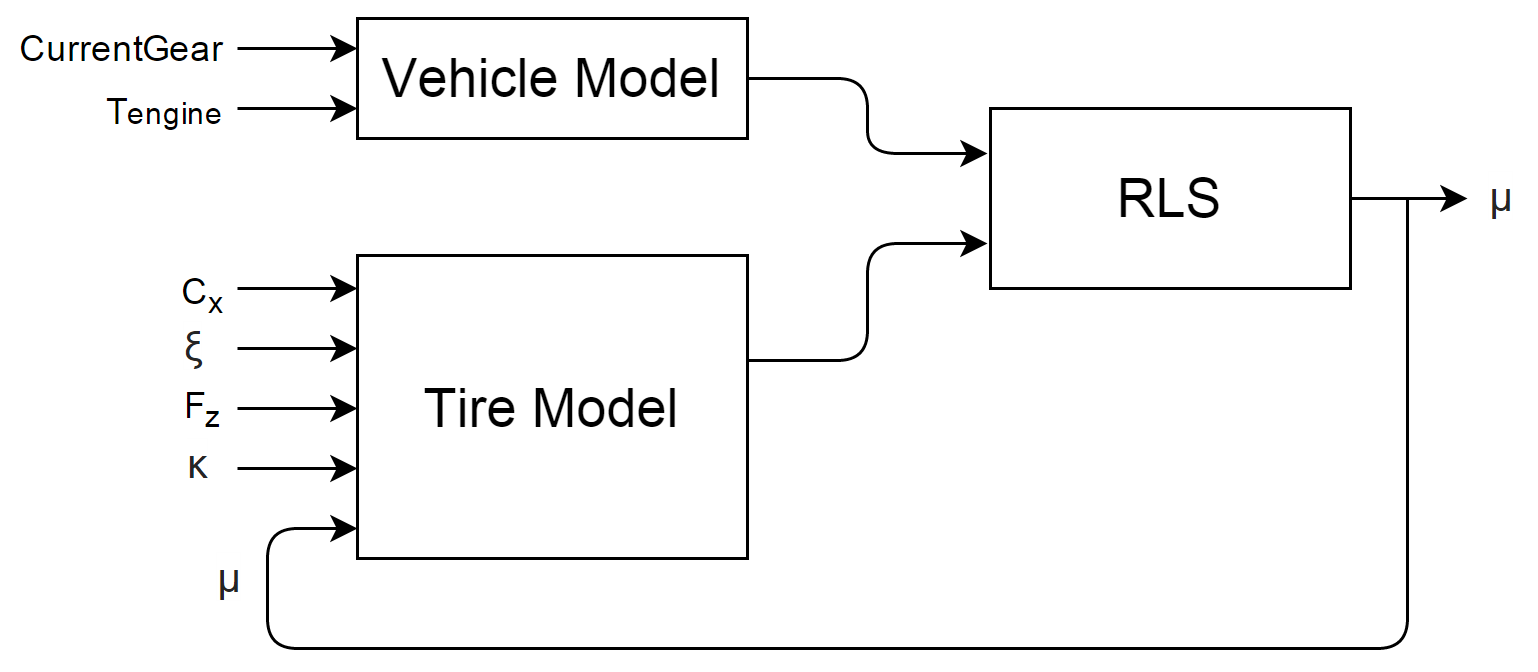
\includegraphics[width=1.0\textwidth]{Pictures/friction_estimator}
	\caption {Simple flow chart of the friction estimator.}
	\label{friction_estimator}
\end{figure}

One of the first parts of method includes calculations of the forces acting on the vehicle by using a vehicle model. This is for example done by using measured and calculated parameters such as wheel speed, yaw rate and acceleration but it can be done in other ways as well. Two different models that describes the vehicle forces will be presented in this work. 

Another part is to calculate the forces generated by the tires through a tire model. Such a model often depend on the tire stiffness, the tires slip ratio, the normal force acting on the tire and the road friction coefficient. Several tire models exists today and in this work four of them is considered. One of them is ruled out almost immediately, two of them is ruled after some more examination and the fourth is the one that is used. More on this later on.

Recursive least square fitting is a well known fitting method with fast convergence and good features such as forgetting factor. This method will be explained in detail as well.

\subsection{Practical restrictions and problems}
The idea presented above might sound like a very simple solution but there are several problems that have to be considered. The most important aspect that has to be taken into account is the fact that the friction estimation model has to work in a real car handled in actual driving situations. In a theoretical world, where a vehicle and a tire model is fed unbiased data, the friction coefficient can be obtained with good certainty and quite fast. Unfortunately, in the practical world, the data fed to the models are far from optimal. Things like measurement noise and approximative calculations corrupts the results. Several more complex driving situations are also hard to model correctly. This can for example be excessive wheel spin, aggressive cornering or speeds close to zero.

The true dynamics of both a vehicle and a tire is very complex and therefore also difficult to describe accurately with a model. At the same time, a model that is to be used has to be simple enough so that calculations are possible on an micro controller unit with limited computational power. Even though many simplified models are shown to be accurate enough to reflect reality in most driving situations, there are times when a simplified model inaccurately describes the detailed dynamics of a vehicle or a tire. 

There are also numerous models that uses parameters which are hard to measure or approximate well in reality. Some of these parameters includes the lateral velocity and slip angle. It is therefore desired to have a model that doesn't rely on these parameters. There are also car specific parameters, some which change between driving sequences, that can have a large impact on the modeled results. A few of these parameters includes the mass of the vehicle, wheel radii, lengths from center of gravity to the rear and front axle and the center of gravity height. The same goes for tires. When changing from winter tires to summer tires the tire stiffness will change a lot which will have a large impact on the results from the tire models. When using simulations, the exact value of these parameters can be known, but in a real environment they either have to be static, approximated or neglected in computations.

\subsection{FXD}
The problem stated in this work is to estimate the tire/road friction for a car using an FXD. This results in a number of conditions that have to be thought of and applied throughout the research. First of all, cars with an FXD installed are solely front wheel driven, meaning that there are no positive longitudinal forces acting on the rear wheels. The velocity of the rear wheels can therefore in most cases be used as a good approximation of the vehicles reference speed. Through the same reasoning, the longitudinal acceleration of the car can be derived from the derivative of the rear wheel velocities. There is also no steering done by the rear wheels.

Another aspect that has to be considered is that the FXD is an active limited slip differential, which means that the torque applied to the two driving shafts can differ in certain situations, unlike a car equipped with a standard open differential.

\subsection{Related work}
There have been quite extensive amount of research within this field of study and many different model proposals related to friction estimation during the last decades. The outcome of these researches usually show promising results, where the proposed solution works well during simulations and/or testing. Related work has provided a lot of information and help to this work, especially when it comes to getting a general understanding of the problem and its difficulties. But due to the fact that many results are based on theoretical simulations, a lot of information could be of little use or in some cases even be misleading.

\subsection{Conclusion}
All in all it is a great challenge to estimate the tire/road friction coefficient. \todo{Make sure this is true.} The approach, all of the problems mentioned and how they were taken care of will be explained in greater detail later on in the report.

\section{Signal processing}

Apart from the fact that a vehicle is hard to model properly, there is an uncertainty from the signals taken from the vehicles CAN bus. The true parameter values can be distorted from measuring and process noise as well as being delayed due to calculations and approximations. Different parameter signals can have varying distortions, and therefore include various challenges.

\subsection{Filters}

The signals that are taken from the vehicles CAN bus usually include quite a lot of noise and can cause severe succeeding errors during calculations and approximations. This measure and process noise mainly consist of sudden unwanted changes of the signal that generally has higher frequency than the true parameter value. To exclude these high frequencies, the signal is run trough a low pass filter which will dampen the amplitude of the higher frequencies. The amount of damping for certain frequencies depends on the filters cutoff frequency. 

In figure \ref{filter_and_no}, the filtered and unfiltered values can be seen for two signals, one of the wheel speeds and the engine torque. It can be seen that the noise of the signals are reduced after filtering, but to a cost of a delaying the signal. The sudden drop of the engine torque, at around $ 11 $ seconds, appears due to a gear change. This sudden drop of engine torque will be seen as a high frequency and is therefore incorrectly suppressed by the low pass filter.

\begin{figure}[h]
	\centering
	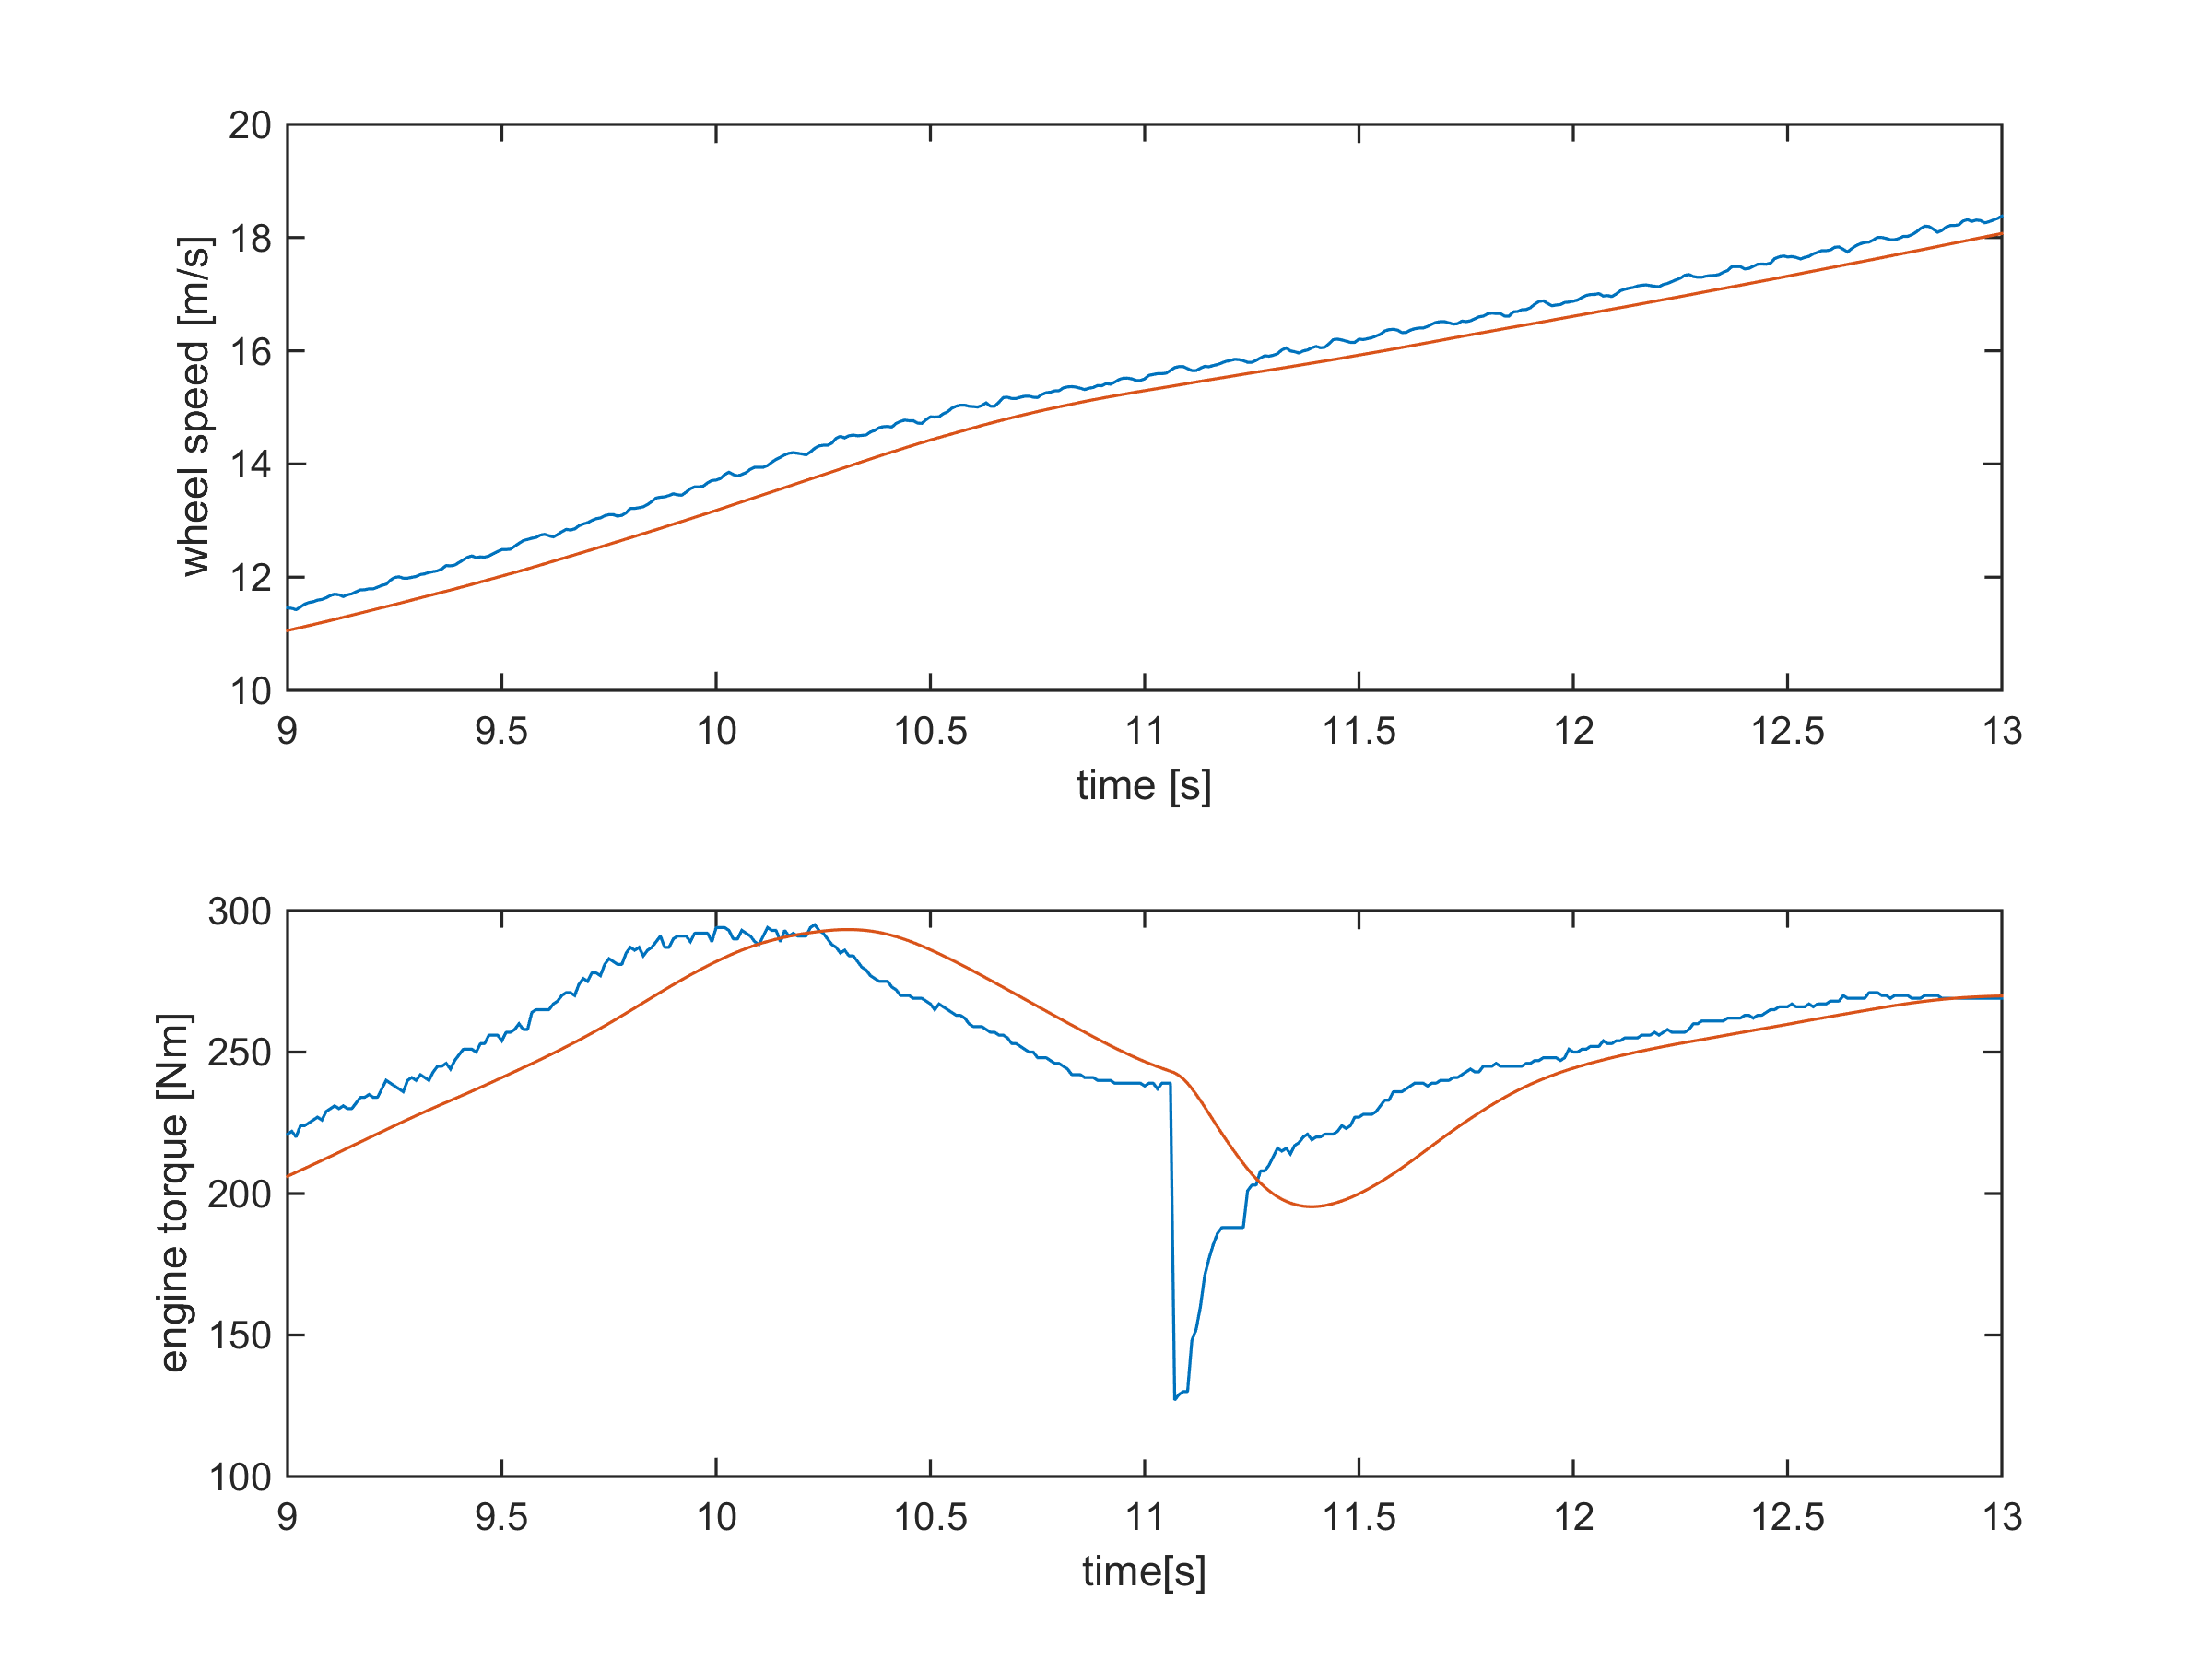
\includegraphics[width=1.0\textwidth]{Pictures/filter_and_no}
	\caption {Wheel speed and engine torque both unfiltered and filtered.}
	\label{filter_and_no}
\end{figure}

The amplitude and frequency of the noise will differ for various signals and could therefore  be filtered with different cutoff frequencies to get the most correct value. For example, the engine torque signal, seen in $ \ref{filter_and_no} $ subplot 2, could be filtered with a higher cutoff frequency than the wheel speed, seen in $ \ref{filter_and_no} $ subplot 1, to capture its faster changing characteristic better. However, an important aspect to consider during filtering, is the duration of the delay that will affect the signal. Signals that are run through filters with different cutoff frequencies, will also have differing delay durations. In the extent, this could lead to computations that should equal one another will differ greatly due to their different parameter dependencies. 

In figure $ \ref{different_filter_val} $, two different force models, that should be equal to each other, are dependent on different parameter values. In subplot one, a signal that affects the tire model is filtered with a cutoff frequency significantly lower than the cutoff frequency for the parameters affecting the vehicle model. In the extent, the force calculated from the tire model becomes delayed compared to the computed vehicle force. In subplot 2 however, the signals are filtered with the same cutoff frequency, hence resulting in a better match between the two models. The conclusion from this is that the low pass filters should not only be designed to get the best possible accuracy for that specific parameter, but the succeeding effects also need to be considered.

\begin{figure}[h]
	\centering
	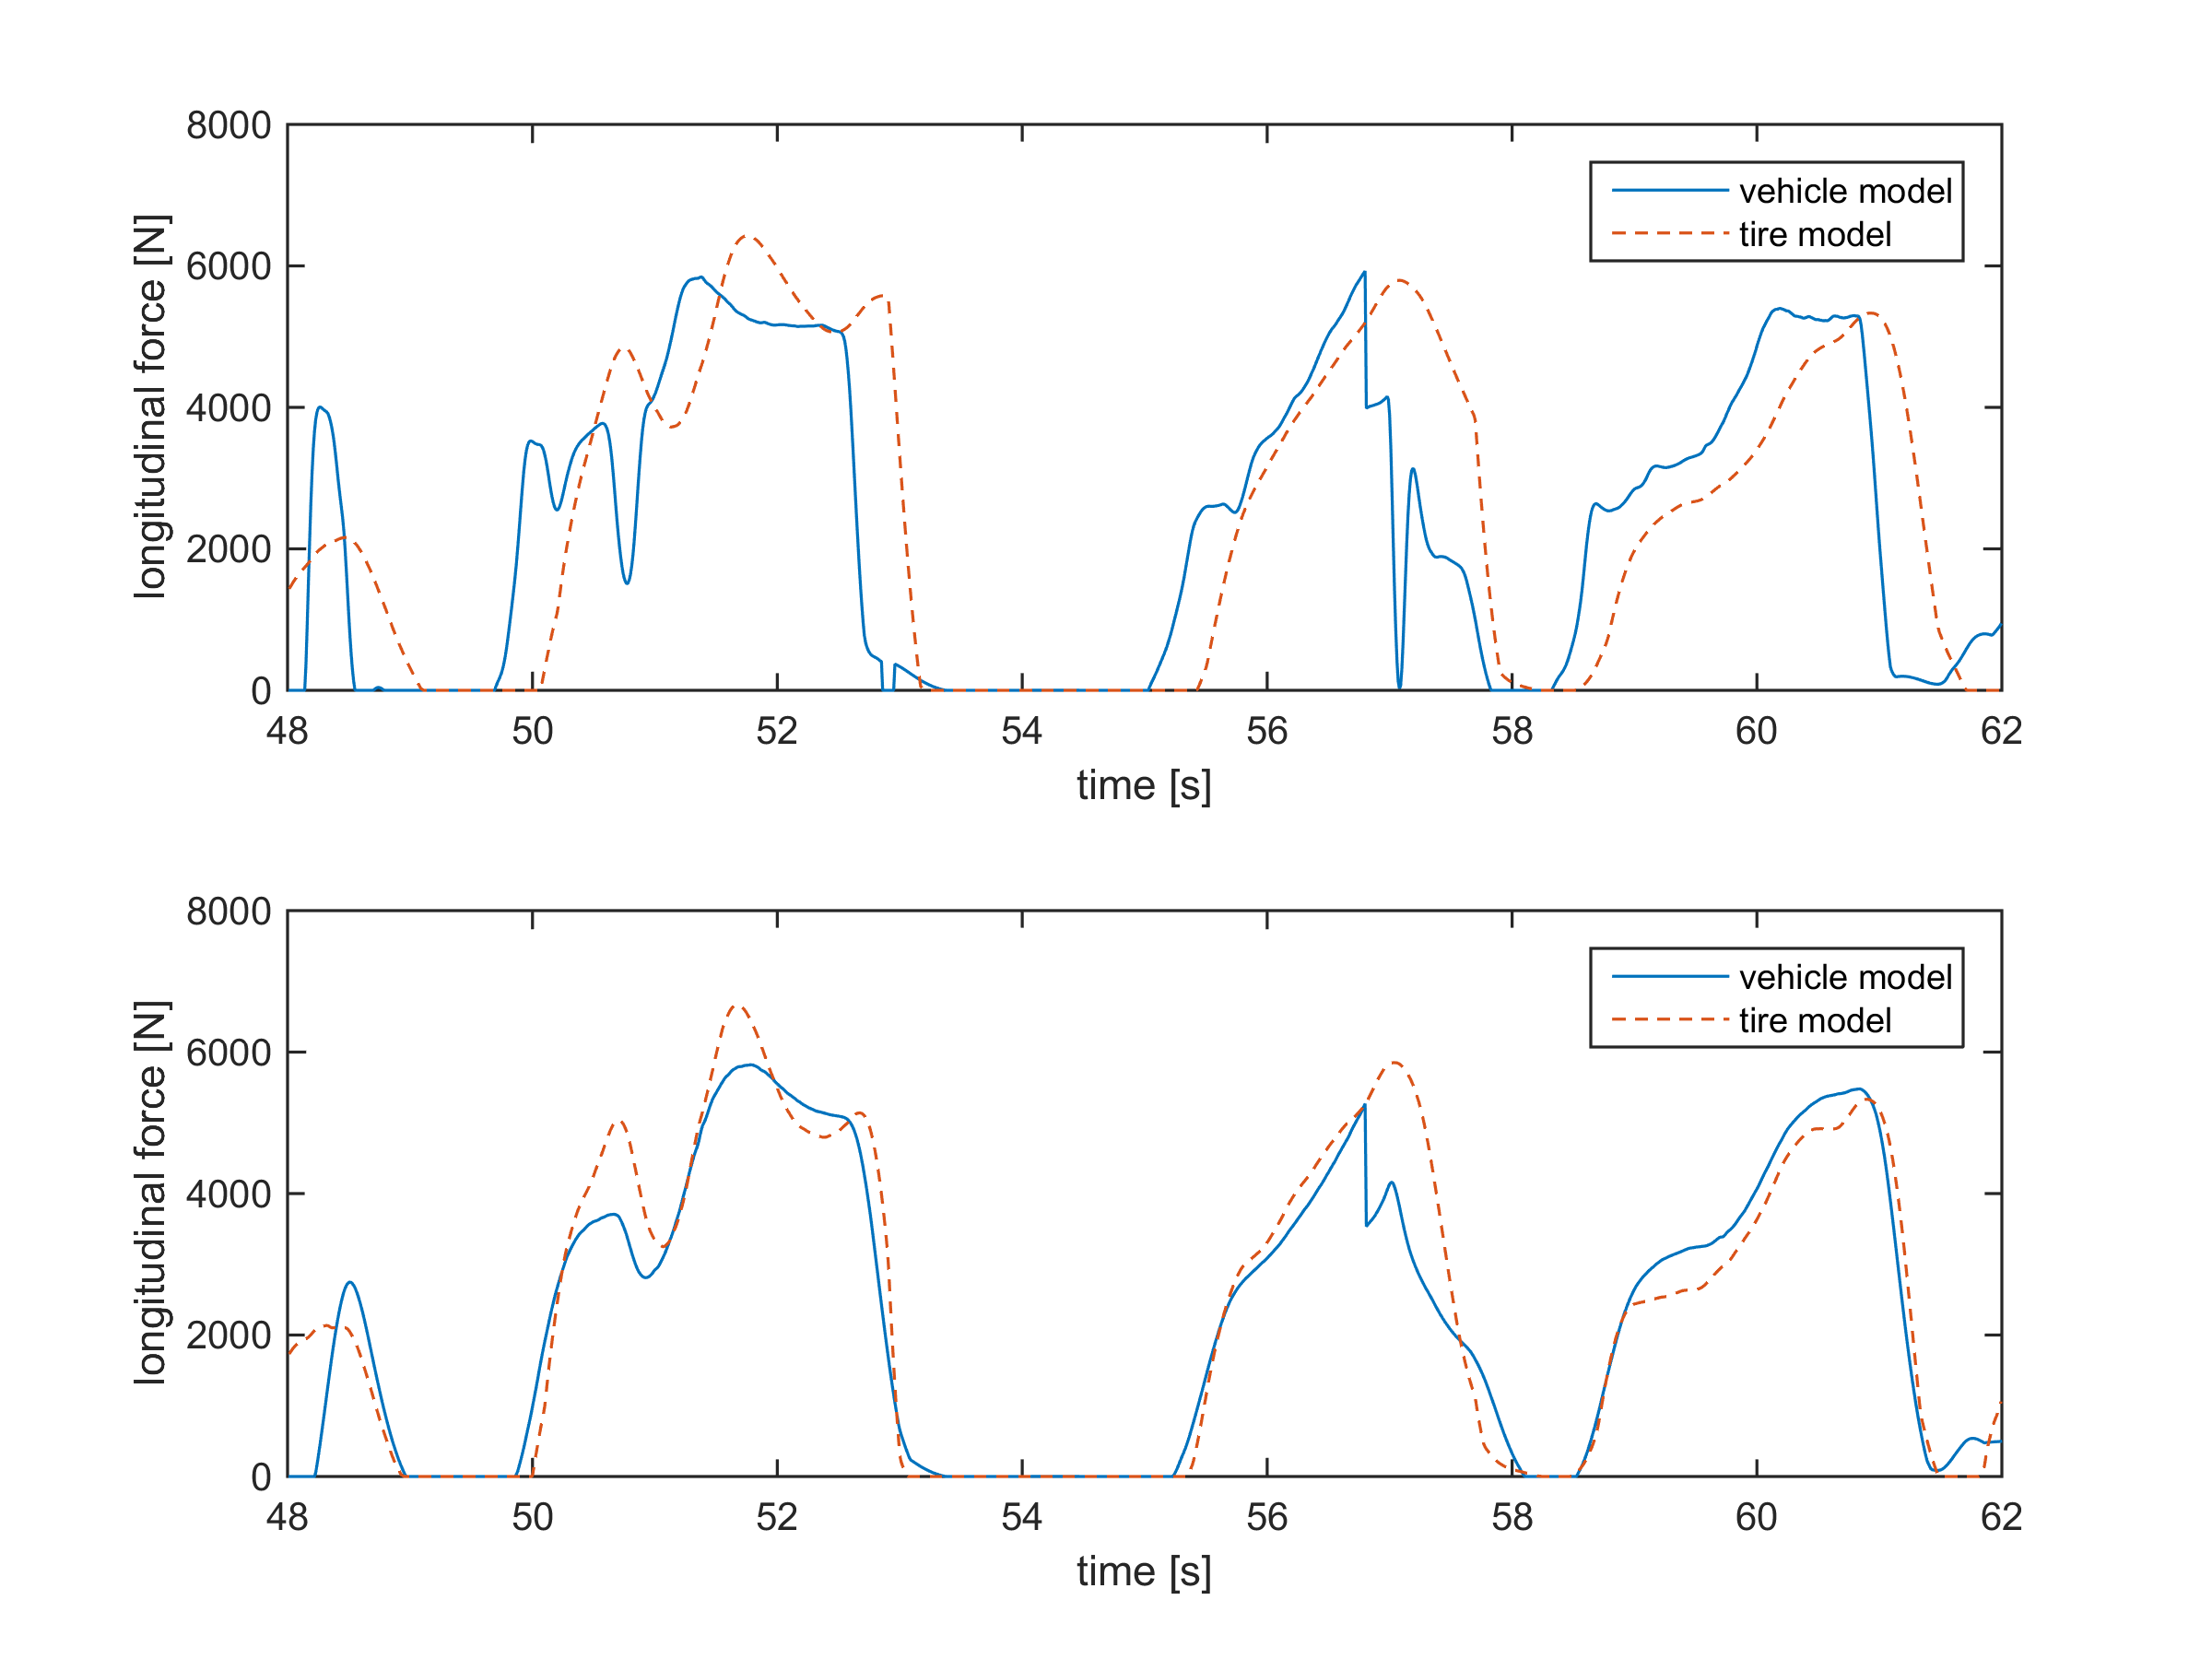
\includegraphics[width=1.0\textwidth]{Pictures/different_filter_val}
	\caption {Vehicle and tire model forces with different filter values for engine torque and wheel speeds.}
	\label{different_filter_val}
\end{figure}

\subsection{Static parameter impact} 
Even if a model can recreate a driving sequence correctly, there will always be an uncertainty due to vehicle specific parameters that are used. Some of these parameters include the position of the CoG, the radius of the wheels and the mass of the vehicle. The position of the CoG will affect the lengths from the CoG to the two axles, denoted $ l_{f} $ and $ l_{r} $ respectively, and also the CoG height from the ground. The position of the CoG will change depending on how the vehicle is loaded. The radius of the wheels can change slightly over time as the tire pressures changes, and can also be different from each tire. The radius of the wheel is used to calculate the velocity of the wheel and also to convert axle torque to force generated at the edge. The mass of the vehicle can change between different driving sequences, depending on how many persons that are seated within the car and also on additional weight. The vehicles mass and CoG height is used to calculate the weigh distribution and therefore also the amount of downward force generated at each tire. 

To get an understanding of how much these parameters affect the result, the force generated from two models with differing parameter values are seen in figure \ref{force_diff_re_mass}. In the first subplot, the longitudinal force is calculated from a vehicle model that approximates the torque applied to the two driving shafts and thereafter the force generated to the ground by using two different radii. A radius difference of $ 3 $ cm would be very large if considering a tire pressure drop, but could be possible when changing between wheels. In the second subplot, the longitudinal force calculated from a tire model is presented. The two different masses correspond to a vehicle with merely a driver respectively a vehicle with 5 persons. 

\begin{figure}[h]
	\centering
	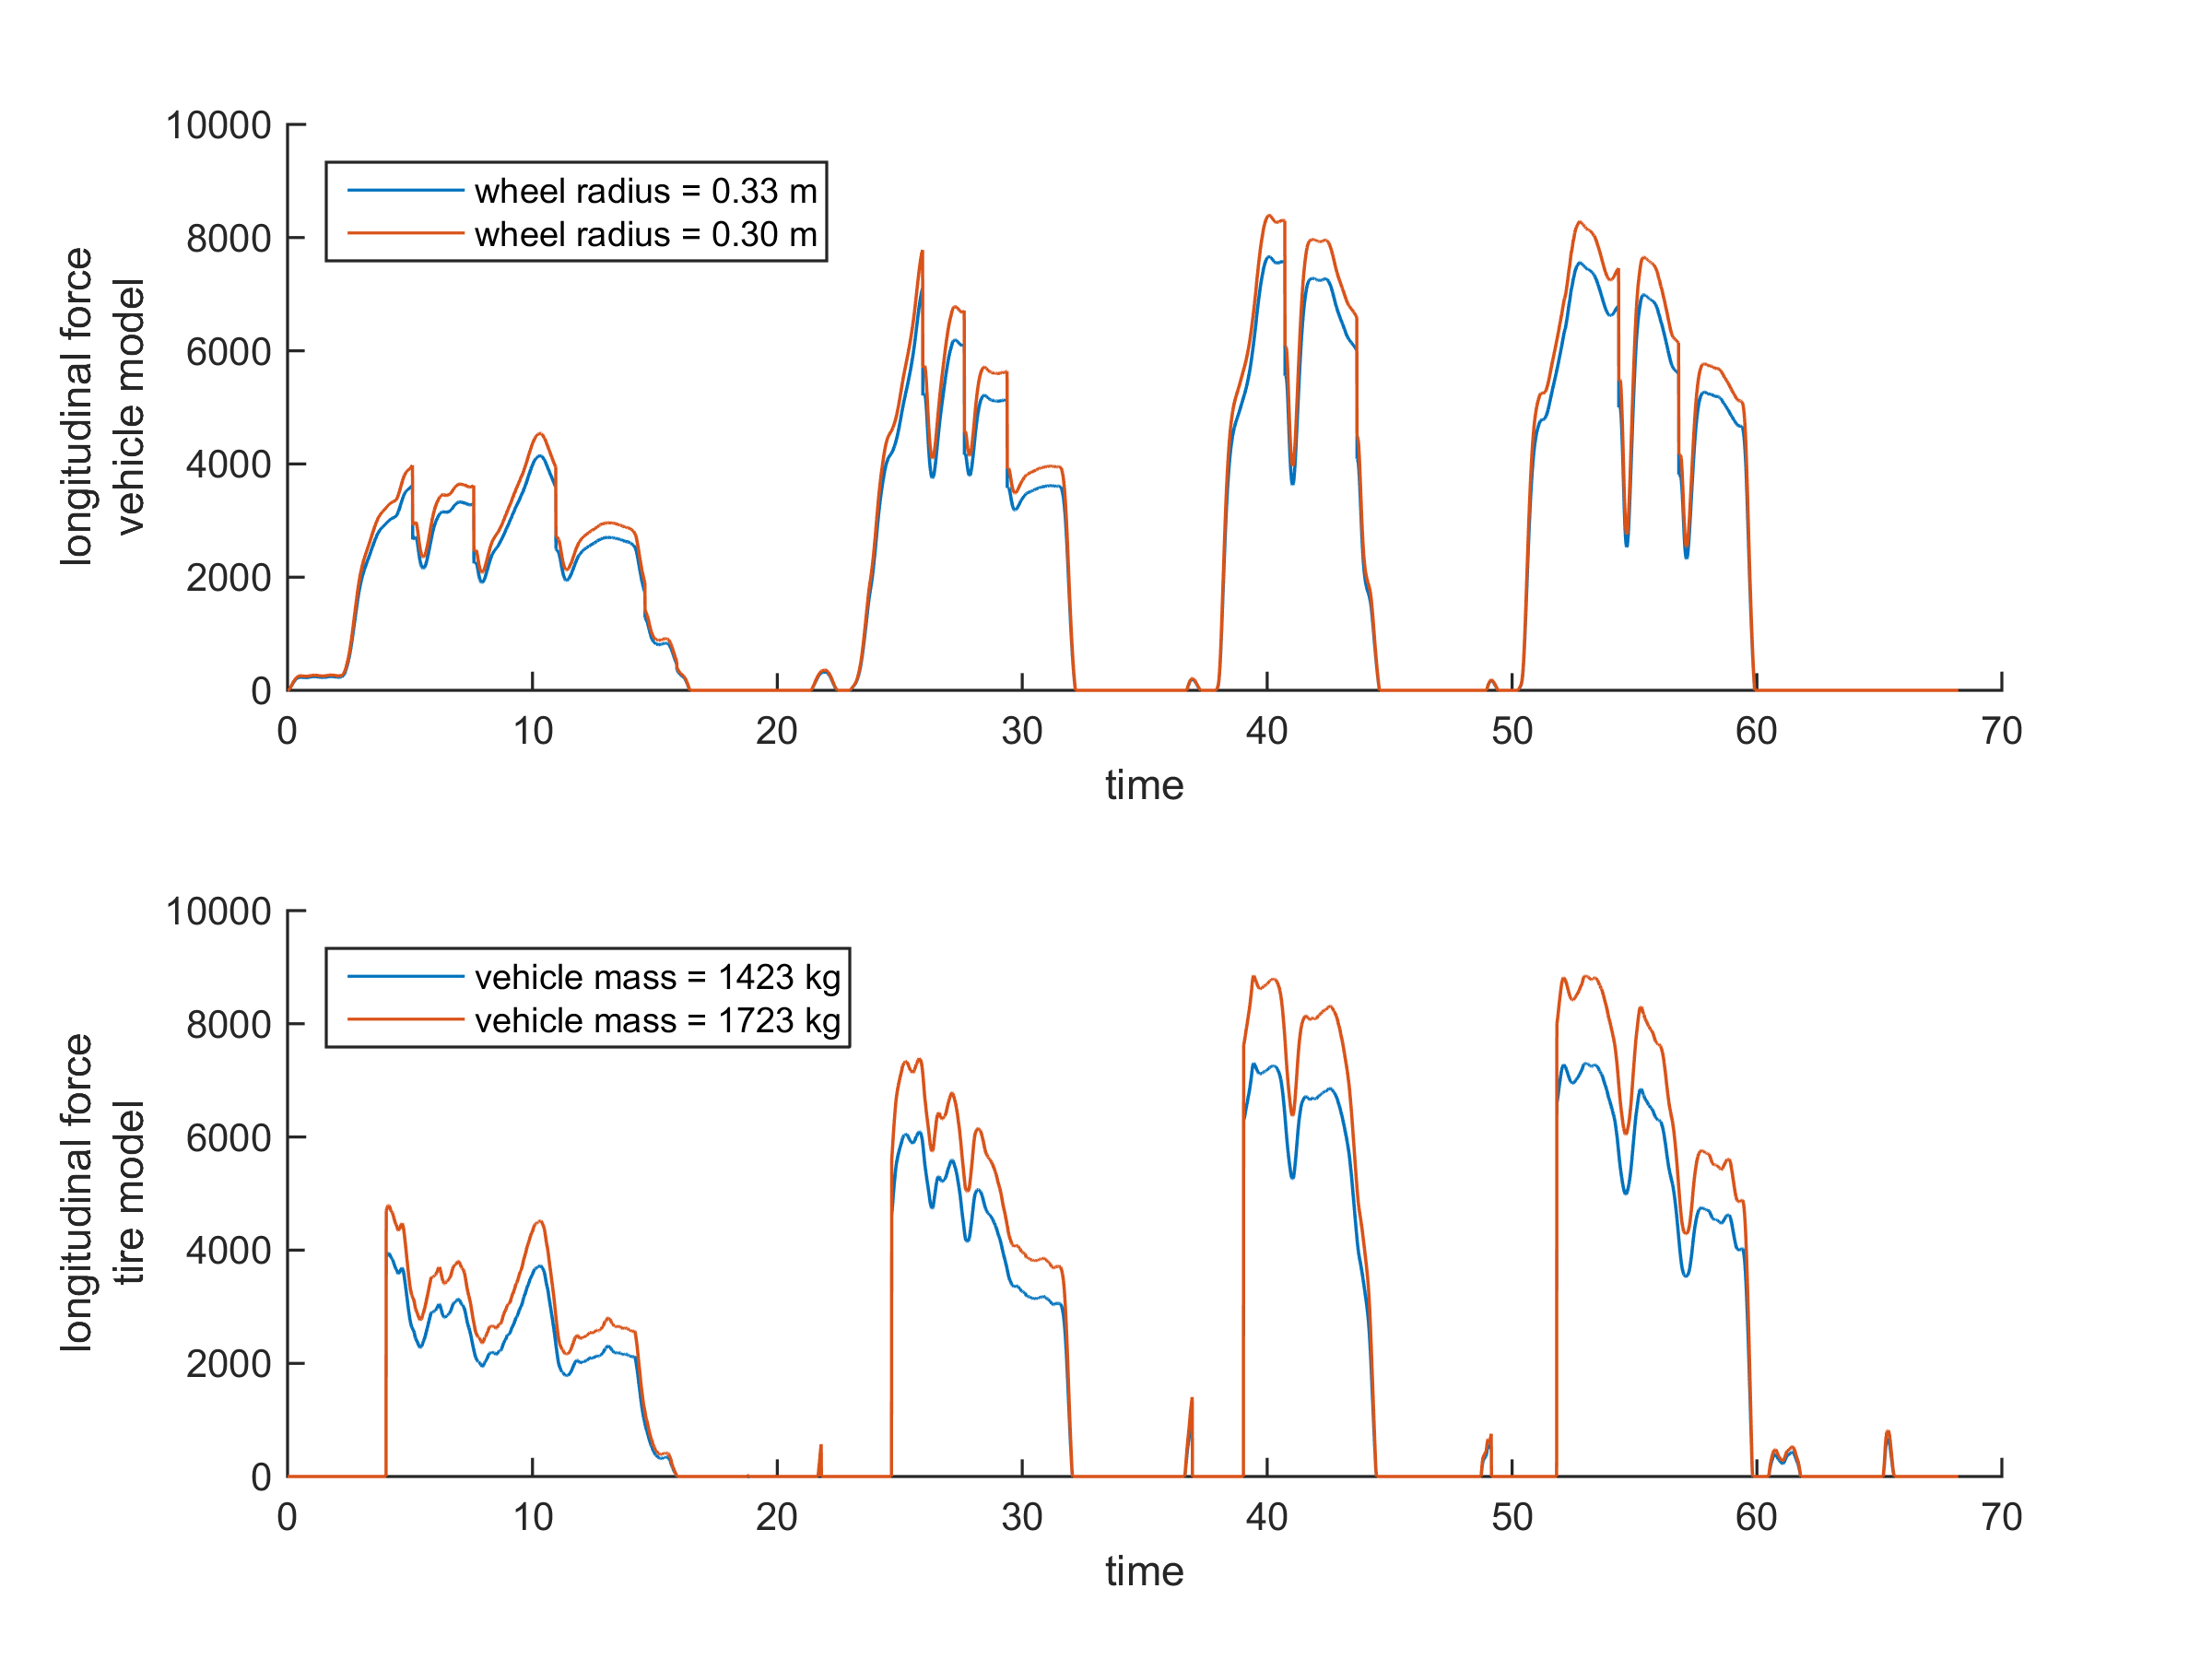
\includegraphics[width=1.0\textwidth]{Pictures/force_diff_re_mass}
	\caption {Forces for different wheel radii and masses.}
	\label{force_diff_re_mass}
\end{figure}

\section{Vehicle forces}
There are several forces acting on a vehicle. The largest forces are generated between the tires and the ground because the tires are the only parts of a car that have any physical contact with the surrounding world. While accelerating and braking longitudinal forces will arise and while cornering lateral forces will arise. The tires are responsible for all the forces that actually control the vehicle which makes them very important for good handling but also makes them hard to model. Beside these major forces there are also forces such as wind drag and rolling resistance acting on the vehicle.

The trick is to calculate all the forces into one total force that can be compared to the total force generated by the tires.
\subsection{Vehicle force calculated from longitudinal acceleration}
The simplest way of representing the force acting on the vehicle while accelerating is to use the acceleration and the mass of the car and apply Newtons second law of motion:
\begin{equation}
	F = m \cdot a
\end{equation}
\subsubsection{Estimating the longitudinal acceleration}
\label{longaccest}
For this method to be accurate an accurate estimation of the longitudinal acceleration is needed. Some cars have accelerometers installed for longitudinal measurements which makes it straight forward to calculate the force. If one of those aren't available the acceleration has to be calculated instead. This can be done by derivation of the vehicles speed. The speed of the vehicle can be obtained by measuring the speeds of the undriven wheels. For a FWD car this would be the rear wheels. To make the calculation more accurate the average speed of the two rear wheels is calculated before the derivation is done.
\begin{equation}
a_{x} = \frac{d}{dt}(\frac{w_{rl}+w_{rr}}{2})
\end{equation}

\subsubsection{Estimating the losses}
Two different losses are compensated for. Losses from drag and losses from rolling resistance.

The drag force is calculated as:

\begin{equation}
F_{D}=\frac{1}{2}\rho v^2 C_{d}A
\end{equation}
where:
\begin{itemize}
	\item $ \rho $ is the density of air.
	\item $ v $ is the speed.
	\item $ C_{d} $ is the drag coefficient.
	\item $ A $ is the cross sectional area.
\end{itemize}
The rolling resistance is calculated as in Equation \ref{eq:rollingres}.

\subsubsection{Estimating the total vehicle force}
The total amount of force acting on the vehicle thus becomes: \todo{this formula might be altered}
\begin{equation}
\label{eq:newton}
F_{vehicle} = m \cdot a + F_{drag} + F_{rolling resistance}
\end{equation}

\subsubsection{Complications}
The main issue with this method is that it's based on longitudinal acceleration and longitudinal losses only, hence it can only be used to estimate the vehicle forces when accelerating in a straight line. Although this is a big restriction it might be enough since acceleration in a straight line happens pretty often while driving.

A major hardship is to obtain a proper value for the longitudinal acceleration. If the vehicle doesn't have an accelerometer the acceleration calculated from the wheel speeds needs to be used. This immediately causes problems when the vehicle is accelerating on a gradient road. During an uphill acceleration, the actual force to accelerate the vehicle will be higher than the force calculated from Newtons second law. Driving downhill, the force will be lower. This is because the earths gravity isn't considered in the formula. When climbing a hill the vehicle force needs to include the force of the earths gravitational pull as well. The same goes for then driving downhill, but now the force will instead help accelerating the vehicle. The force of the gravitational pull can be calculated if the angle of the vehicle relative the earths horizontal plane is known but this angle is hard to measure or estimate. \todo{is it really?}

Measuring it with an accelerometer ......\todo{does it work good or bad in hills?}

The second parameter of Newtons second law is the mass which also is hard to estimate. The mass of the vehicle can vary several hundreds of kilos depending on passengers and load in the trunk. A Golf GTi has a curb weight of about 1350 kg. Hence, the varying weight of several hundreds of kilos will have a great impact on the force calculations. To counter this problem some kind of load detection needs to be available to set a new mass every time the car is driven. This isn't something that is very common on cars today and thus a static mass of the vehicle needs to be set resulting in errors in the force calculations way too often.

Suppose that the force calculation from Newtons second law is correct. Still there are losses to be accounted for. They need to be calculated properly to be able to compare the vehicle force to the tire force. Looking at the formula above \ref{eq:newton}, two different losses are compensated for. The rolling resistance is straight forward if the rolling resistance coefficient is known. The drag is a bit more complicated but should prove to be fairly accurate as well if the parameters is known. All in all, the results of these calculations won't be perfect and there are several more losses that can't be calculated in any good way. \todo{are there really?}


\subsection{Vehicle force calculated from engine torque}
Another way of calculating the longitudinal force of a vehicle is to derive the actual torque that is applied to the shafts connected to the driven wheels. The advantage of using the engine torque, instead of the acceleration of the vehicle, is its independence of the roads gradient and losses such as wind drag and steering losses. The torque that is applied to the shafts will be directly proportional to the actual force generated by the wheels, regardless of how the gravitational pull and other losses are acting on the vehicle. 

The formula for calculating the total torque on the drive shafts is simple:
\begin{equation}
\label{eq:tshaft}
T_{driveshafts} = T_{engineshaft}\cdot GearRatio
\end{equation}
where the gear ratio is the speed ratio between the engine shaft and the differential housing:
\begin{equation}
\label{eq:GR}
Gear Ratio = \frac{RPM_{engine}}{RPM_{diffhouse}}
\end{equation}
and finally the speed of the differential housing is the average speed of the left and right drive shafts:
\begin{equation}
\label{eq:diffhouse}
RPM_{diffhouse} = \frac{RPM_{leftdriveshaft}+RPM_{rightdriveshaft}}{2}
\end{equation}
The engine torque, engine speed and the drive shaft speeds (wheel speeds) are all parameters commonly found on the CAN bus of a newer car. Important to notice is that these calculations do not consider any losses from the engine to the drive shaft. By combining equations $ \ref{eq:tshaft} $ and $ \ref{eq:GR} $, it is seen that the power generated by the engine and the power outputted to the drive shaft are equal.
\begin{equation}
P = T_{driveshaft}\cdot RPM_{driveshaft} = T_{engineshaft}\cdot RPM_{engineshaft}
\end{equation}

The torque will be split evenly between the two drive shafts, assuming an open differential, i.e. when the FXD is inactive. If the FXD is active the available torque on the drive shafts has to the redistributed according to the amount of torque being transfered through the FXD. This is important to consider if force calculations for a single wheel are to be done. 

When the torque on each drive shaft is calculated the force acting on each tire is calculated by dividing that torque by the wheel radius:
\begin{equation}
\label{eq:tireforce}
F_{tire} = \frac{T_{shaft}}{R_{e}}
\end{equation}
These forces can then be compared to the forces generated by the tire models for each tire.

\subsubsection{Gear ratio}
Calculating the gear ratio with Equations \ref{eq:GR} \& \ref{eq:diffhouse} gives varying results. Both the engine speed and wheel speed signals are noisy. In the gear change moment it will take some time for them to stabilize again resulting in long times of faulty force calculations. 

On newer cars it's not very uncommon to find what gear is active at the moment as a signal on the CAN bus. By knowing this the gear ratio can be set without any calculations since the gear ratio for each gear is known. For the Golf GTi the gear ratios can be seen in Table \ref{tab:gr}. A graph of the calculated and predefined gear ratio can be seen in Figure \ref{gear_ratio}. It can be seen that the calculated signal is much slower than the predefined one. It's also oscillating quite much which is bad because the gear ratio really is a static value purely depending on what gear is active. 


\begin{table}[position specifier]
	\centering
	\begin{tabular}{| l | l |}
		\hline
		Gear & Gear ratio \\ \hline
		1 & 13.9284 \\ \hline
		2 & 8.5383 \\ \hline
		3 & 5.4378 \\ \hline
		4 & 3.7206 \\ \hline
		5 & 2.7666 \\ \hline
		6 & 2.1942 \\ \hline
	\end{tabular}
	\caption{Gear ratios for the Volkswagen Golf GTi Mk7}
	\label{tab:gr}
\end{table}

\begin{figure}[h]
	\centering
	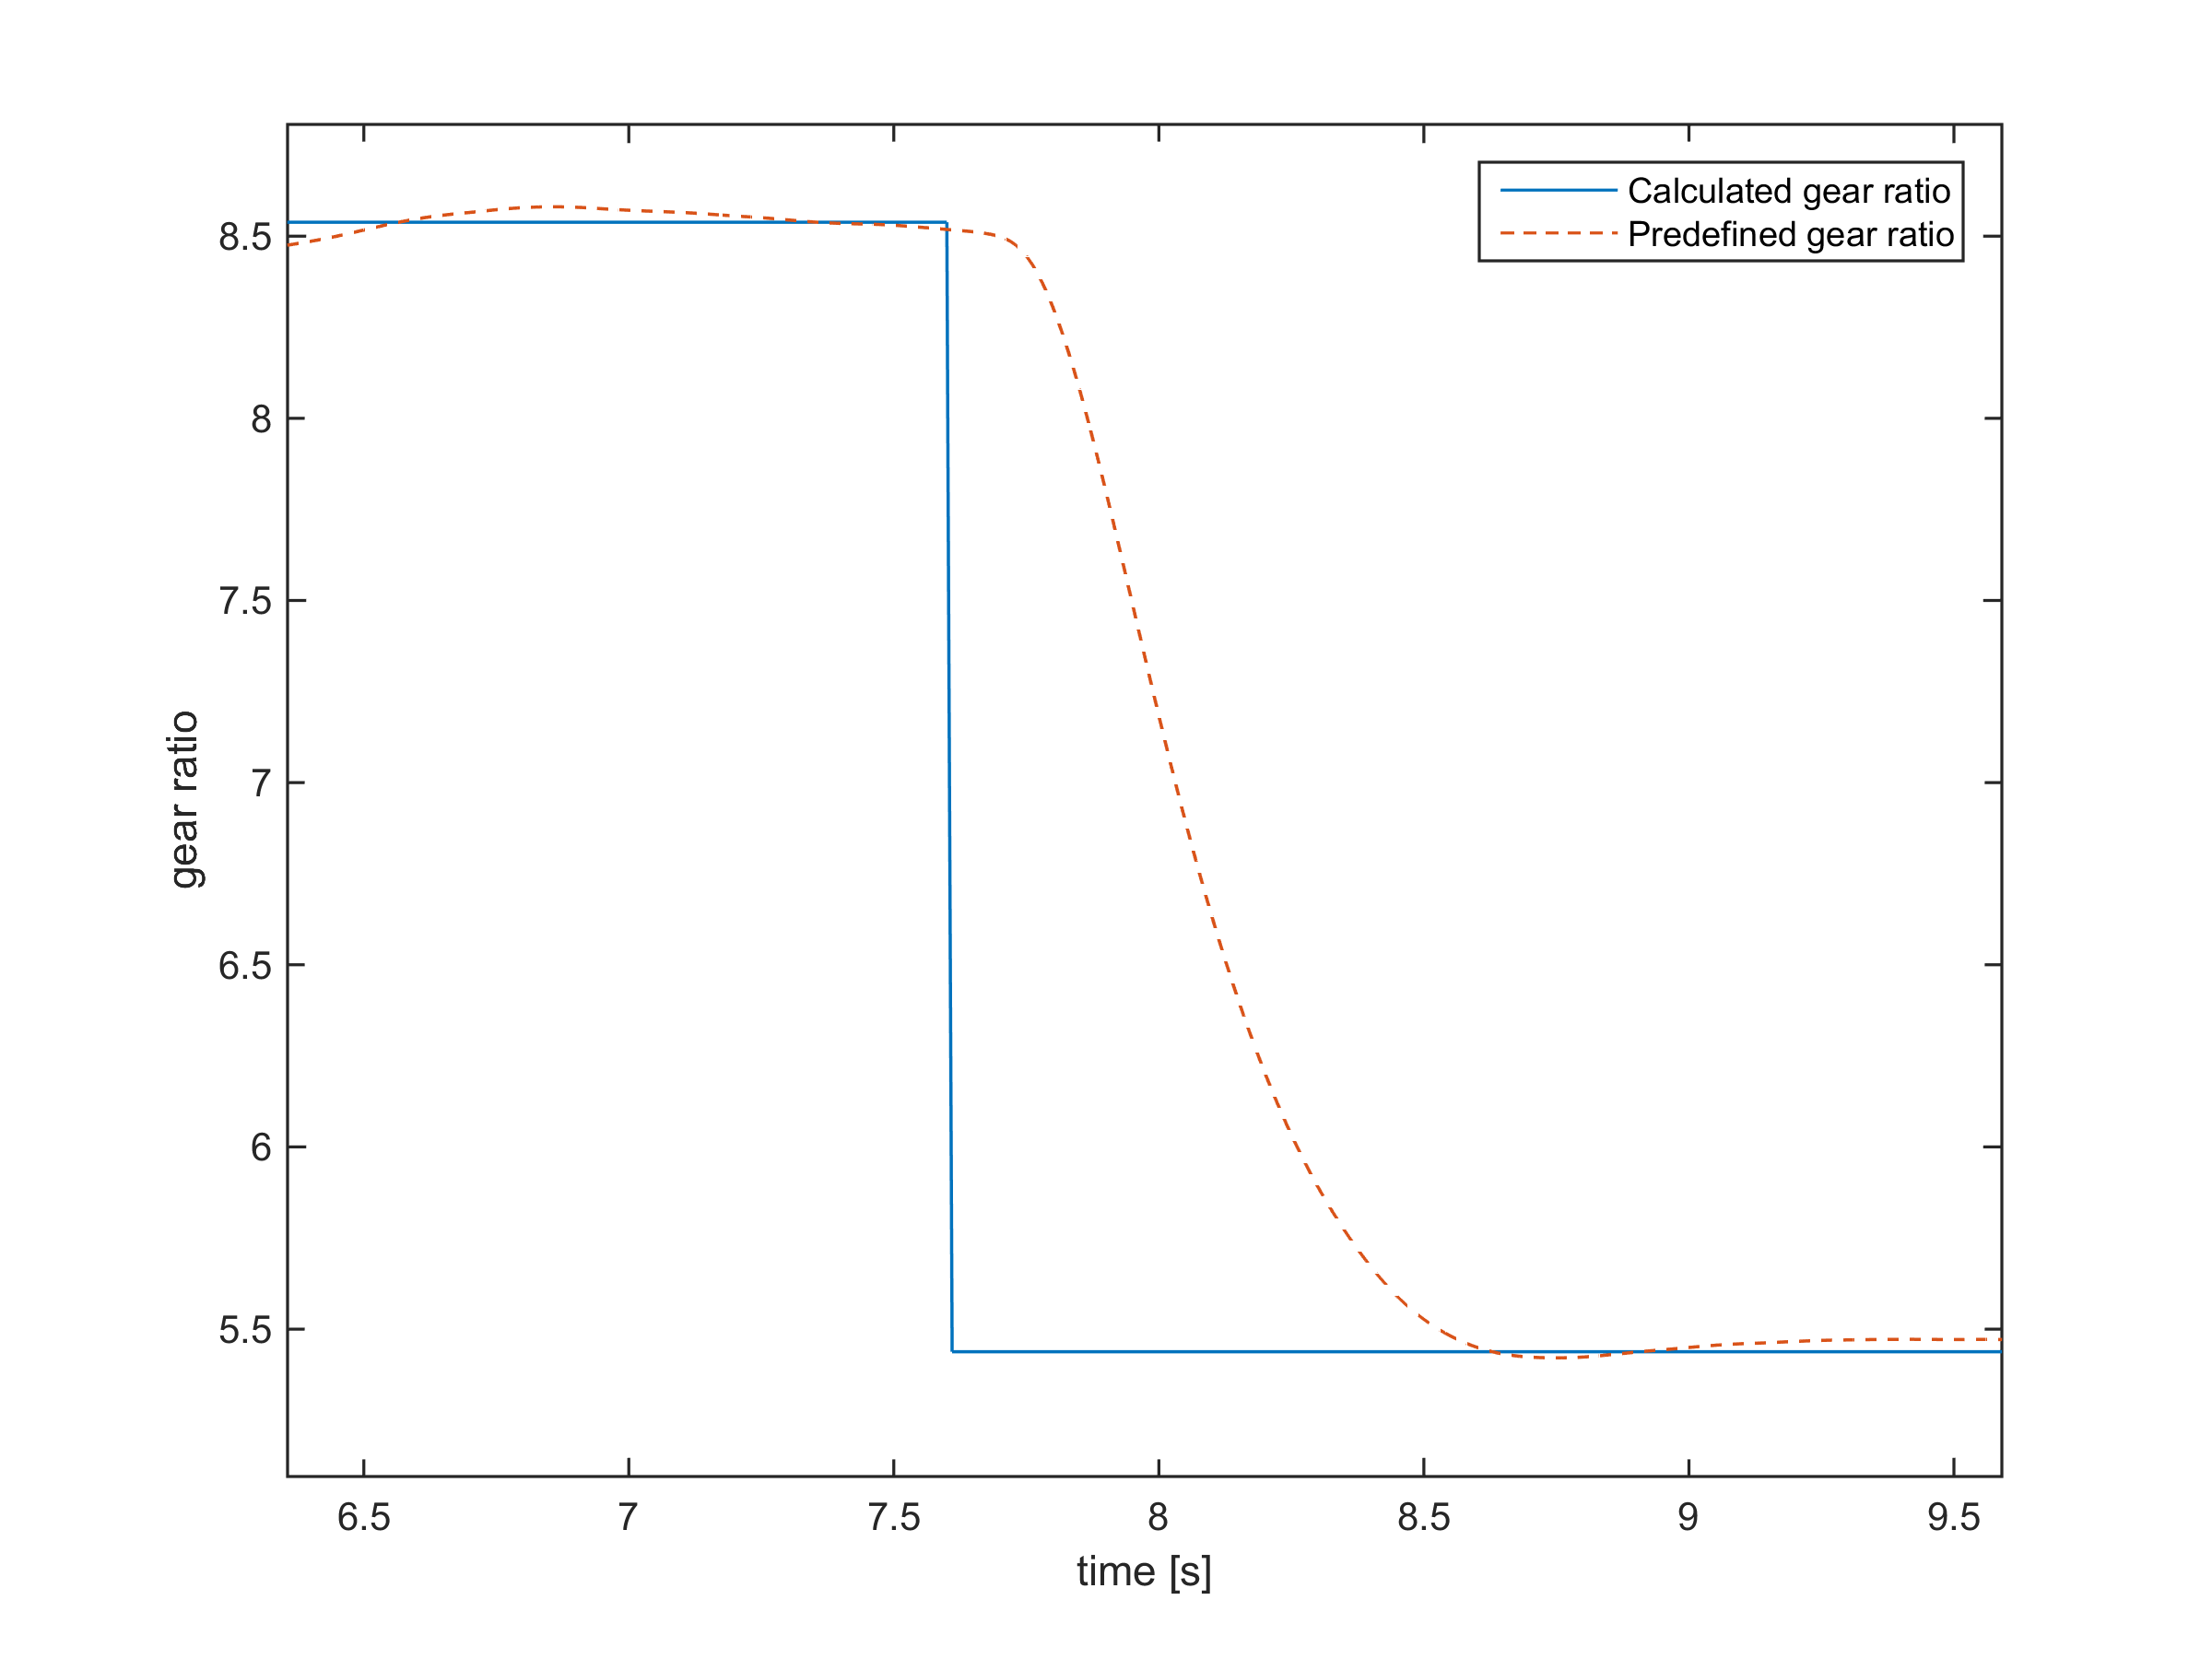
\includegraphics[width=0.8\textwidth]{Pictures/gear_ratio}
	\caption{Calculated and predefined gear ratio in a gear change from 2nd to 3rd gear.}
	\label{gear_ratio}
\end{figure}

\cite{mason}

\subsubsection{Transfer losses}
There are several factors that affect how much of the engine torque that actually becomes available on the drive shafts. There are several losses in a drive line. Friction and rotating masses within the drive line are the main contributors. Some torque are also lost accelerating the mass of the wheel itself.
\begin{equation}
T_{driveshaft} = T_{driveshaftwithoutlosses}\cdot\eta_{friction}\cdot\eta_{rotating mass} - T_{wheelacceleration}
\end{equation}
$ \eta_{friction} $ is just a scalar factor. The frictional losses are very dependent on the design of the drive line. This means that the losses will differ between vehicles and that this factor needs to be calculated for each specific car model. Since this factor is easy to change it will also include other losses in the drive line such as acceleration of the drive shafts. \todo{can we say this?}

$ \eta_{rotating mass} $ is modeled as:
\begin{equation}
\eta_{rotating mass} = \frac{1}{1 + factor(0.0025?)\cdot gearratio^2}
\end{equation}\\
\todo{choose factor}
The efficiency gets worse as the gear ratio gets higher since there will be more rotating mass in low gears. \todo{is this true?} Just as the frictional losses this loss is also dependent on the design of the drive line. Thus the factor multiplied with the gear ratio needs to be decided for each specific car model.

To calculate $ T_{wheelacceleration} $ requires some more steps. Each wheel connected to a driven shaft has its own moment of inertia which will be accelerated if enough torque is applied. The amount of torque needed to accelerate the wheel depends on its moment of inertia and the angular acceleration:
\begin{equation}
	T = a \cdot I
\end{equation}
The moment of inertia is the wheels radii squared and integrated over the mass. 
\begin{equation}
	I = \int r^2 \cdot dm
\end{equation}
Assuming that a wheel has the shape of a solid cylinder with equal amount of density throughout, the moment of inertia for a wheel can instead be described as:
\begin{equation}
	I = \dfrac{r^2 \cdot m}{2} 
\end{equation}
In the same manner, this applies for the actual drive shafts as well but as was said earlier this loss is included in the scalar factor describing the frictional losses. \todo{again, can we say this?}

The angular acceleration is calculated in the same manner as in Section \ref{longaccest} but now for the front left and right wheel separately.


\subsubsection{Complications}
\todo{this part needs more work}
The main issue with this method is the overall uncertainty of it. For example, the engine torque obtained from the CAN bus isn't measured with a torque sensor on the crankshaft but rather is a calculated value from the engine control unit. The engine control unit calculates the torque with the help several engine parameters and even if it's close most of the times there are moments when it isn't quite right. When doing a sudden acceleration that's aggressive enough to make the vehicle shift down some gears, a so called kickdown, the torque reading will be faulty. 

This method won't work during shifting because the link between the engine shaft and the drive shafts will be lost or affected while the clutch and transmission are working to shift gear. To avoid this trouble the vehicle force estimation simply needs to paused as soon as the start of a gear shift is detected.

\subsubsection{Verification}
Since the reliability of the method is uncertain is needs to be verified in some way. This was done with test data from a driving session where the vehicle was equipped with torque sensors mounted on the drive shafts. By comparing the results from the calculated torque values to the measured values the functionality of the method can be verified. Further on some basic tuning of the efficiency coefficients can be made. In Figure \ref{torque_ver} the verification can be seen.

\begin{figure}[h]
	\centering
	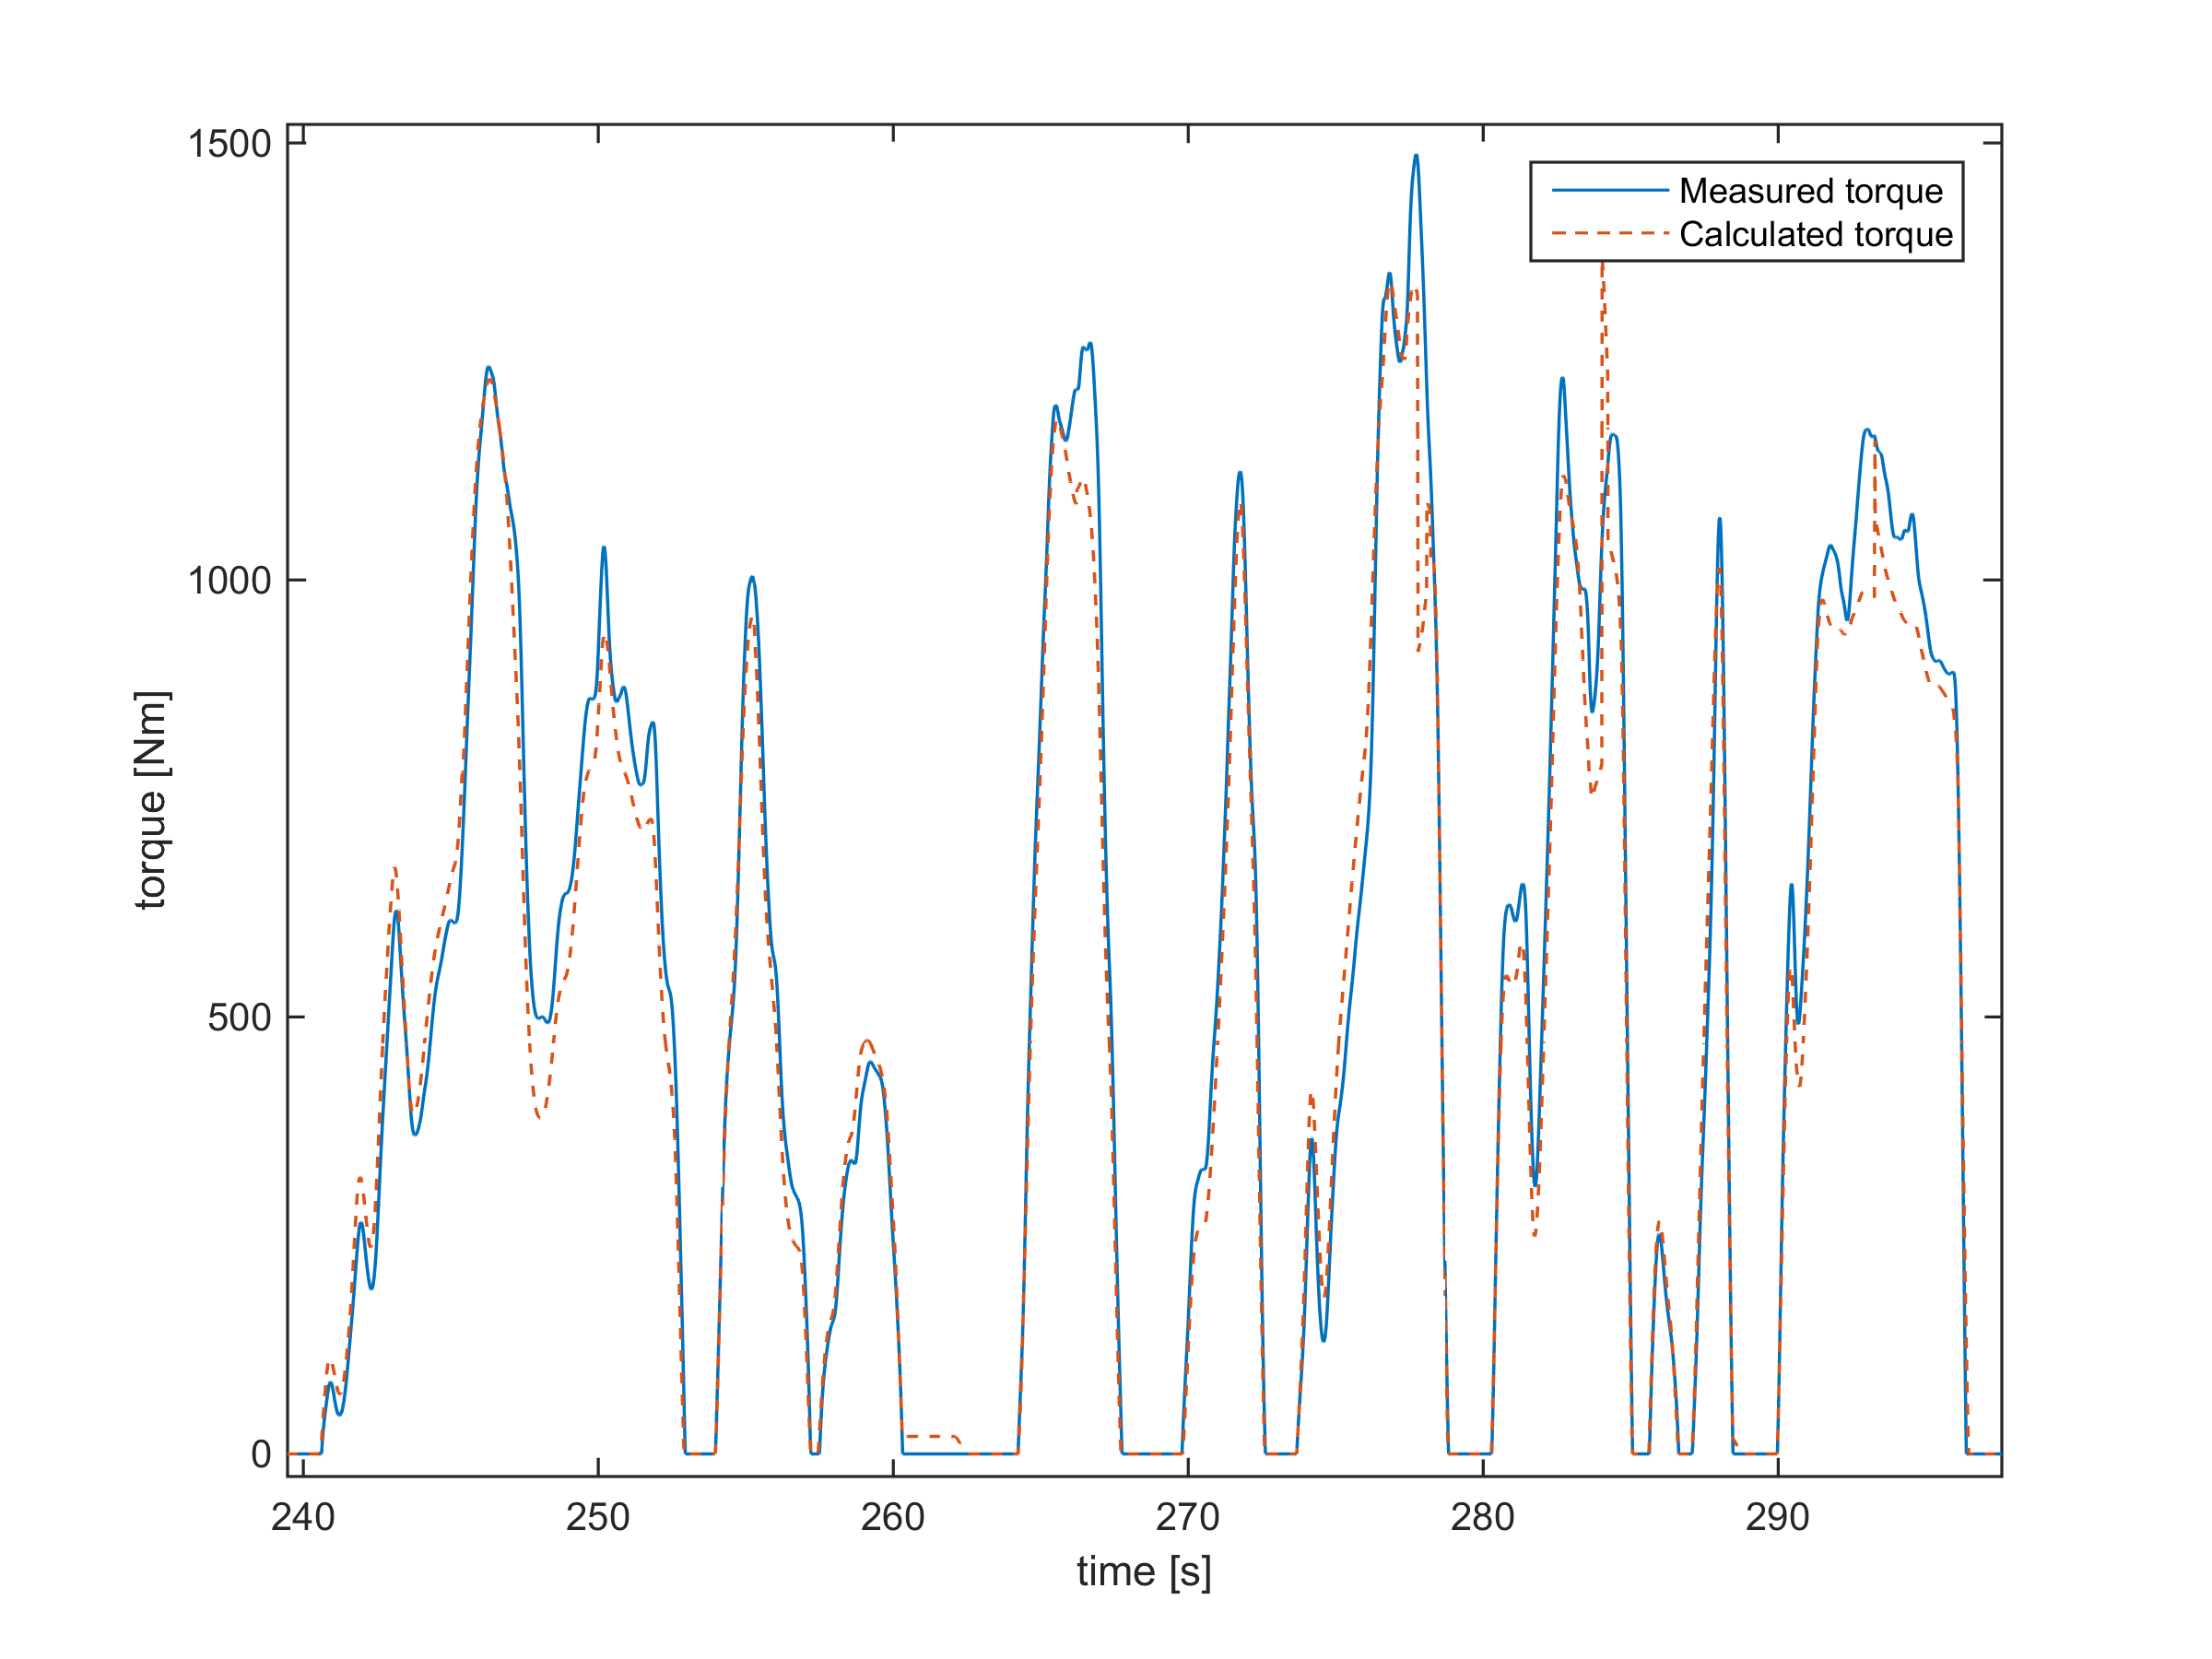
\includegraphics[width=1\textwidth]{Pictures/torque_ver}
	\caption{Measured and calculated torque on the left drive shaft from a vehicle equipped with torque sensors on the drive shafts.}
	\label{torque_ver}
\end{figure}

\subsection{Choosing vehicle model}
Two different models for estimating the vehicle force have been presented. One is based on calculating the force using Newtons second law. This model can be divided into two sub models since the vehicle acceleration can be calculated by derivation of the undriven wheel speed or measured with an accelerometer. The other model uses the engine torque to calculate the vehicle force. Thus, the vehicle force can be acquired in three different ways and it's of course desired to use the most accurate model. When driving in a straight line on a flat road these three models will result in almost the same force, as can be seen in Figure \ref{vehicle_model_comp_olikaacc}. The engine torque model will drop below the other models while shifting gear since the engine is disconnected from the wheels while doing so. This is something that has to be considered, more on this in Section \ref{sec:gearchange}. 

\begin{figure}[h]
	\centering
	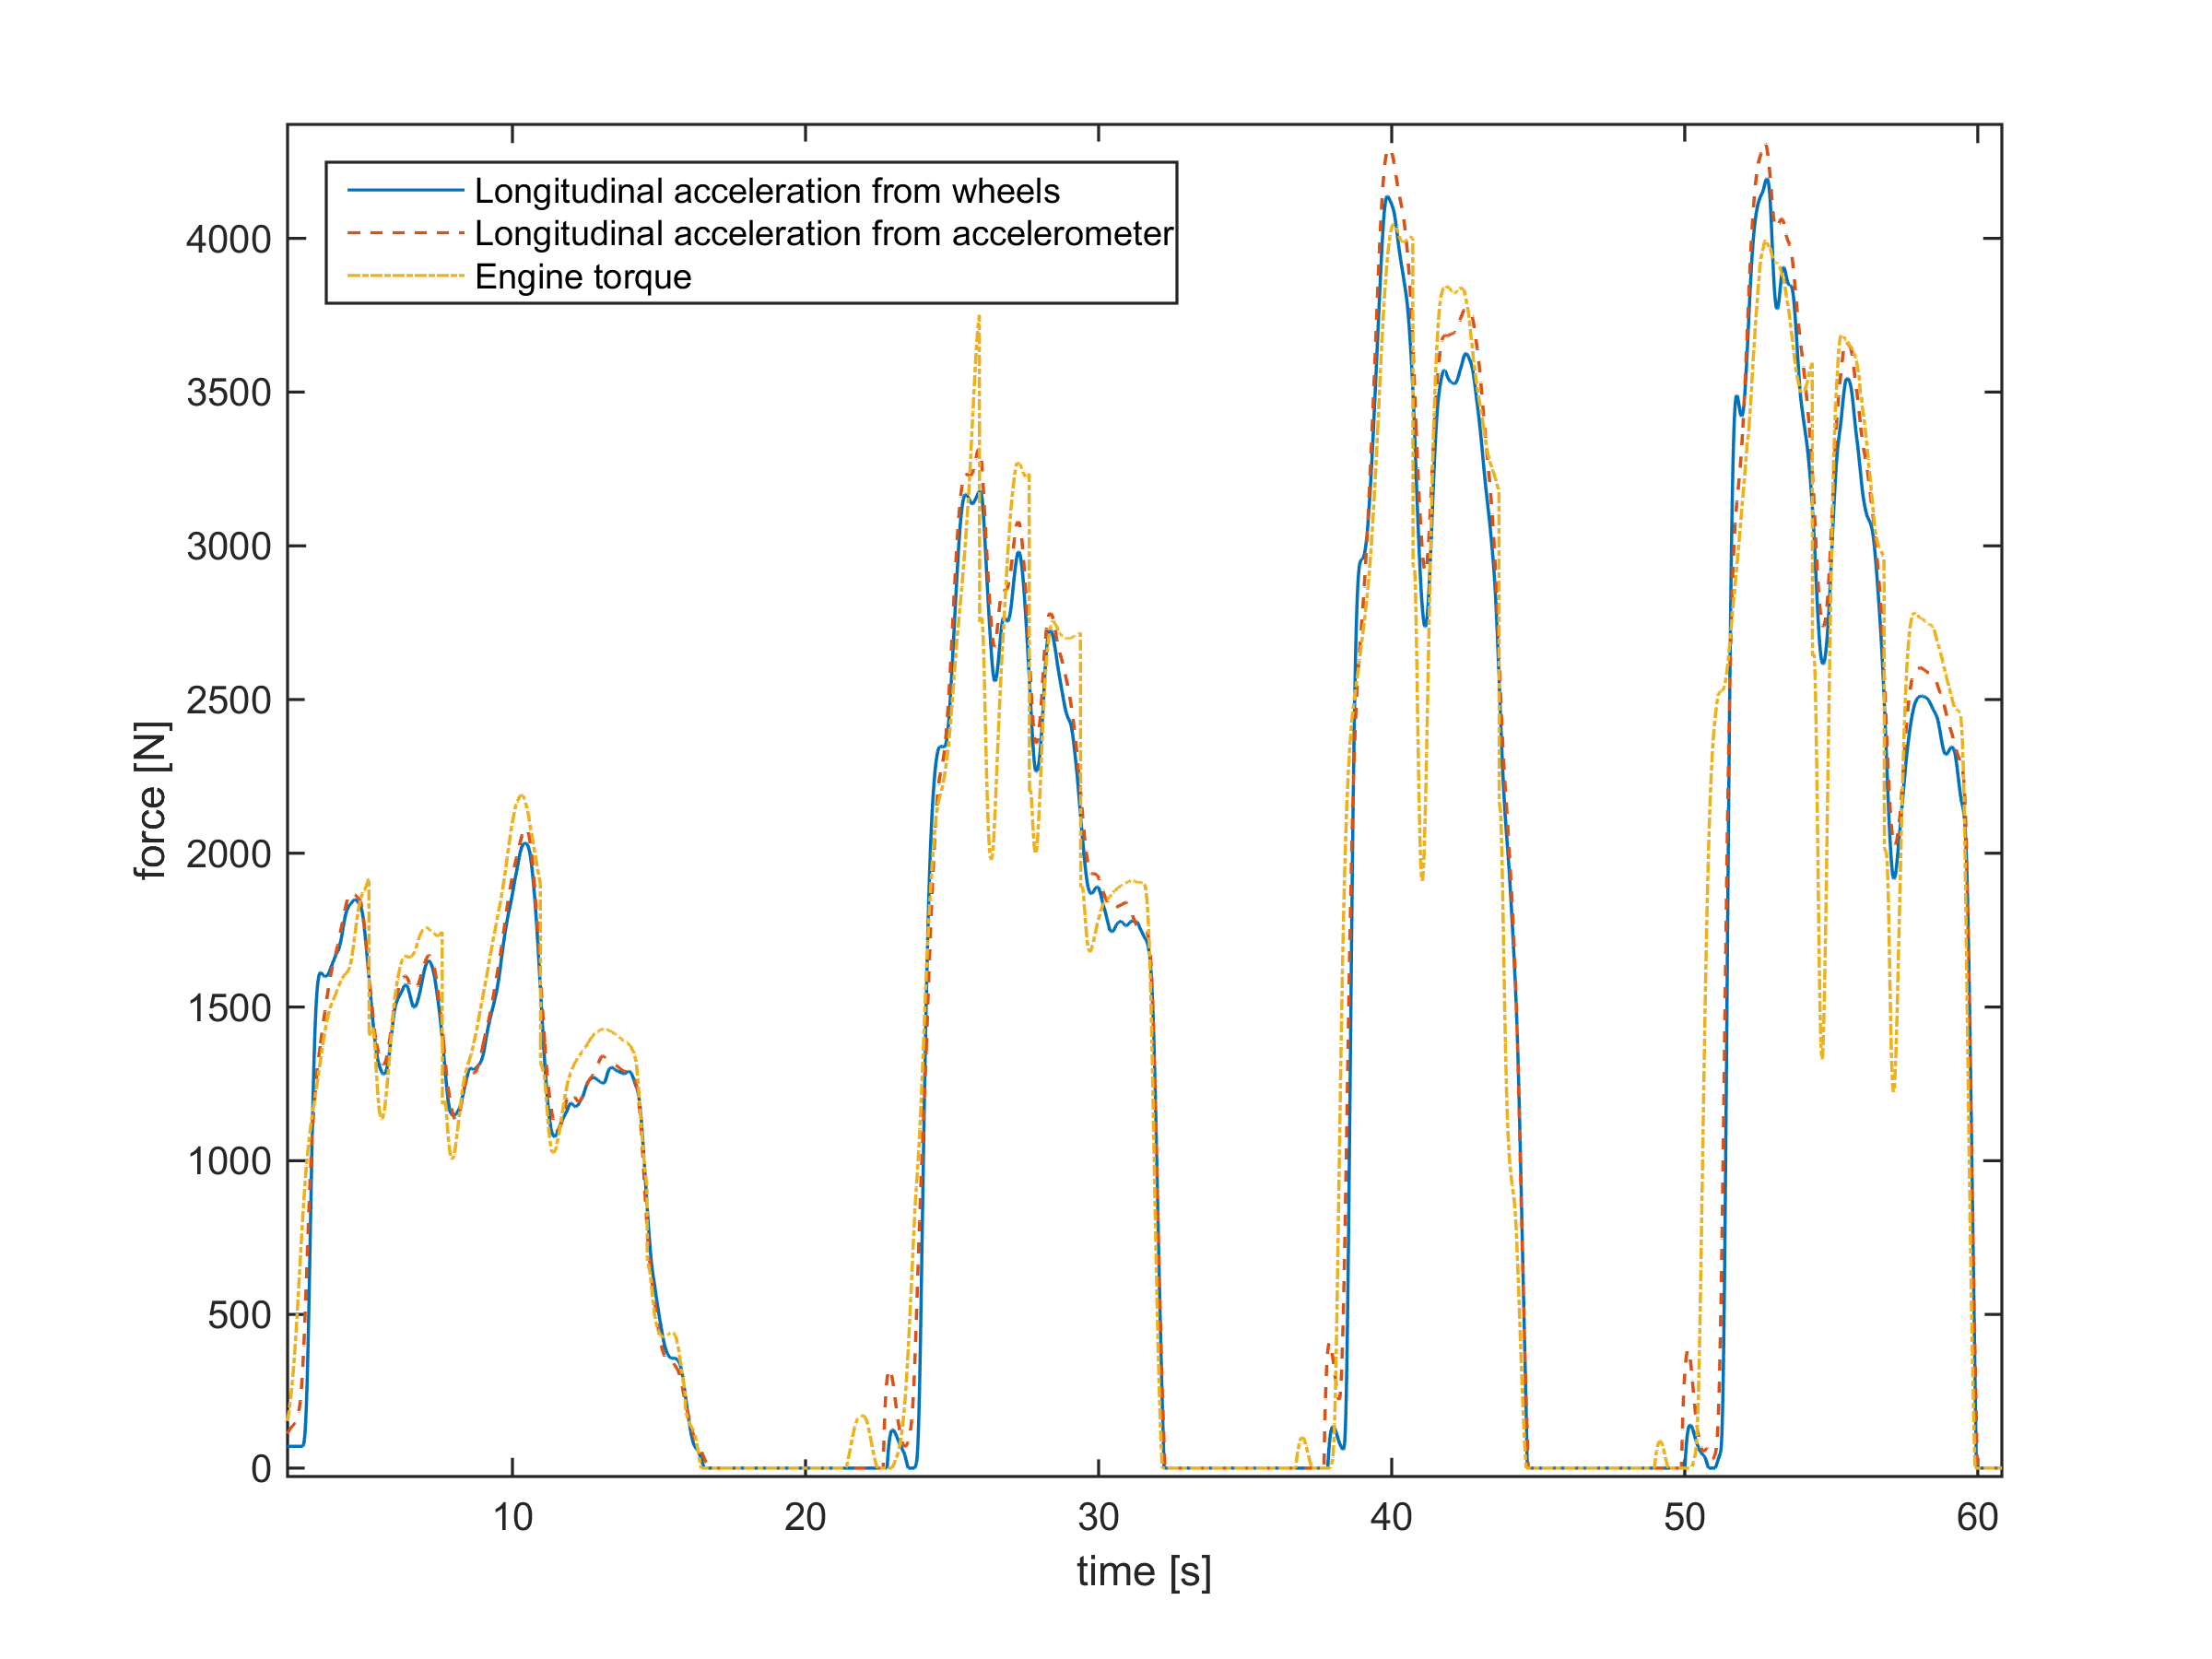
\includegraphics[width=1\textwidth]{Pictures/vehicle_model_comp_olikaacc}
	\caption{The vehicle force for the three different models while driving in a straight line on a flat road.}
	\label{vehicle_model_comp_olikaacc}
\end{figure}

The models will differ more when cornering, as can be seen in Figure \ref{vehicle_model_comp_race}. Neither the acceleration calculated from the undriven wheel speed or the measured acceleration from the accelerometer will be true while cornering. This is because both solutions for acquiring the vehicle acceleration is for longitudinal acceleration only. The undriven wheels is in this case the rear wheels and since these can't turn only the longitudinal acceleration is represented. The same goes for the accelerometer, only the longitudinal part of the acceleration is measured. The actual acceleration of the vehicle while cornering is a combination of longitudinal and lateral acceleration. The result of all this is that the force from the acceleration based vehicle models gets to low when cornering. 

\begin{figure}[h]
	\centering
	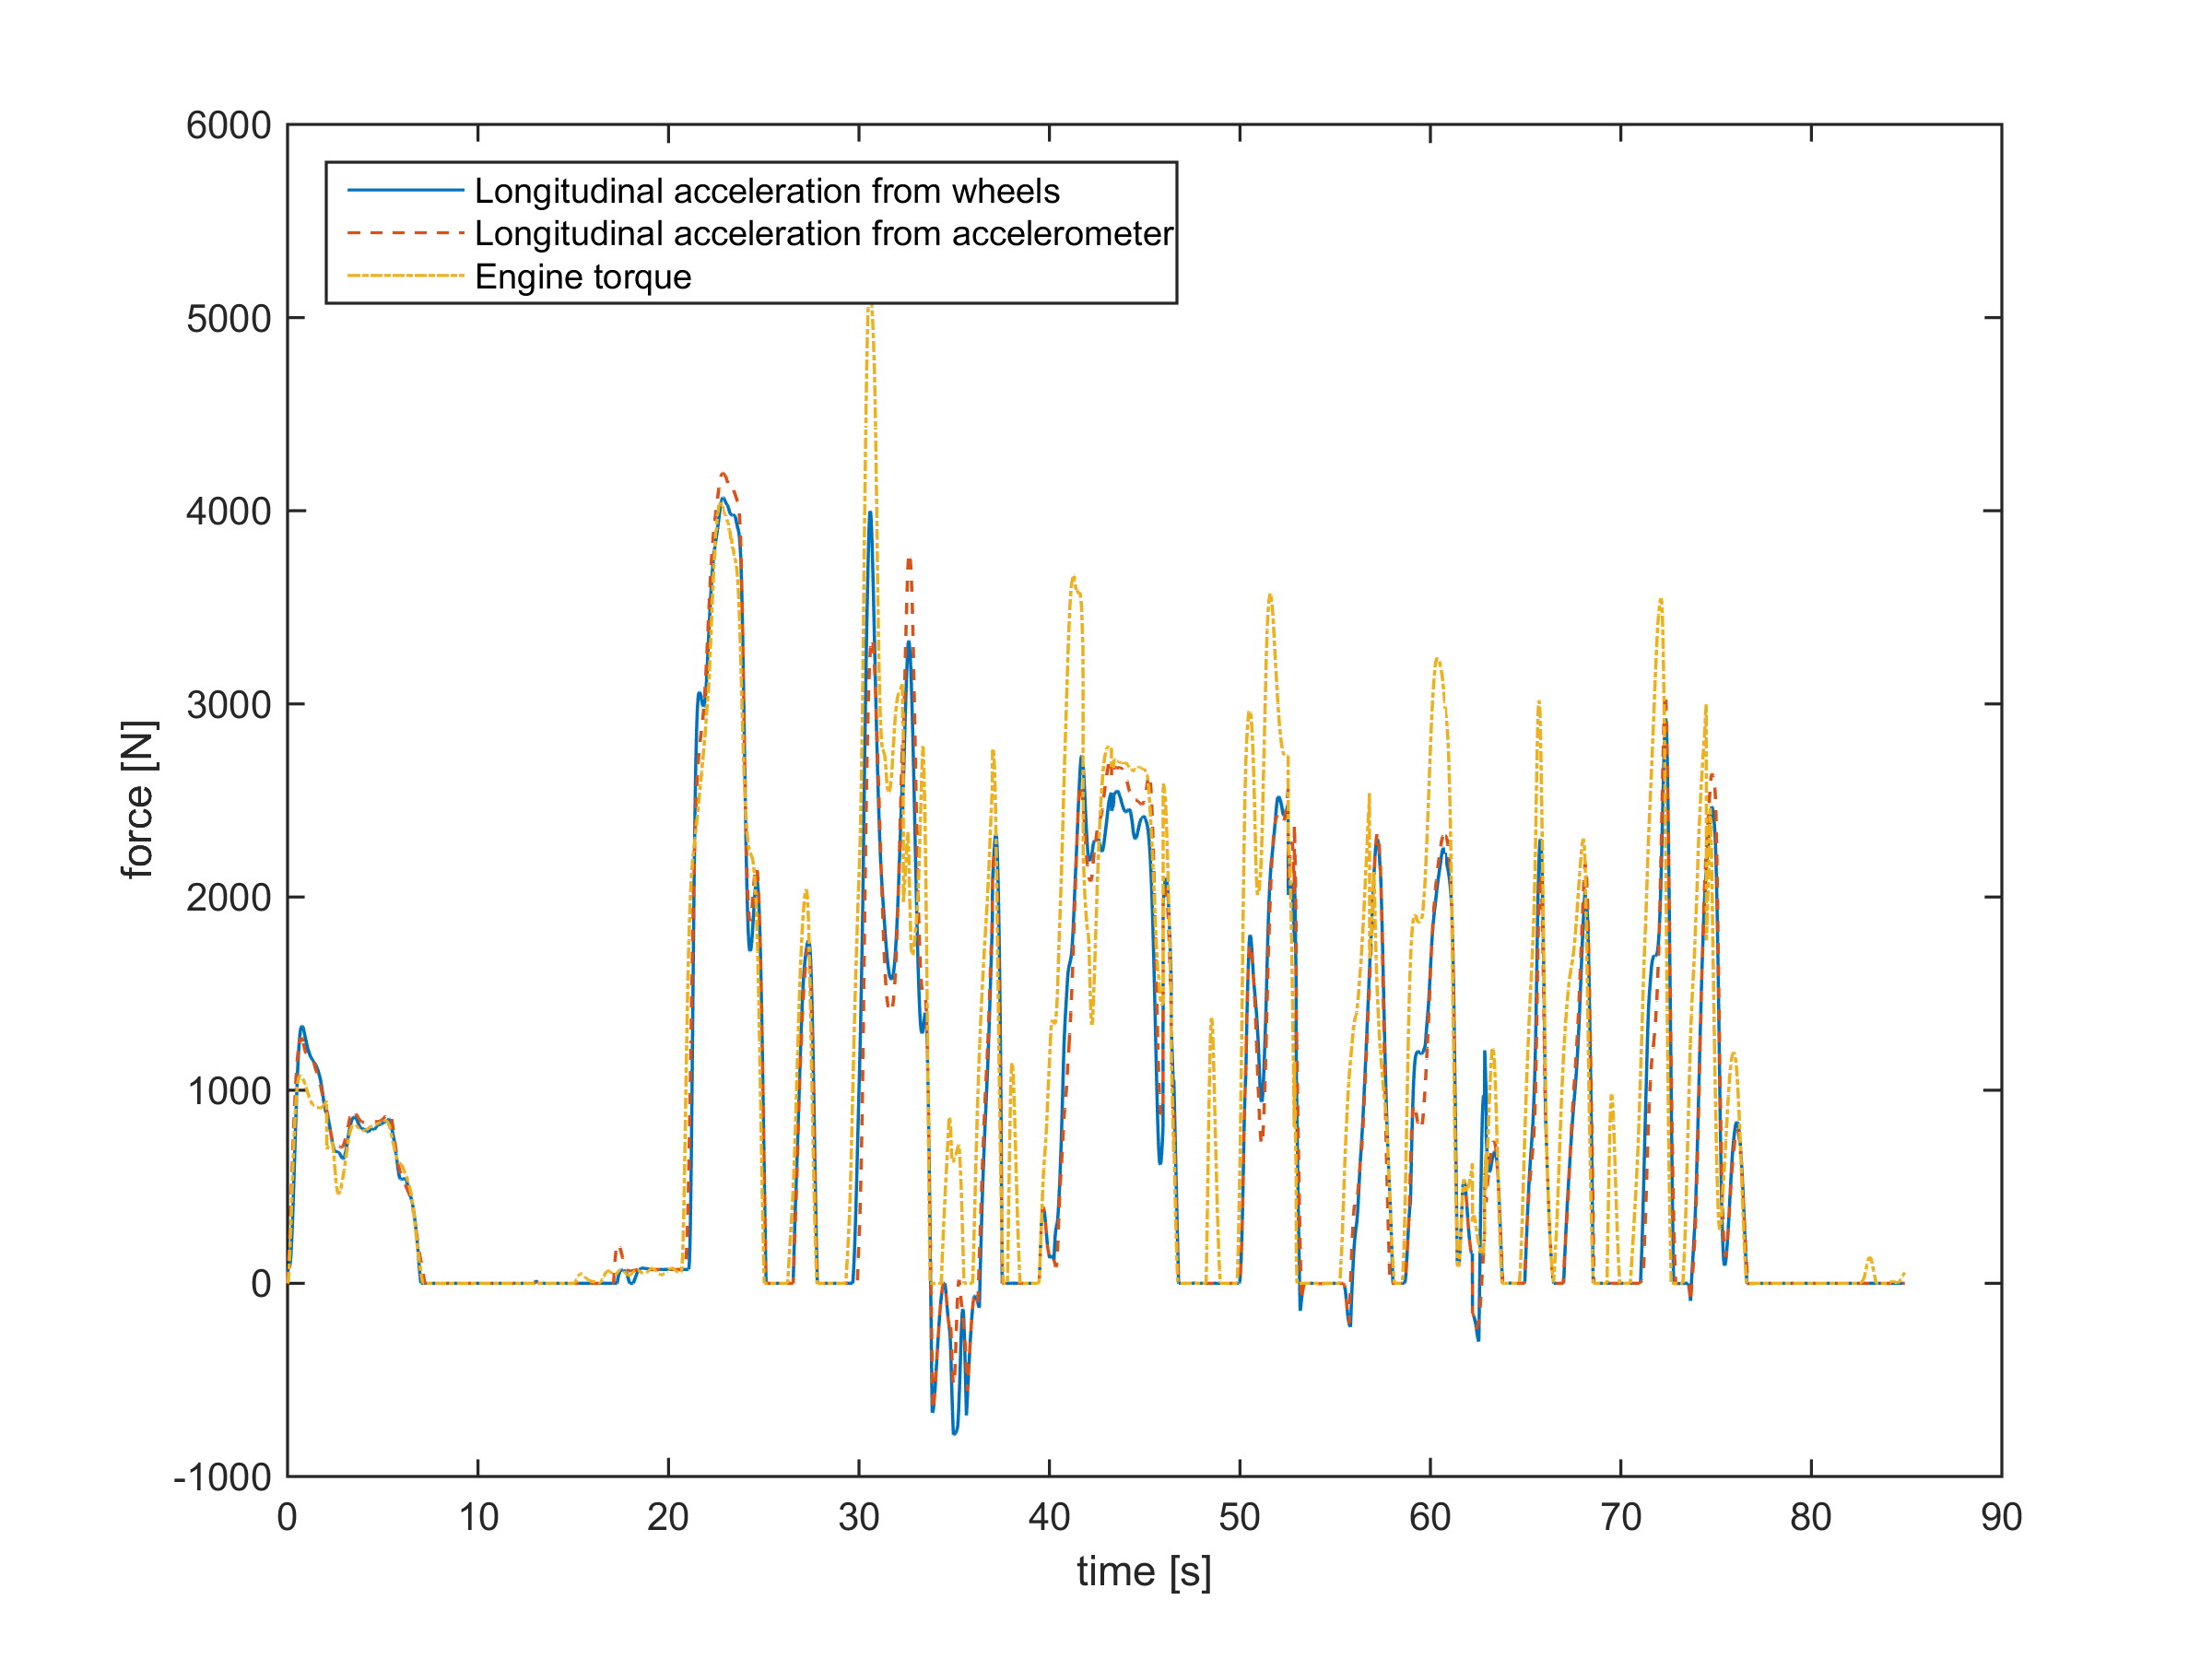
\includegraphics[width=1\textwidth]{Pictures/vehicle_model_comp_race}
	\caption{The vehicle force for the three different models while driving along a track with several corners.}
	\label{vehicle_model_comp_race}
\end{figure}

A solution to this could be to measure both the longitudinal and lateral accelerations with accelerometers and calculate the total acceleration of the vehicle. Unfortunately it's not that easy. When using both longitudinal and lateral acceleration of the vehicle the tire models must be able to account for both longitudinal and lateral force which is hard to model. More on this in Section \ref{tire_forces}.

It get's even worse when driving on a road that's hilly, as can be seen in Figure \ref{vehicle_model_comp_mm2}. While driving uphill or downhill the longitudinal acceleration from both the calculations and the accelerator measurements will be wrong. \todo{still no sure of this} The drive session shown is uphill, hence the force will be to low since the force needed to counter the force of gravity isn't considered. When cornering both acceleration based models where almost equally faulty at all time. When driving in a hill there's a difference between them. This is because the model based on undriven wheel acceleration won't consider the force of gravity at all. The model based on the accelerometer will consider it to some extent since the accelerometer will incline with the car, although, it won't be right.

The acceleration based vehicle models have been discussed a lot so far. The model based on engine torque hasn't been mentioned much at all and it has even been implied that this one is correct when the acceleration based models are falling behind. This is because it really is a good model that fills it purpose. 

\begin{figure}[h]
	\centering
	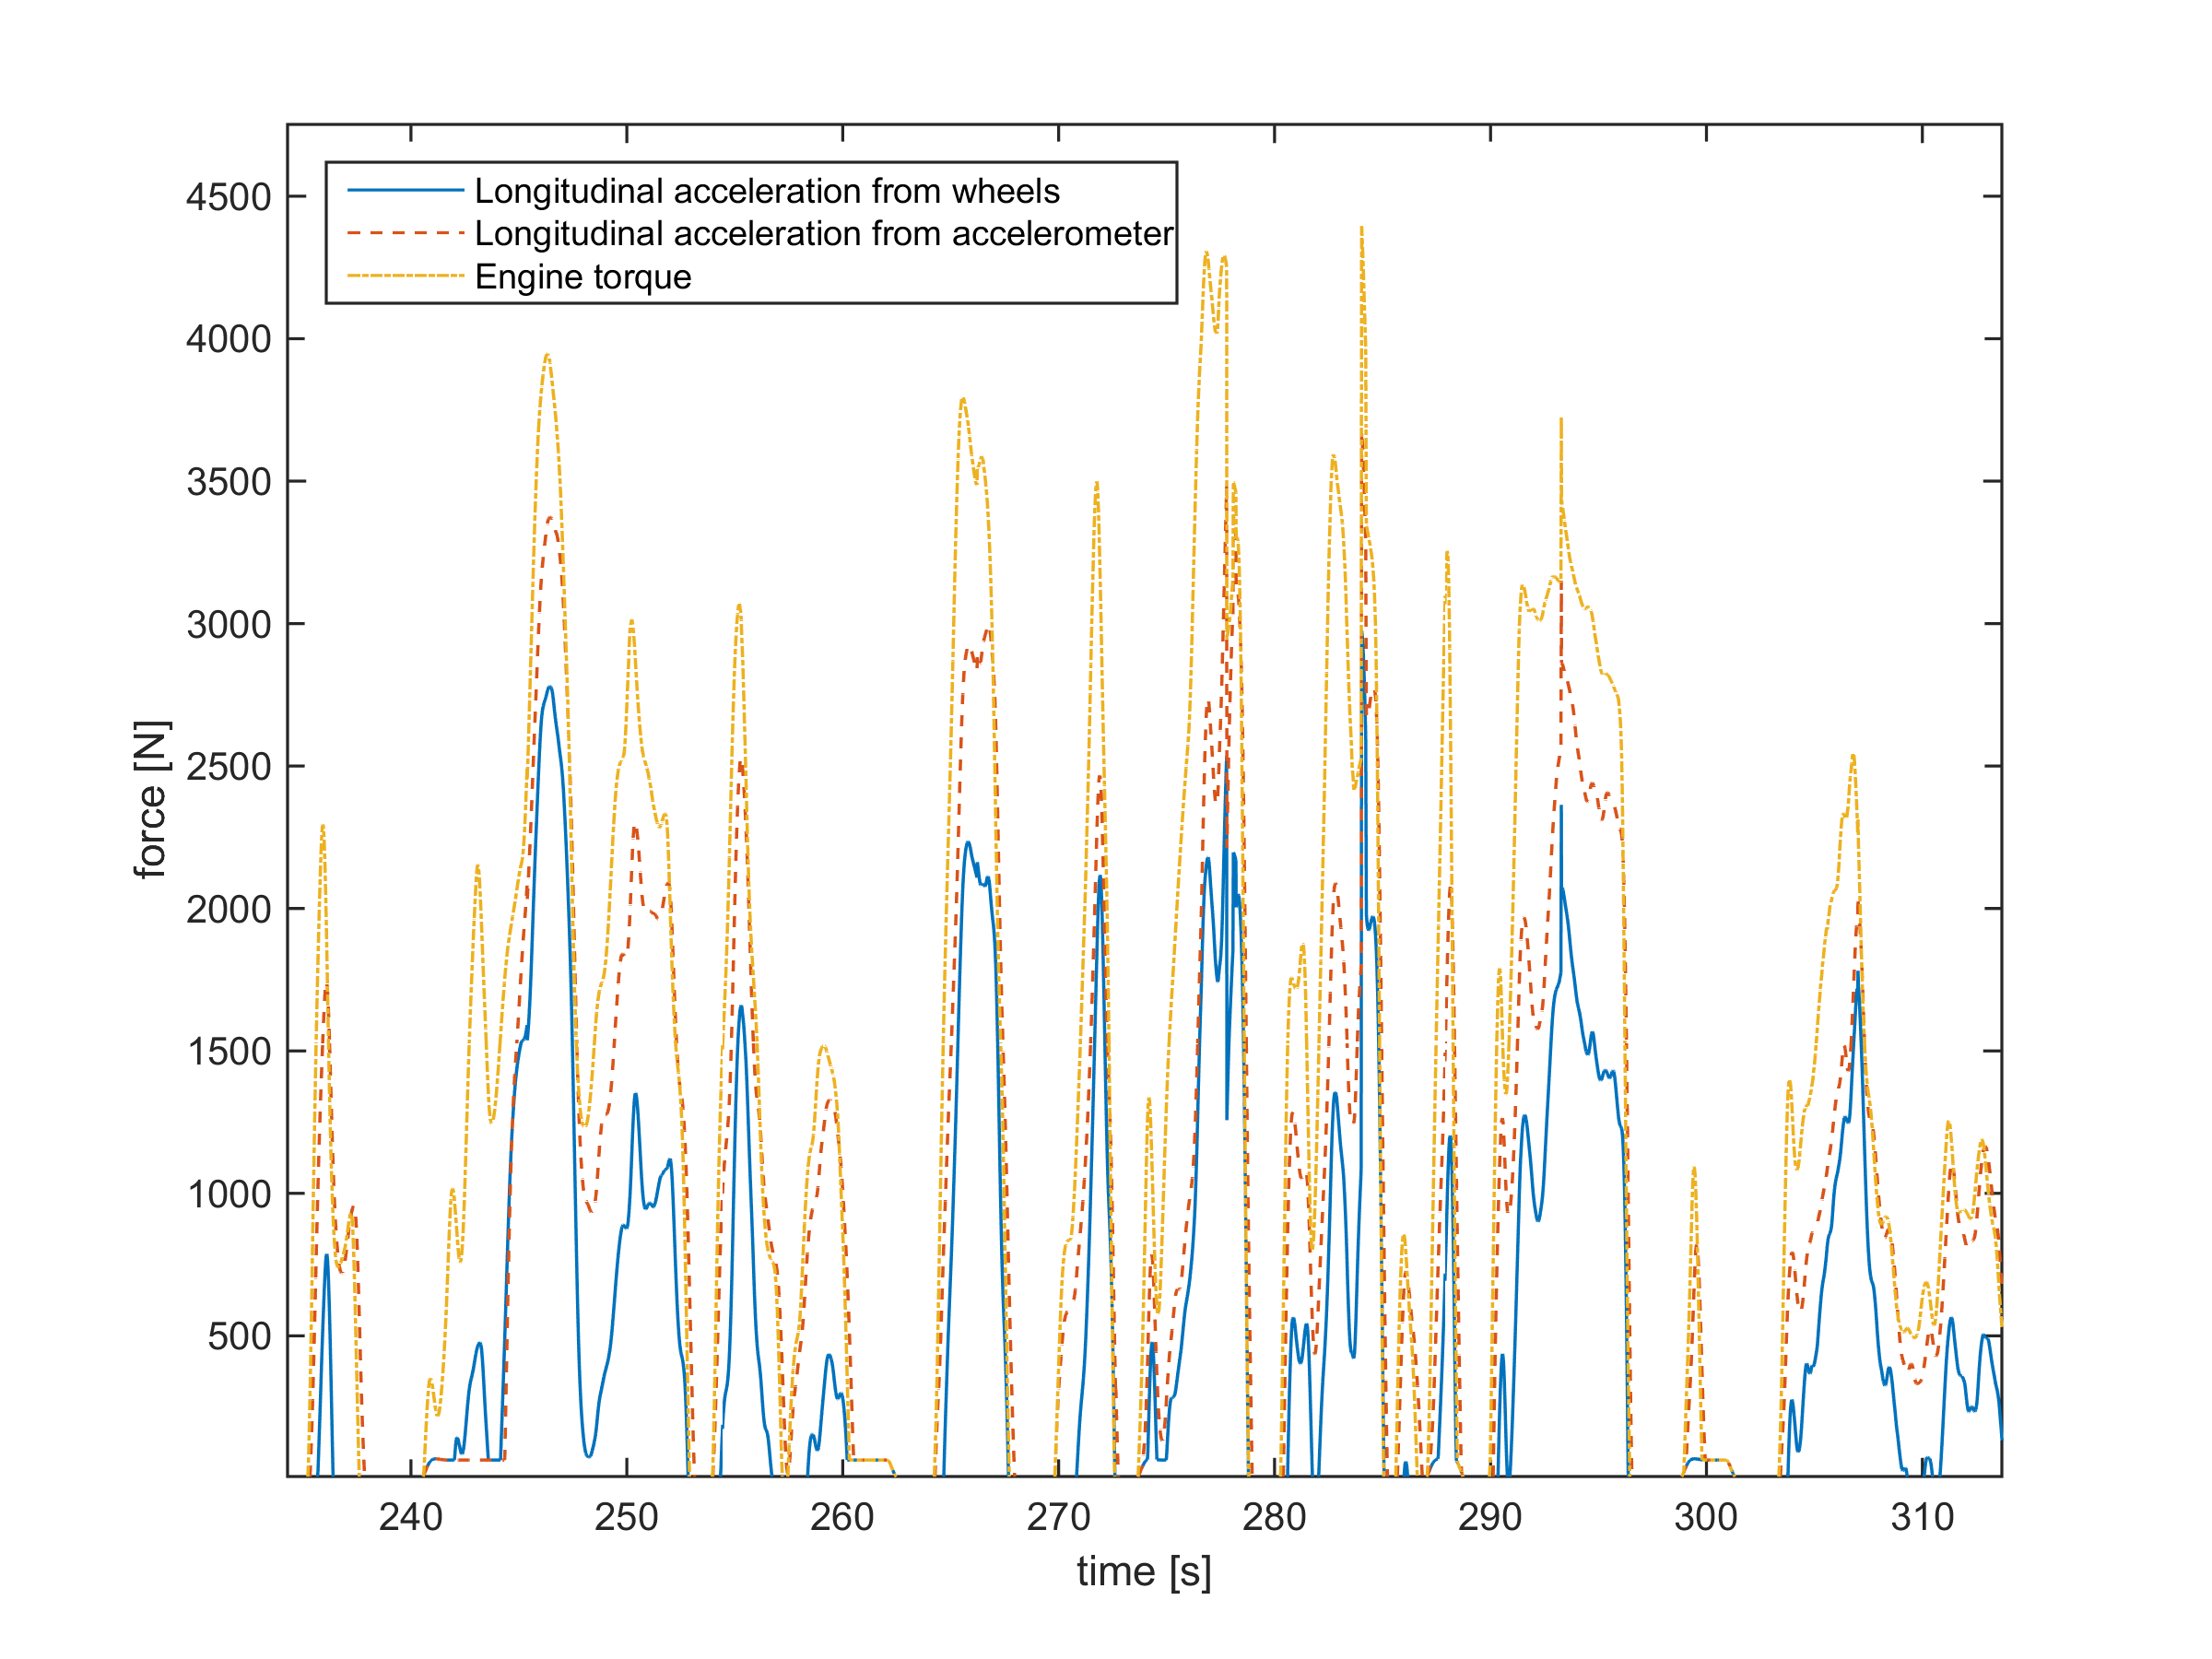
\includegraphics[width=1\textwidth]{Pictures/vehicle_model_comp_mm2}
	\caption{The vehicle force for the three different models while driving along a track with several corners and hills.}
	\label{vehicle_model_comp_mm2}
\end{figure}



\section{Tire forces}
\label{tire_forces}
The characteristic of a tire is very complex, which makes the actual force generated to the vehicle difficult to obtain. As was shown in the theory part (\ref{sec:tire_models}) there are several tire models that can be used, everyone of them with different properties.

A tire can generate both longitudinal and lateral force. It's quite easy to create a tire model that considers both these forces, the hard part is to acquire all the input parameters to the model in real time while driving. The parameters to model the lateral force are especially hard to obtain. These parameters are the slip angle and the lateral tire stiffness. Since these are so hard to calculate only the longitudinal part of a force model is used. The main dynamic parameters of a longitudinal tire force model (except Magic formula) includes the slip ratio, normal force, and the tire/road friction coefficient. A fourth, less dynamic parameter is the longitudinal tire stiffness. 
\begin{equation}
F_{tire, longitudinal} = f(\kappa, Fz, \mu, C_{x})
\end{equation}
The slip ratio is calculated from the wheels difference in angular and forward velocity as seen in equation $ \ref{eq:longslip} $, the normal force from the weight of the vehicle and the changing weight distribution derived in \ref{normal_force}, and the tire stiffness as explained in \ref{sec:tire_stiffness}. Thereafter, the only dynamic parameter of the tire force equation becomes the friction coefficient. By choosing the correct $ \mu $, the force from the tire model will equal the force from the vehicle model. This calculation is done in a feedback manner, meaning that the tire force depends on the friction coefficient derived in the previous iteration.

\subsection{Choosing a tire model}
Four models where described in the theory part. Brush model, Dugoff model, Magic formula and a tire model created by Ola Nockhammar at Borg Warner AB, further on called Ola's model.

The magic formula was ruled out almost immediately since it's a too complicated model to be adaptive enough. It's great for simulating a specific tire in a lab for example but using it in a real time car environment won't work. It's just too many parameters to estimate when switching from summer to winter tires for example. \todo{hmm?}

The other three models are more simple with fewer input parameters and above all it's parameters that are more easily available, like slip ratio and normal force. The Brush model and the Dugoff model are even too simple. The only available parameter to change the characteristics of the slip/force curve is the longitudinal tire stiffness. Ola's model on the other hand contains two degrees of freedom by introducing a second parameter to affect the inclination of the slip/force curve. Hence, it's easier to model a tire correctly with this model. Another positive aspect is the fact that the model is made for longitudinal force estimation only. Thus, it doesn't need to be modified for longitudinal use only like the Brush and Dugoff models. \todo{is this true?}

All in all, Ola's model was the obvious choice for this work.

\subsection{Tire model parameters for Ola's tire model}
In this section the four model parameters that affects Ola's tire model will be explained in more detail.

\subsubsection{Tire stiffness}
The tire stiffness is obtained by deriving the tire force generated per slip for values around zero, i.e. the gradient of the slip/force curve at zero slip. The slip force curve for two different tire stiffnesses can be seen in \ref{different_cx}. The interpretation from this figure is that a tires stiffness is an essential parameter to have in order to model the tire force correctly. 

\begin{figure}[h]
	\centering
	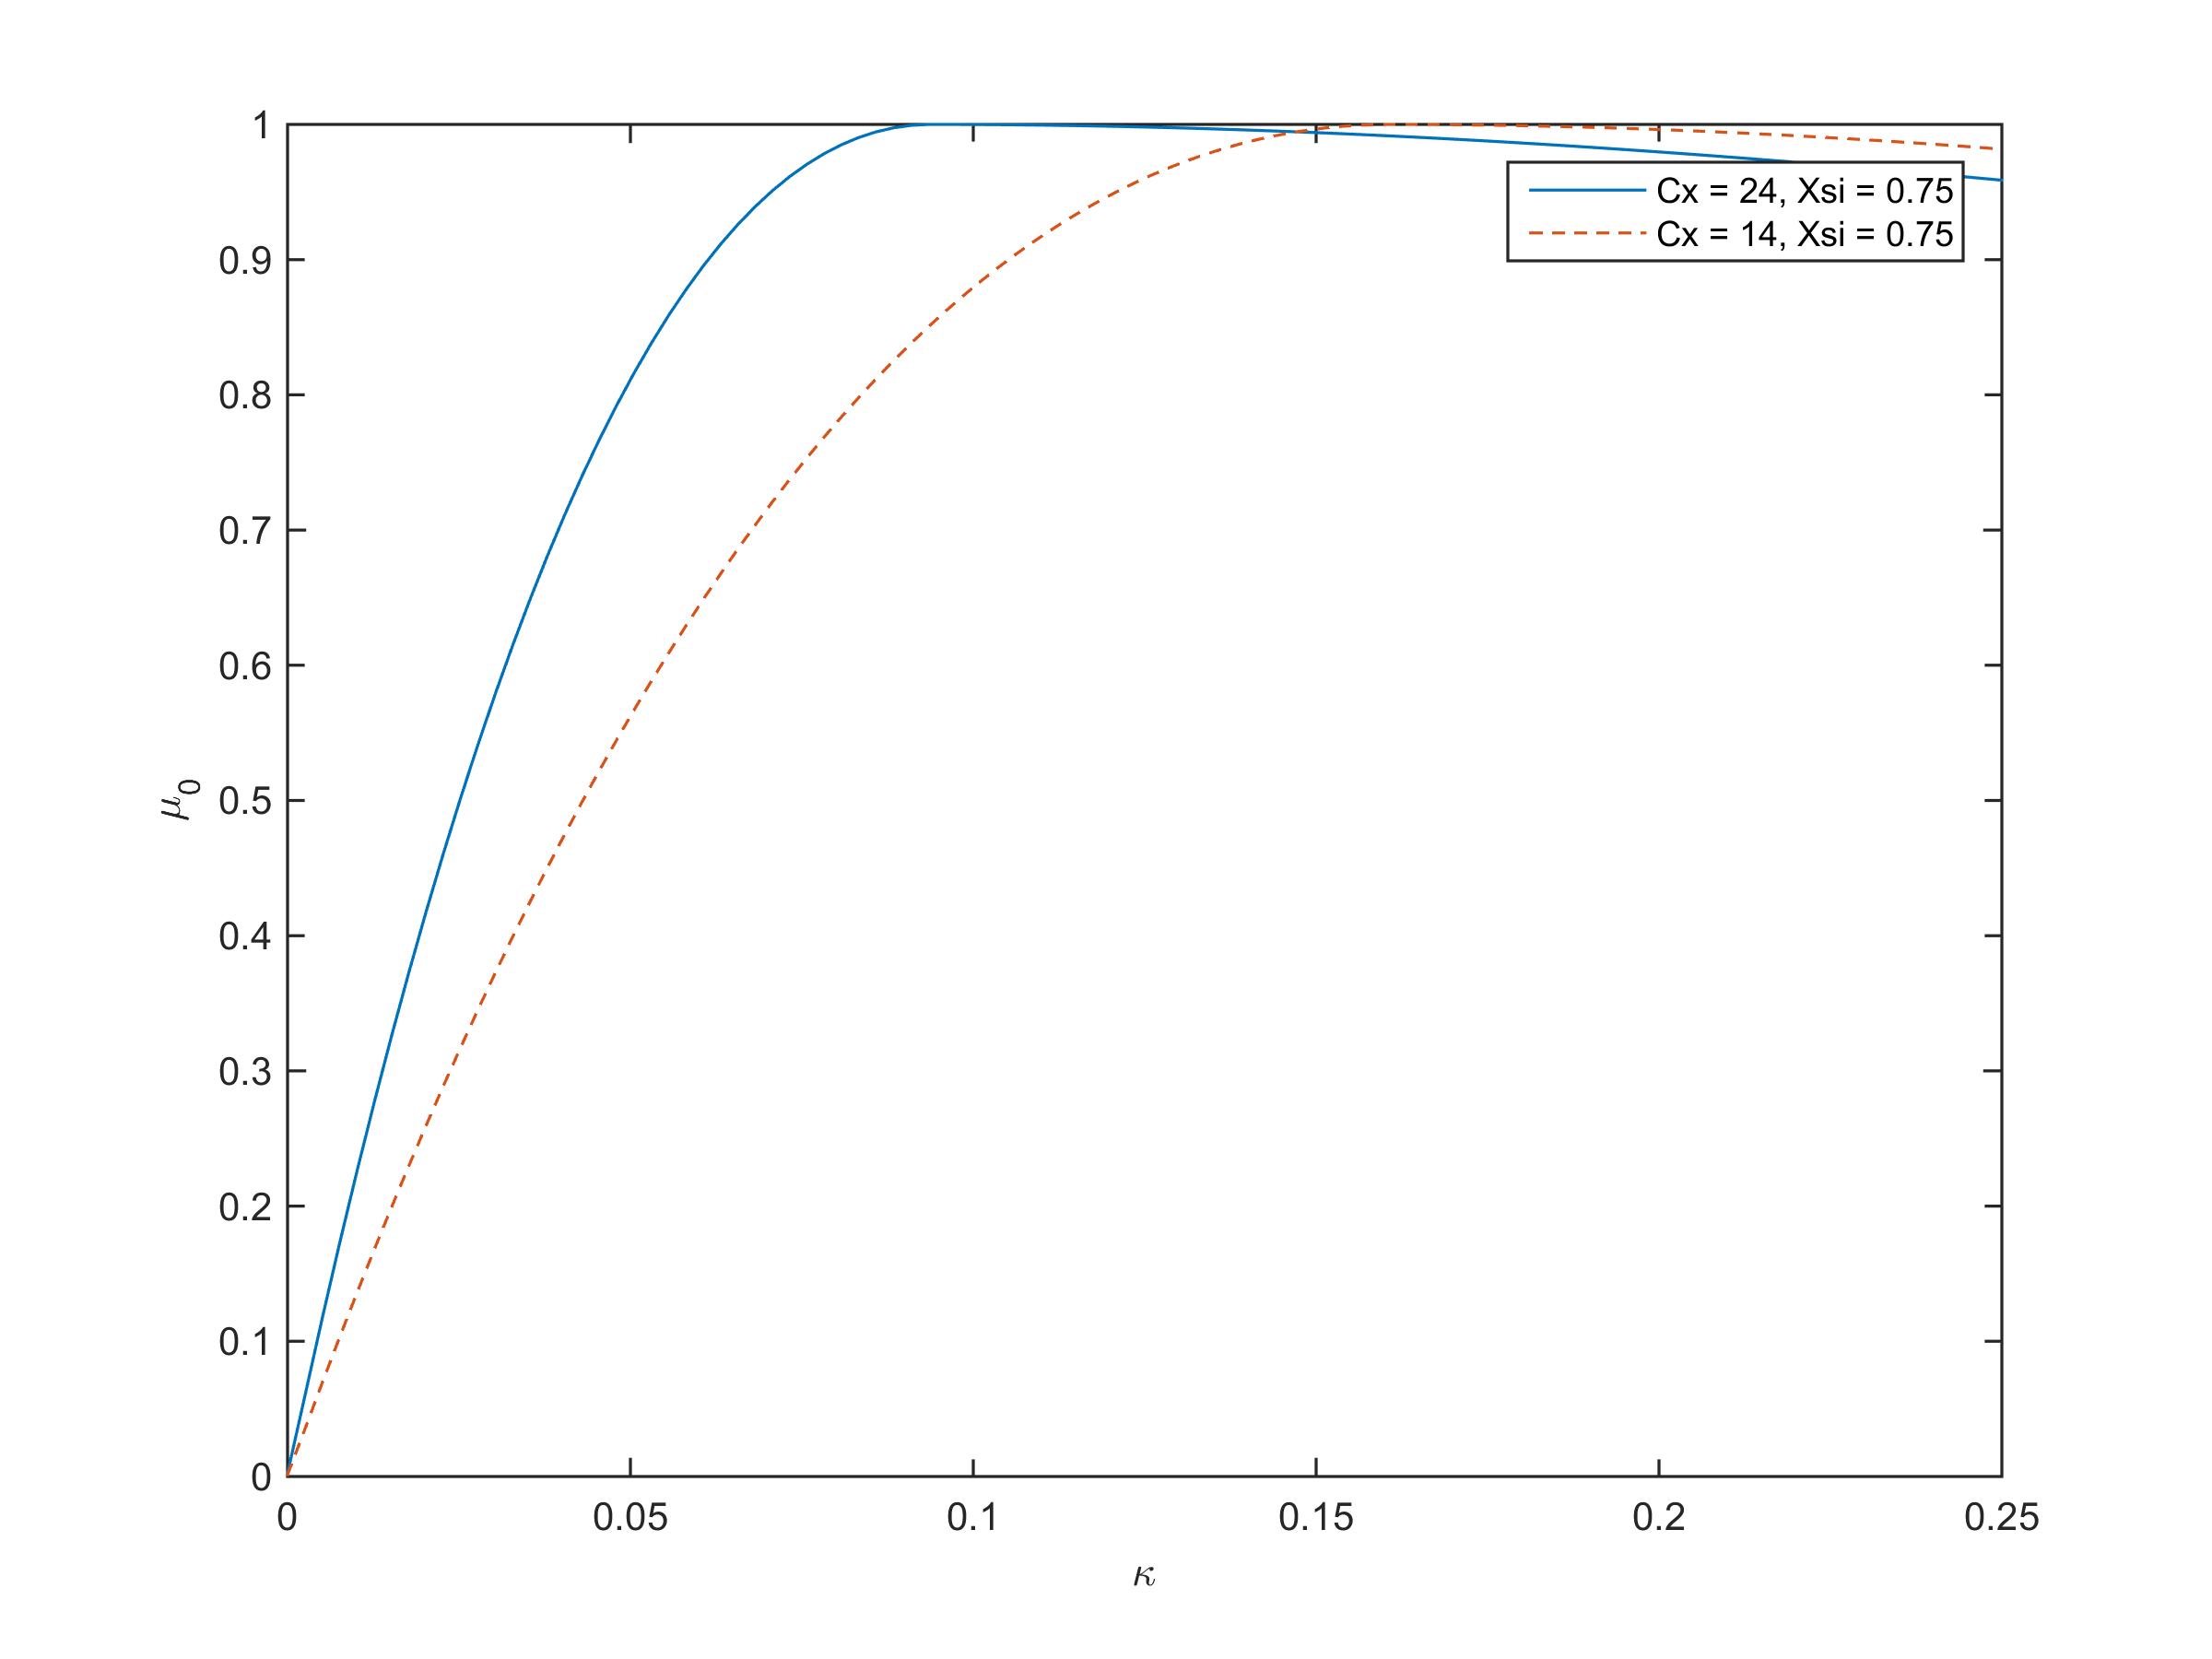
\includegraphics[width=0.8\textwidth]{Pictures/slipkraft_olika_cx}
	\caption {Normalized tire model force per slip ratio for different tire stiffnesses. $ \mu = 1.0 $.}
	\label{different_cx}
\end{figure}

Unfortunately, a tires characteristics is further complex, and cannot be explained by the tire stiffness as a parameter alone. Two different tires can have the same tire stiffness, but differing characteristics at larger slip ratio values. An example of this can be seen in \ref{different_xsi}. Generally, tires with lower tire stiffness value have higher $ \xi $, hence resulting in even lower forces for higher slip values.\todo{is this true?} Once again this is a good reason to use Ola's tire model since $ \xi $ can be modified in this model.

\begin{figure}[h]
	\centering
	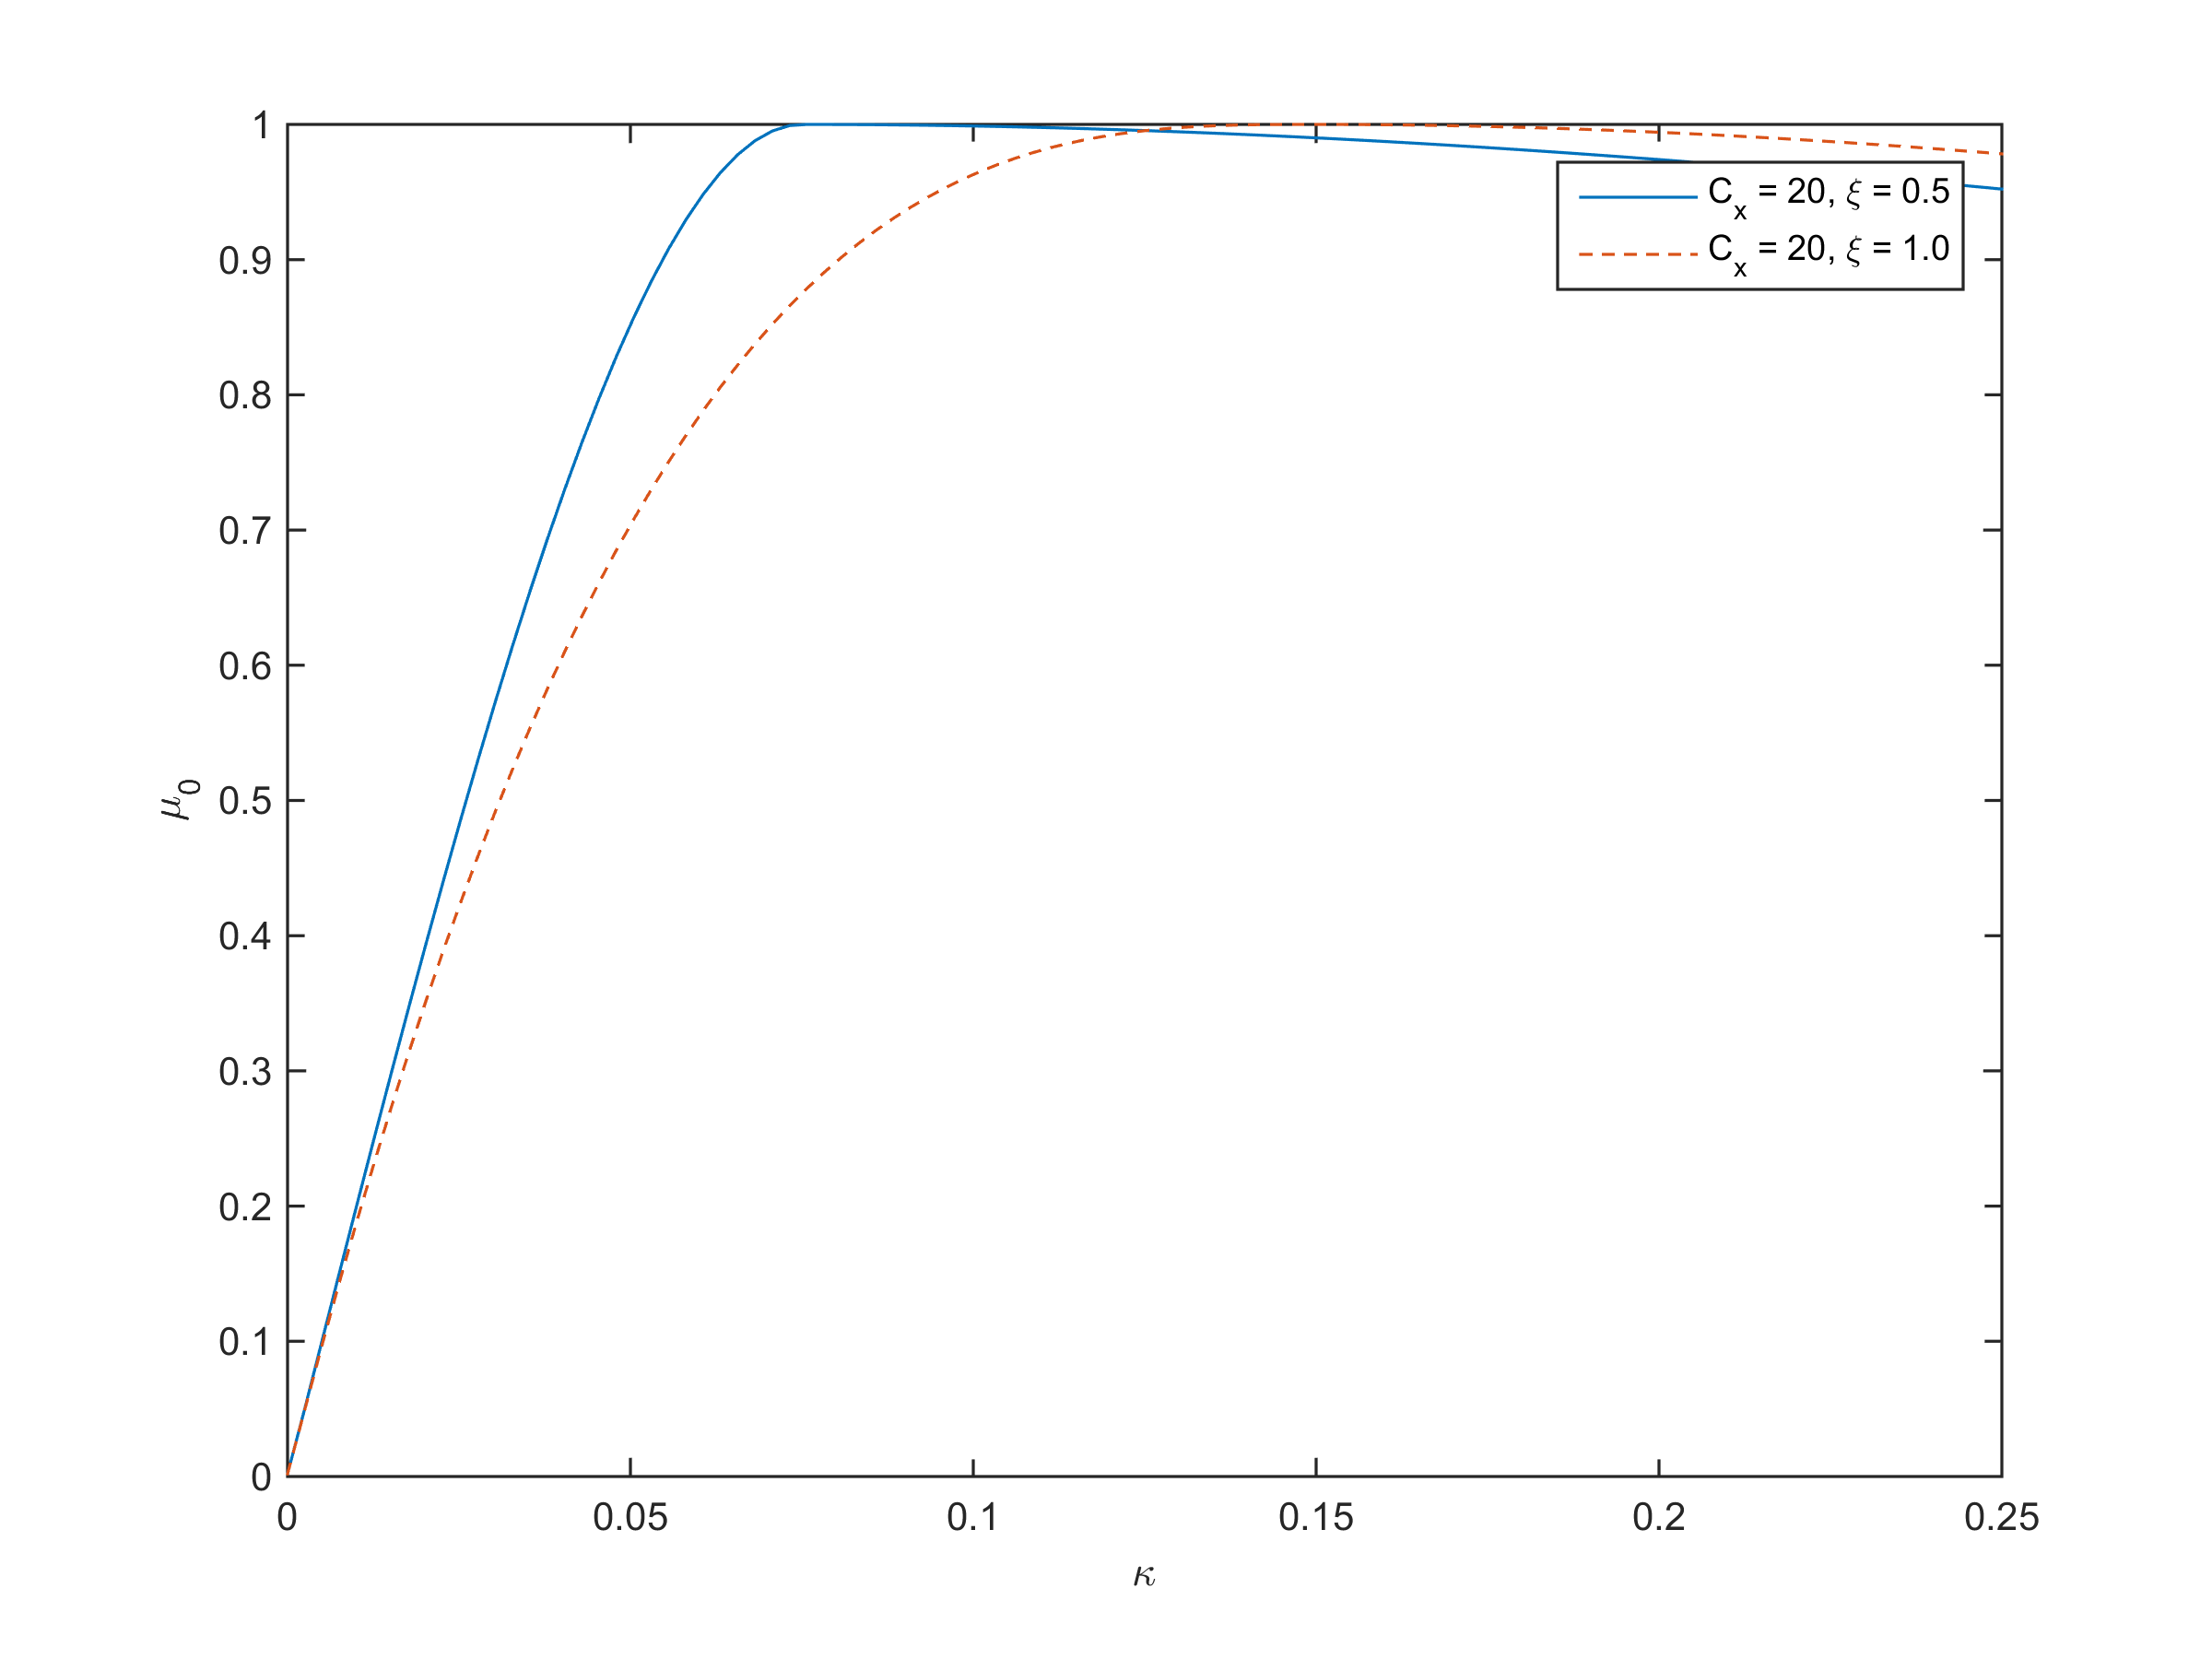
\includegraphics[width=0.8\textwidth]{Pictures/slipkraft_olika_xsi}
	\caption {Normalized tire model force per slip ratio for different tire characteristics for higher slip ratios.
		$ \mu = 1.0 $.}
	\label{different_xsi}
\end{figure}

The tire stiffness for a certain tire should theoretically be the same for different road surfaces. Nevertheless, testing has shown that the actual inclination of the slip/force curve for small slips can differ for different road surfaces. The tire stiffness therefore has to be compensated accordingly depending on the roads friction coefficient. \todo{this needs to be exaplained in more detail}

\subsubsection{Slip ratio}
As seen most slip/force figures, the maximum force will be generated at a specific slip and will thereafter decrease with an increasing slip ratio. If the tire model doesn't capture this force peak at the correct slip ratio value, it will become very difficult to match the tire model force with the calculated vehicle force. The slip ratio value during a real driving sequence is usually rather small (maximum force is generally obtained at a slip ratio $ \geq 12 \% $), which means that a small variances in the slip ratio calculations will have a large impact on the resulting force.

In order to calculate the slip ratios of the two front wheels, the four wheel speeds are gathered from the vehicles CAN bus. These signals generally include quite a lot of measurement and/or process noisy which thereafter leads to a noisy slip ratio calculation, as can be seen in the first row of figure \ref{wheel_speed_and_slip}. In order to overcome this noise and capture the actual value, the signals are run through a low pass filter. The wheel speeds will, even after filtering, have an oscillating attribute. When theses oscillations from the front and its respective rear wheel are not synchronized and with different magnitude, the calculated slip ratio will have rather large variation compared to its real value. This can be seen in the second row of figure \ref{wheel_speed_and_slip}, where the wheel speeds are run trough a relatively slow low pass filter, i.e. a low pass filter with a high cutoff frequency. Most of the measure and/or process noise is removed, but due to the characteristics of the wheel speed sensor and its design, the signal will still oscillate with a frequency that is proportional to its angular velocity. To minimize the error from the oscillations, the wheel speeds are filtered with a lower cutoff frequency, which can be seen in the third row of figure \ref{wheel_speed_and_slip}. 
\begin{figure}[h]
	\centering
	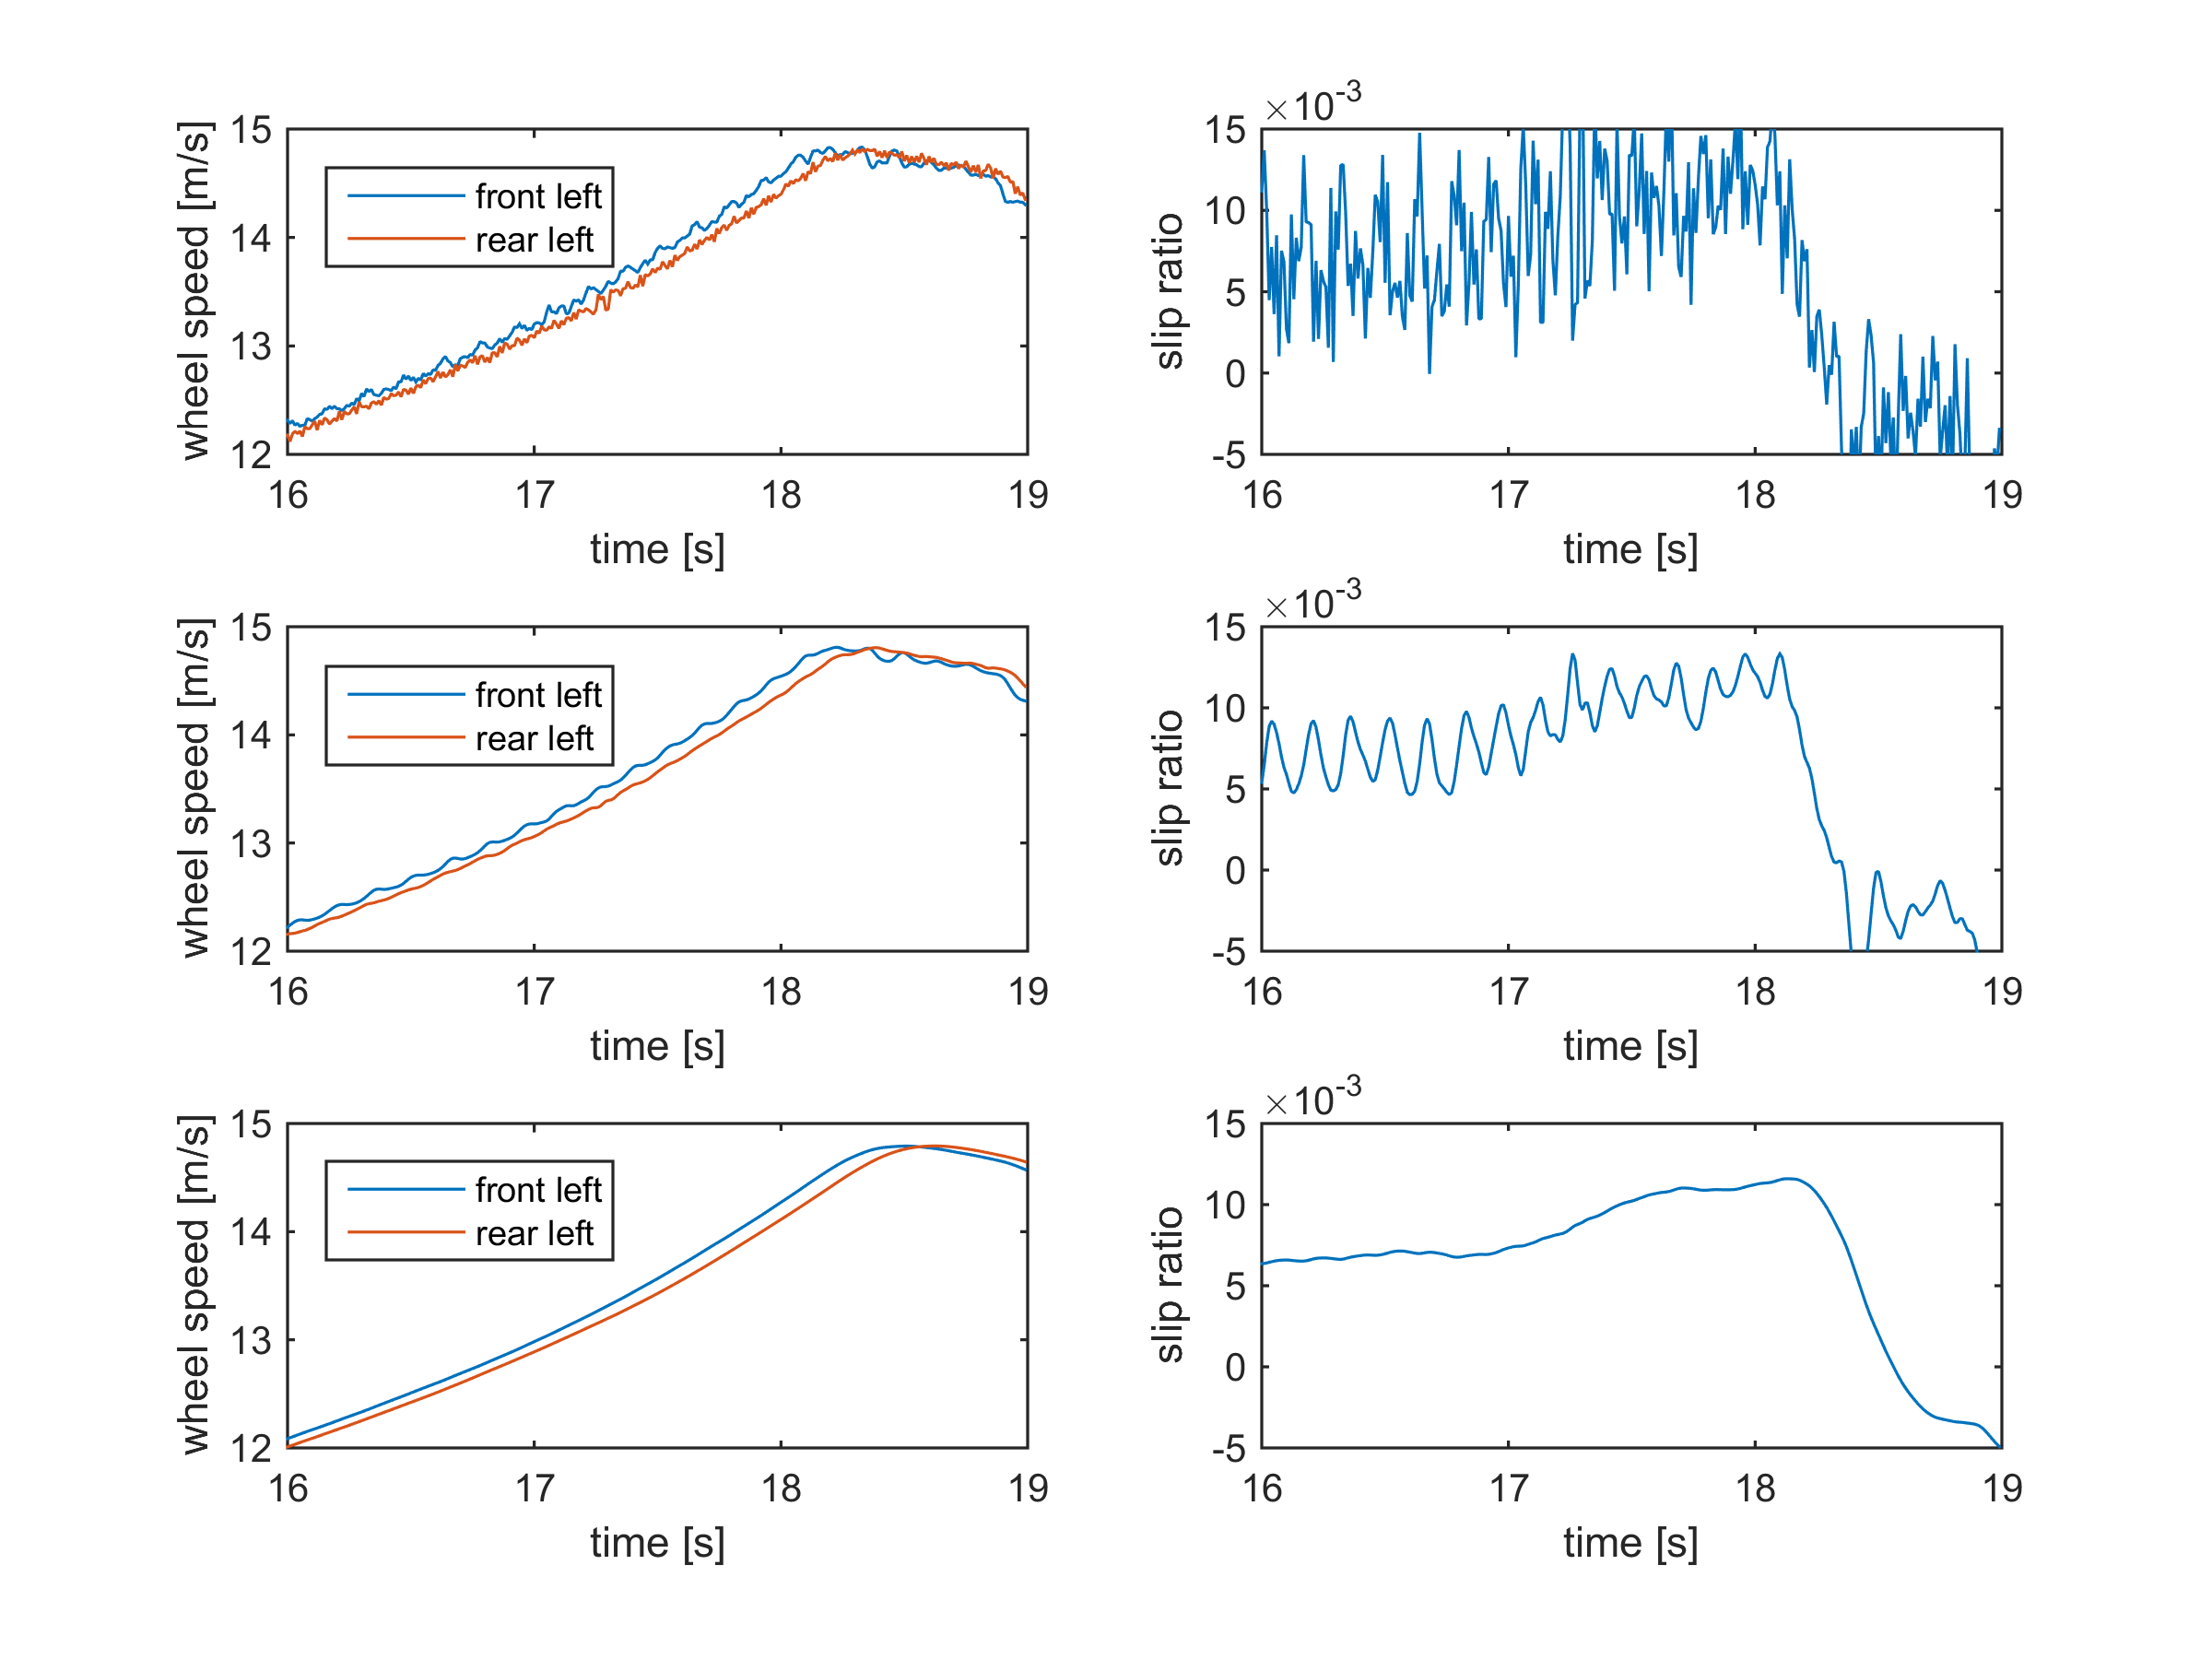
\includegraphics[width=1.0\textwidth]{Pictures/wheel_speed_and_slip}
	\caption {Wheel speeds and slips for different filters.}
	\label{wheel_speed_and_slip}
\end{figure}
Another concrete problem that arises when calculating the slip ratio, is that the radius for each wheel on a vehicle can be different, e.g. when the air pressure of a tire drops slightly over time. The wheel speed from the CAN bus will in this case be wrong, leading to a offset in the slip ratio calculations. \todo{explain more}

\todo{Skriva något fint om kraften med slip angle} The force/slip should be smaller when the slip angle is larger. In other words, when we have more lateral force, the longitudinal force will be smaller.

\subsubsection{Normal force}
The amount of longitudinal force (neglecting lateral forces) generated from a tire depends on the normal force acting on the tire. The force generated by a tire is linearly proportional to the normal force on the tire:
\begin{equation}
	F_{x} = F_{z}\mu_{0}
\end{equation}
Where the normalized force $ \mu_{0} $, never can exceed the friction coefficient between the tire and the road:
\begin{equation}
	\mu_{0} \leq \mu
\end{equation}
It is therefore important to know the loaded weight on each tire at every instant. This is done by the dynamic weight distribution calculations explained in section \ref{normal_force}. These calculations are rather simplified, where the difference in chassis stiffness between front and back is not considered. These chassis stiffnesses are vehicle specific and hard to estimate. 

This means that the maximum longitudinal force obtained by either the vehicle model or the tire force model, can never be larger than the normal force multiplied by the tire/road friction coefficient, which can be helpful to rule out unreasonable values. 

\subsubsection{Friction coefficient}
\label{section_friction coefficient}
The final dynamic parameter that affect the tire force model is the friction coefficient between the tire and the road. The friction coefficient decides the limit of the normalized force that can be generated through the tires, and therefore in the 

\begin{figure}[h]
	\centering
	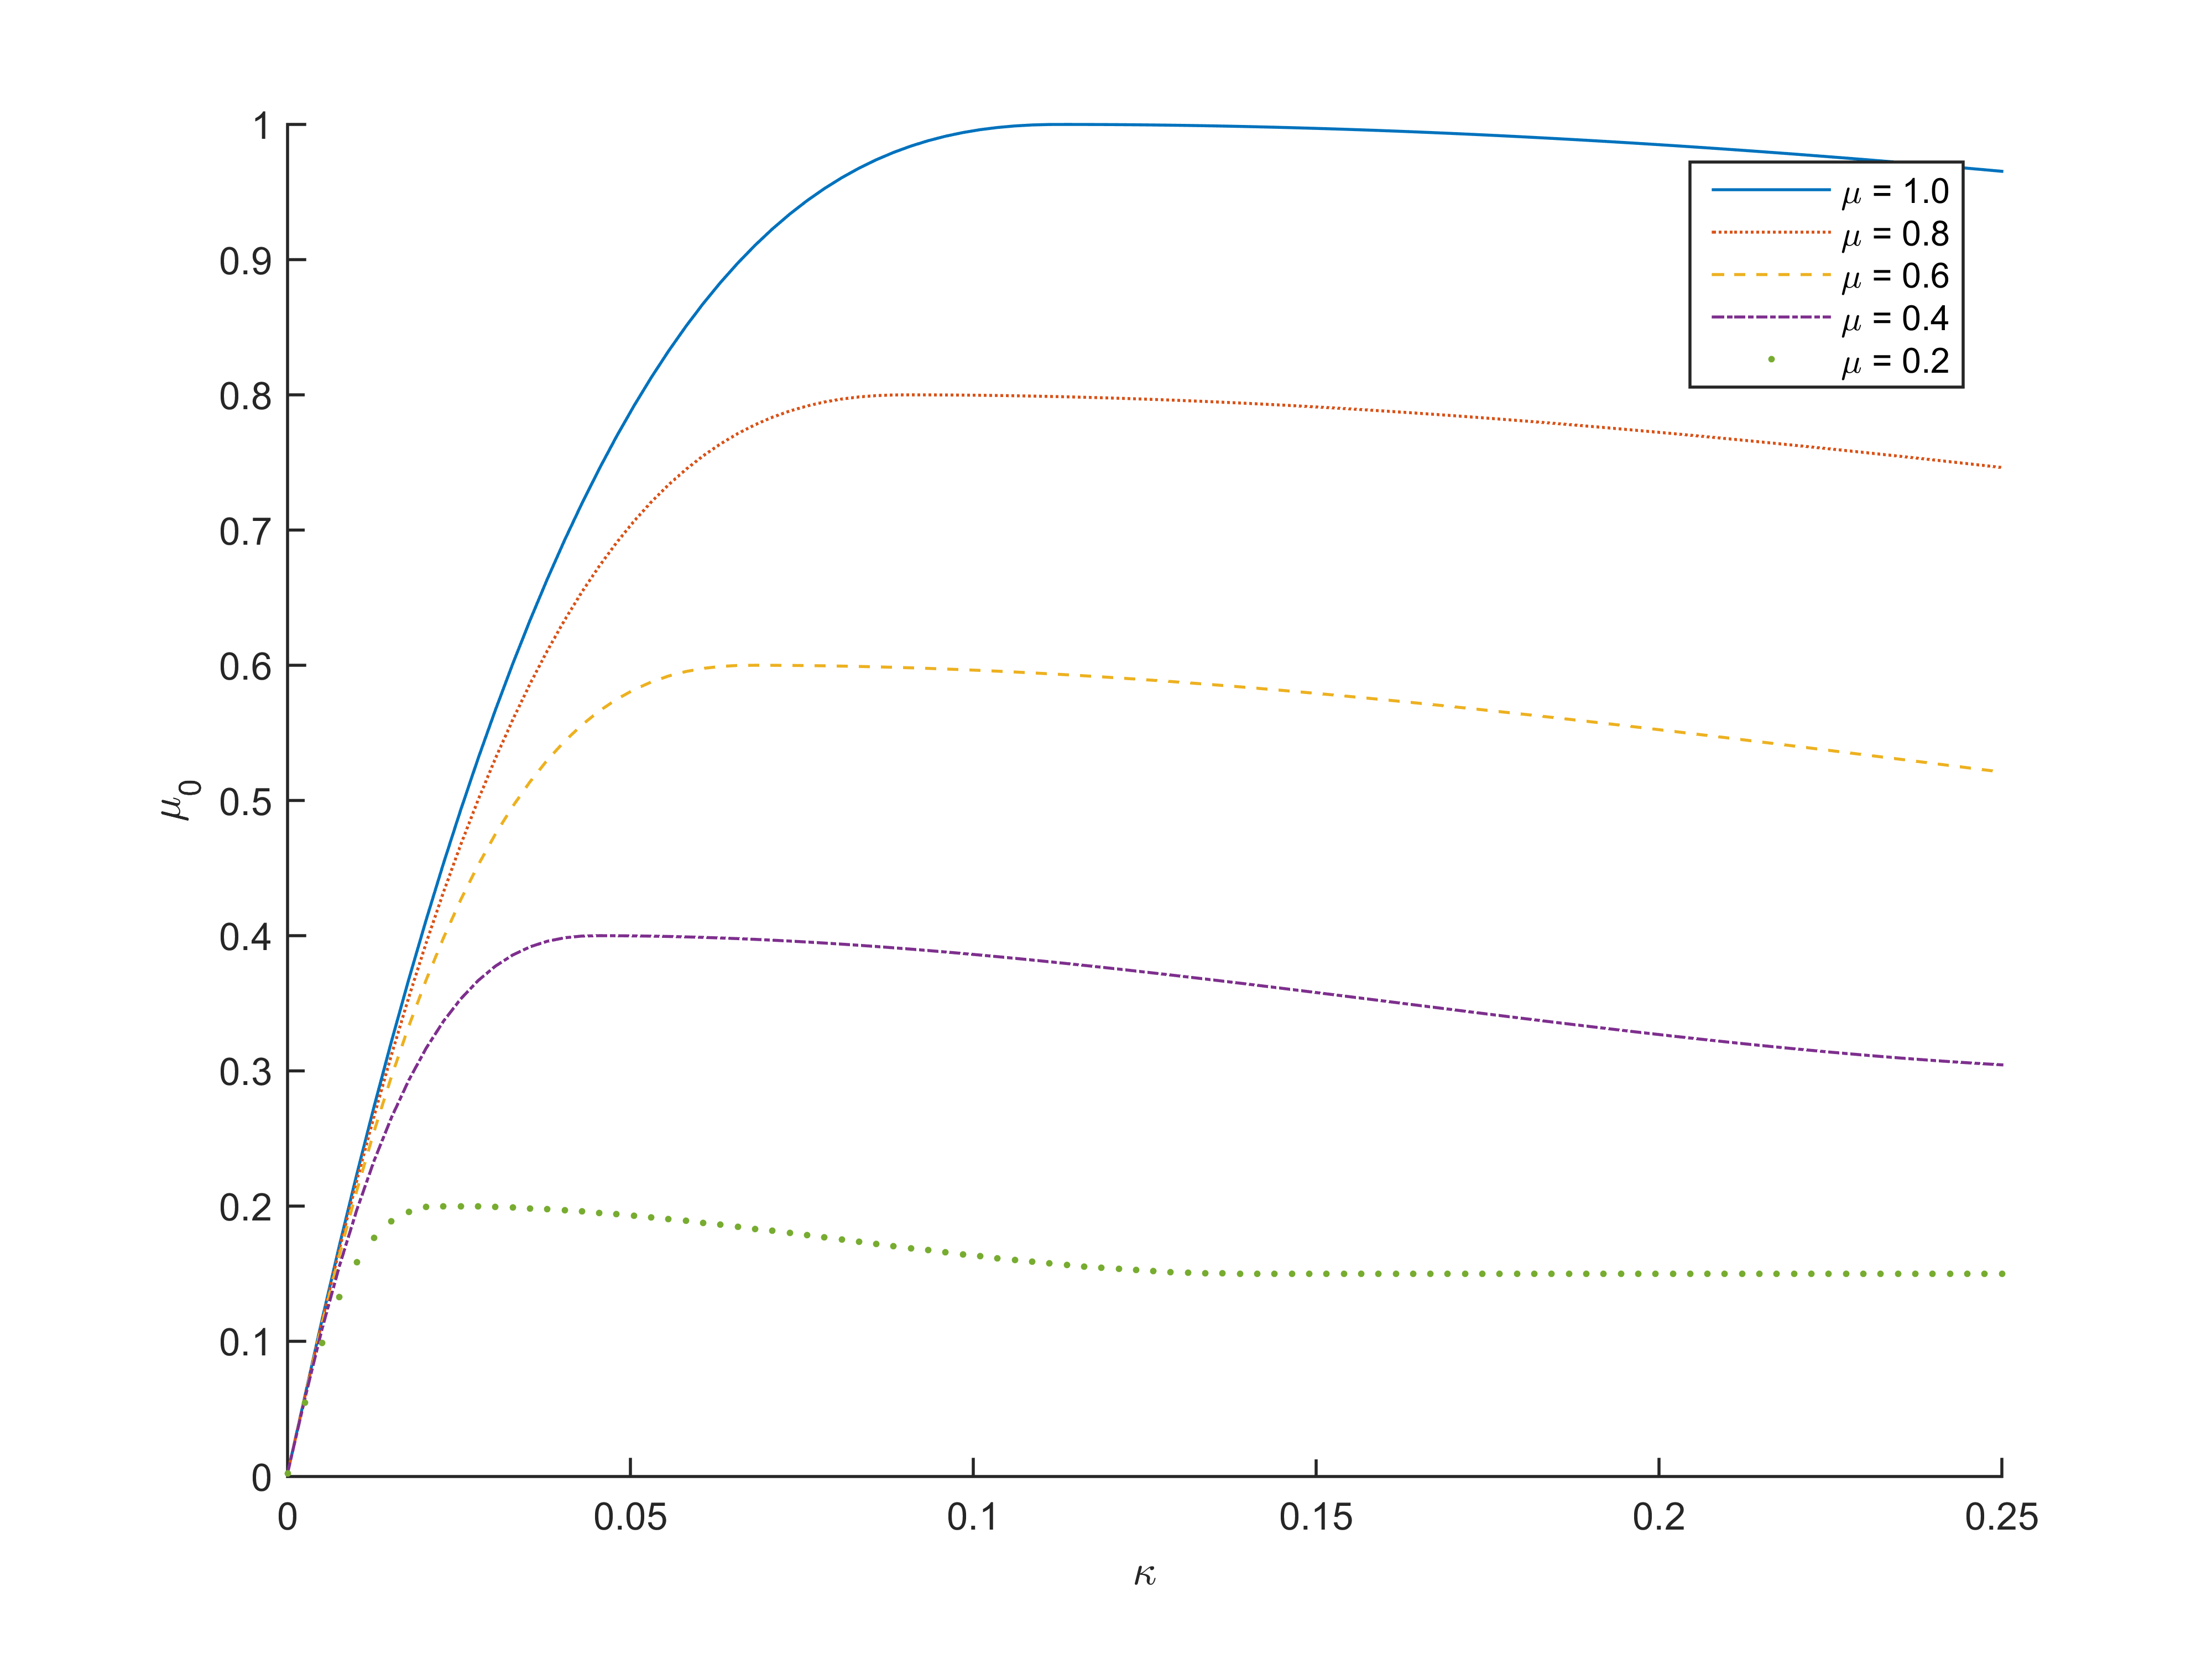
\includegraphics[width=1.0\textwidth]{Pictures/slipkraft_olika_mue}
	\caption {Normalized tire model force per slip ratio for different mue values.}
	\label{different_mue}
\end{figure}

\todo{add more}

\section{Fitting the tire model}
It is, as seen in the previous section (\ref{tire_forces}), very important to know the parameters that affect the force derived from the tire model. Slip ratio and the normal force is derived by using CAN signals from the vehicle and the friction coefficient is the parameter that should be approximated. The tire stiffness on the other hand is harder to approximate with good accuracy. The definition is, as mentioned earlier, the gradient of the slip/force curve around zero slip ratio, which means that the tire stiffness should preferably be approximated at small slip ratio values, where the gradient is relatively constant. The force per slip ratios between $ 0 $ and $ 2 $ can be seen in figure \ref{slip_kraft_sma_slip}. The figure shows that the variance of the force per slips ratio is rather large around the approximated line at $ C_{x} = 24 $. These tire stiffness variations for different driving scenarios makes it very hard to approximate the tire stiffness in a correct manner.

\begin{figure}[h]
	\centering                
	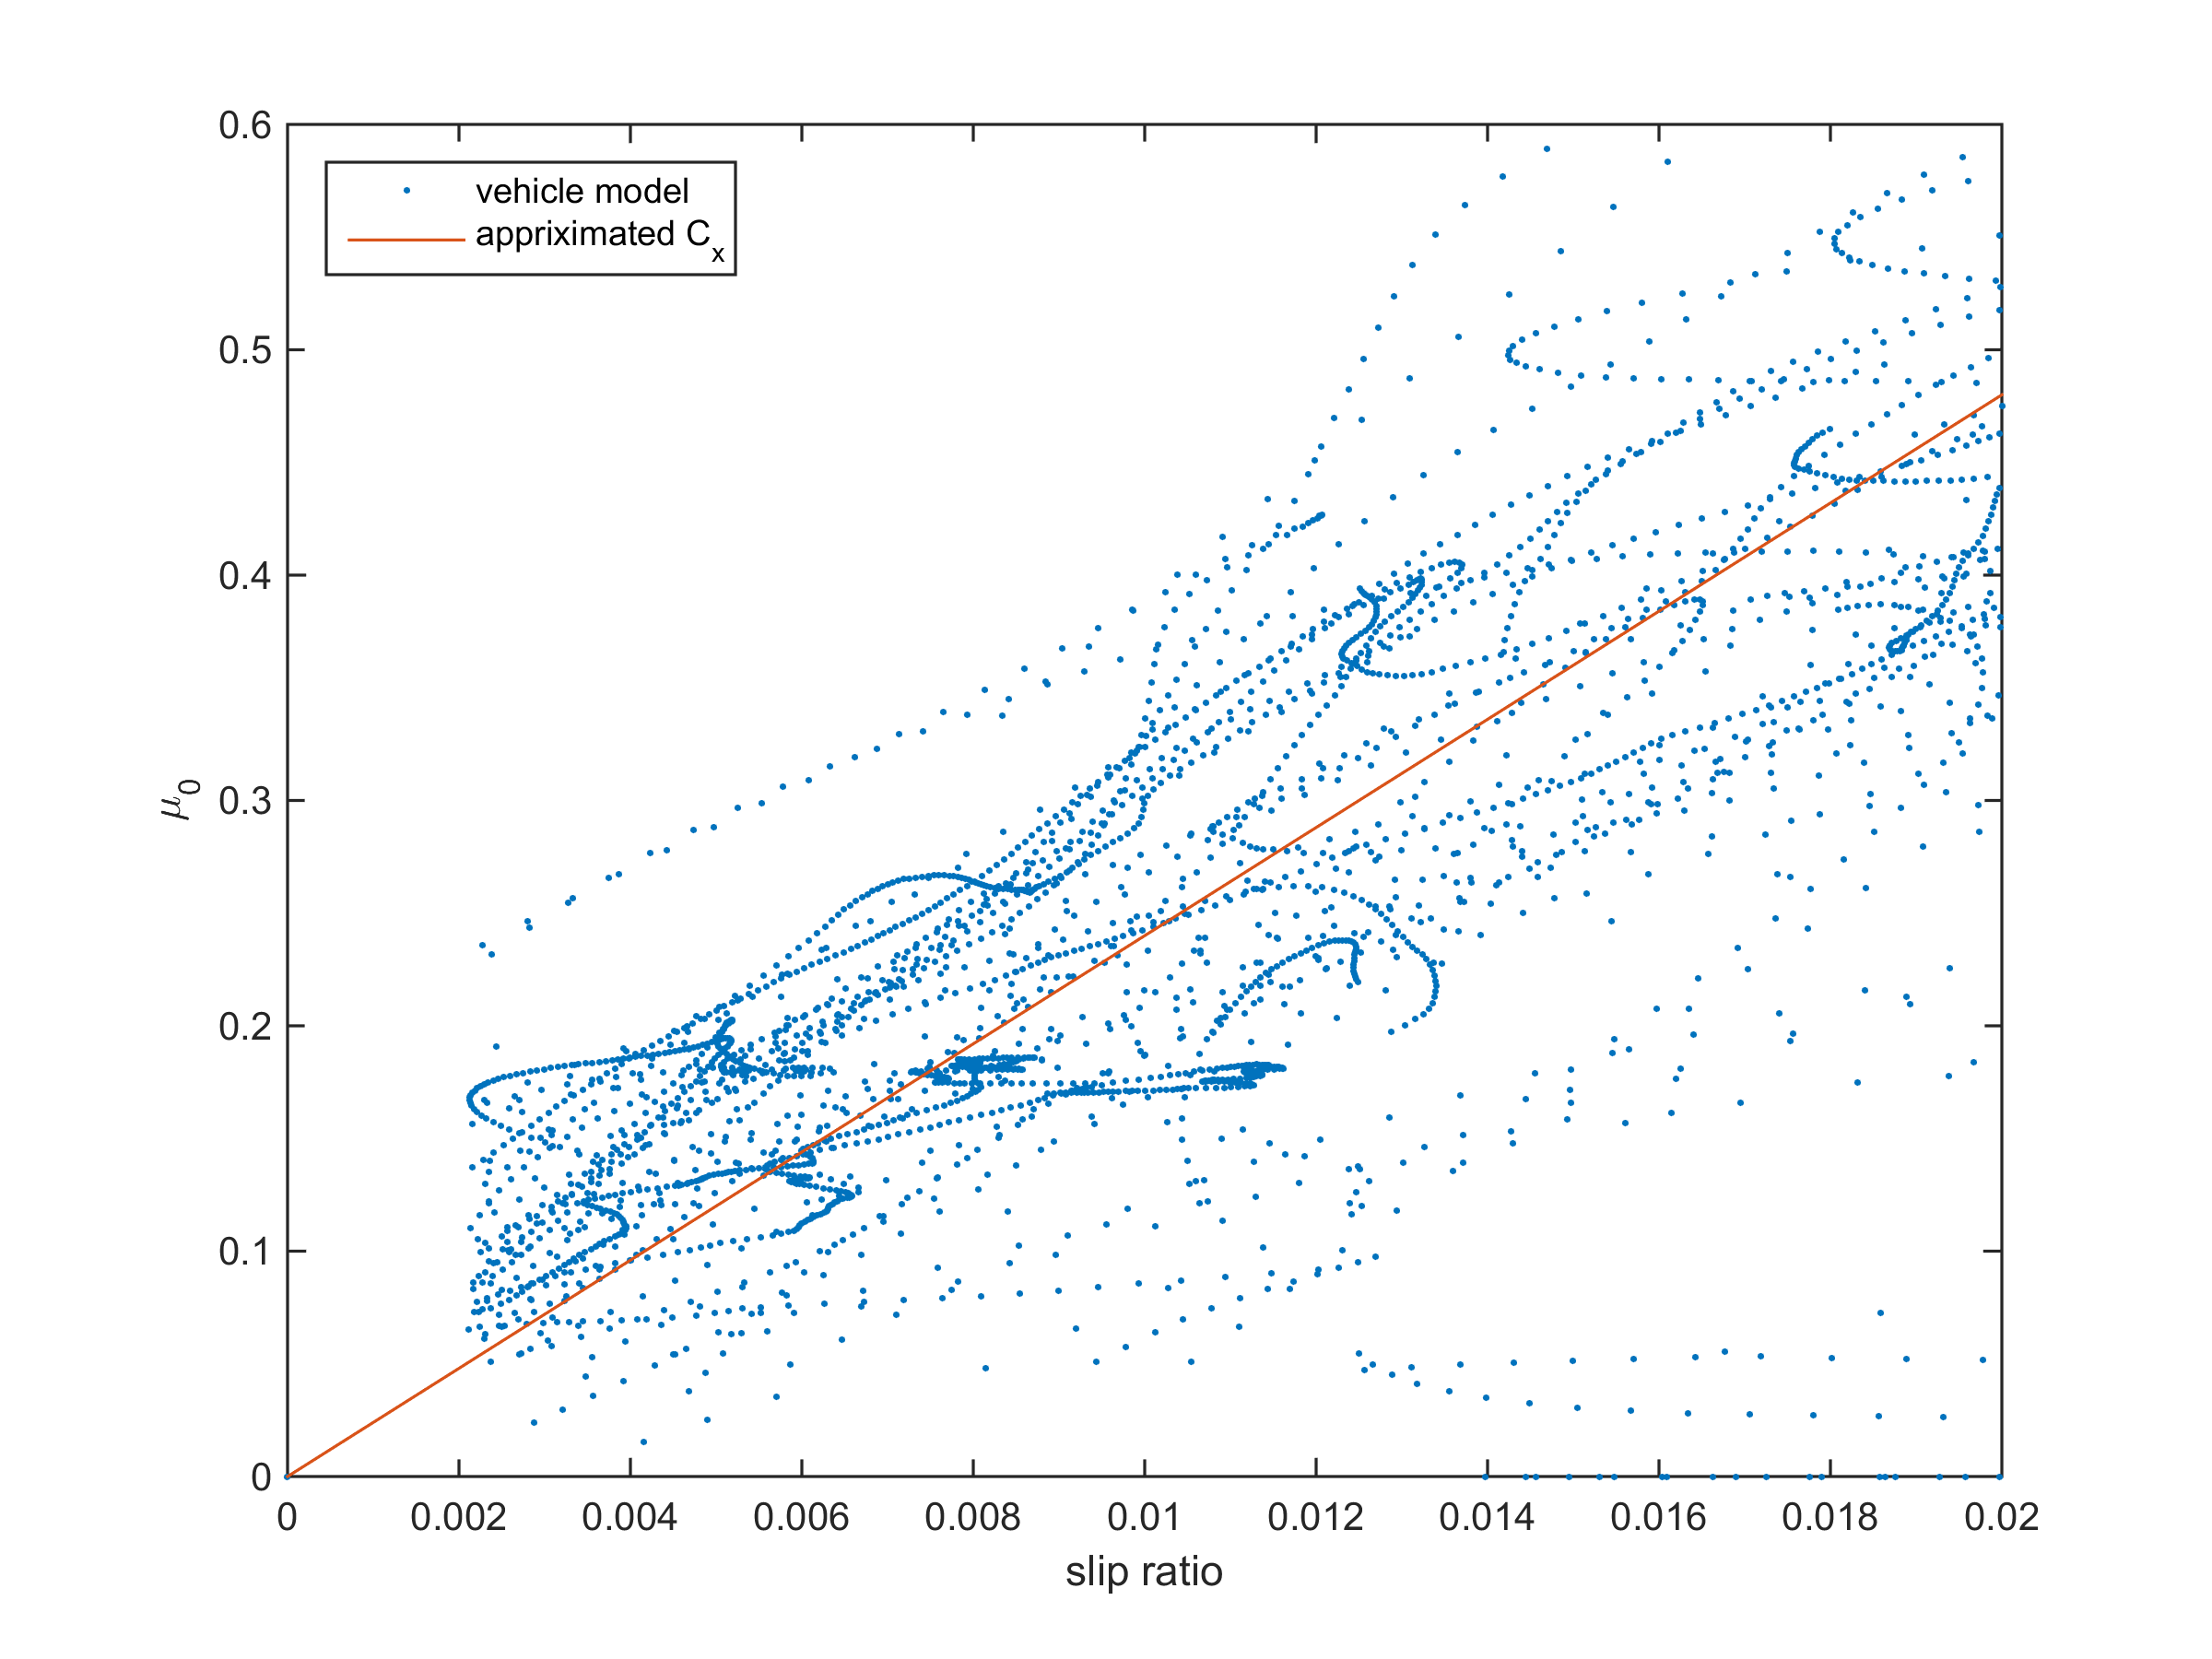
\includegraphics[width=0.8\textwidth]{Pictures/slip_kraft_sma_slip}
	\caption {Force per slip for lower slip ratio values can be used to estimate the tire stiffness.}
	\label{slip_kraft_sma_slip}
\end{figure}

Due to the difficulties to estimate the tire stiffness, experimentations has been made to fit tire model parameters during test driving. The problem with this solution is that static tire model parameters would be chosen for a certain driving sequence instead of having a dynamic solution that works for every kind of tire. 

It was also found during testing that the tire stiffness for the same set of tires changes depending on friction coefficient between the tire and the road. The tire stiffness will therefore be interpolated between two different tested tire stiffness values depending on the friction coefficient.

\subsection{Winter tires}
Test driving has been done with a set of winter tires on both asphalt and ice/snow. In figure \ref{slip_kraft_ljungby} the force per slip can be seen during a simple acceleration run on asphalt. It should be noted that only values for when the actual friction estimation is active is used. The tire model parameters that was fitted to the data and the friction coefficient became:
\begin{equation}
\label{winter_asphalt}
\begin{split}
	C_{x} = 24 \\
	\xi = 0.9 \\
	\mu = 1.0 \\
\end{split}
\end{equation}

\begin{figure}[h]
	\centering                
	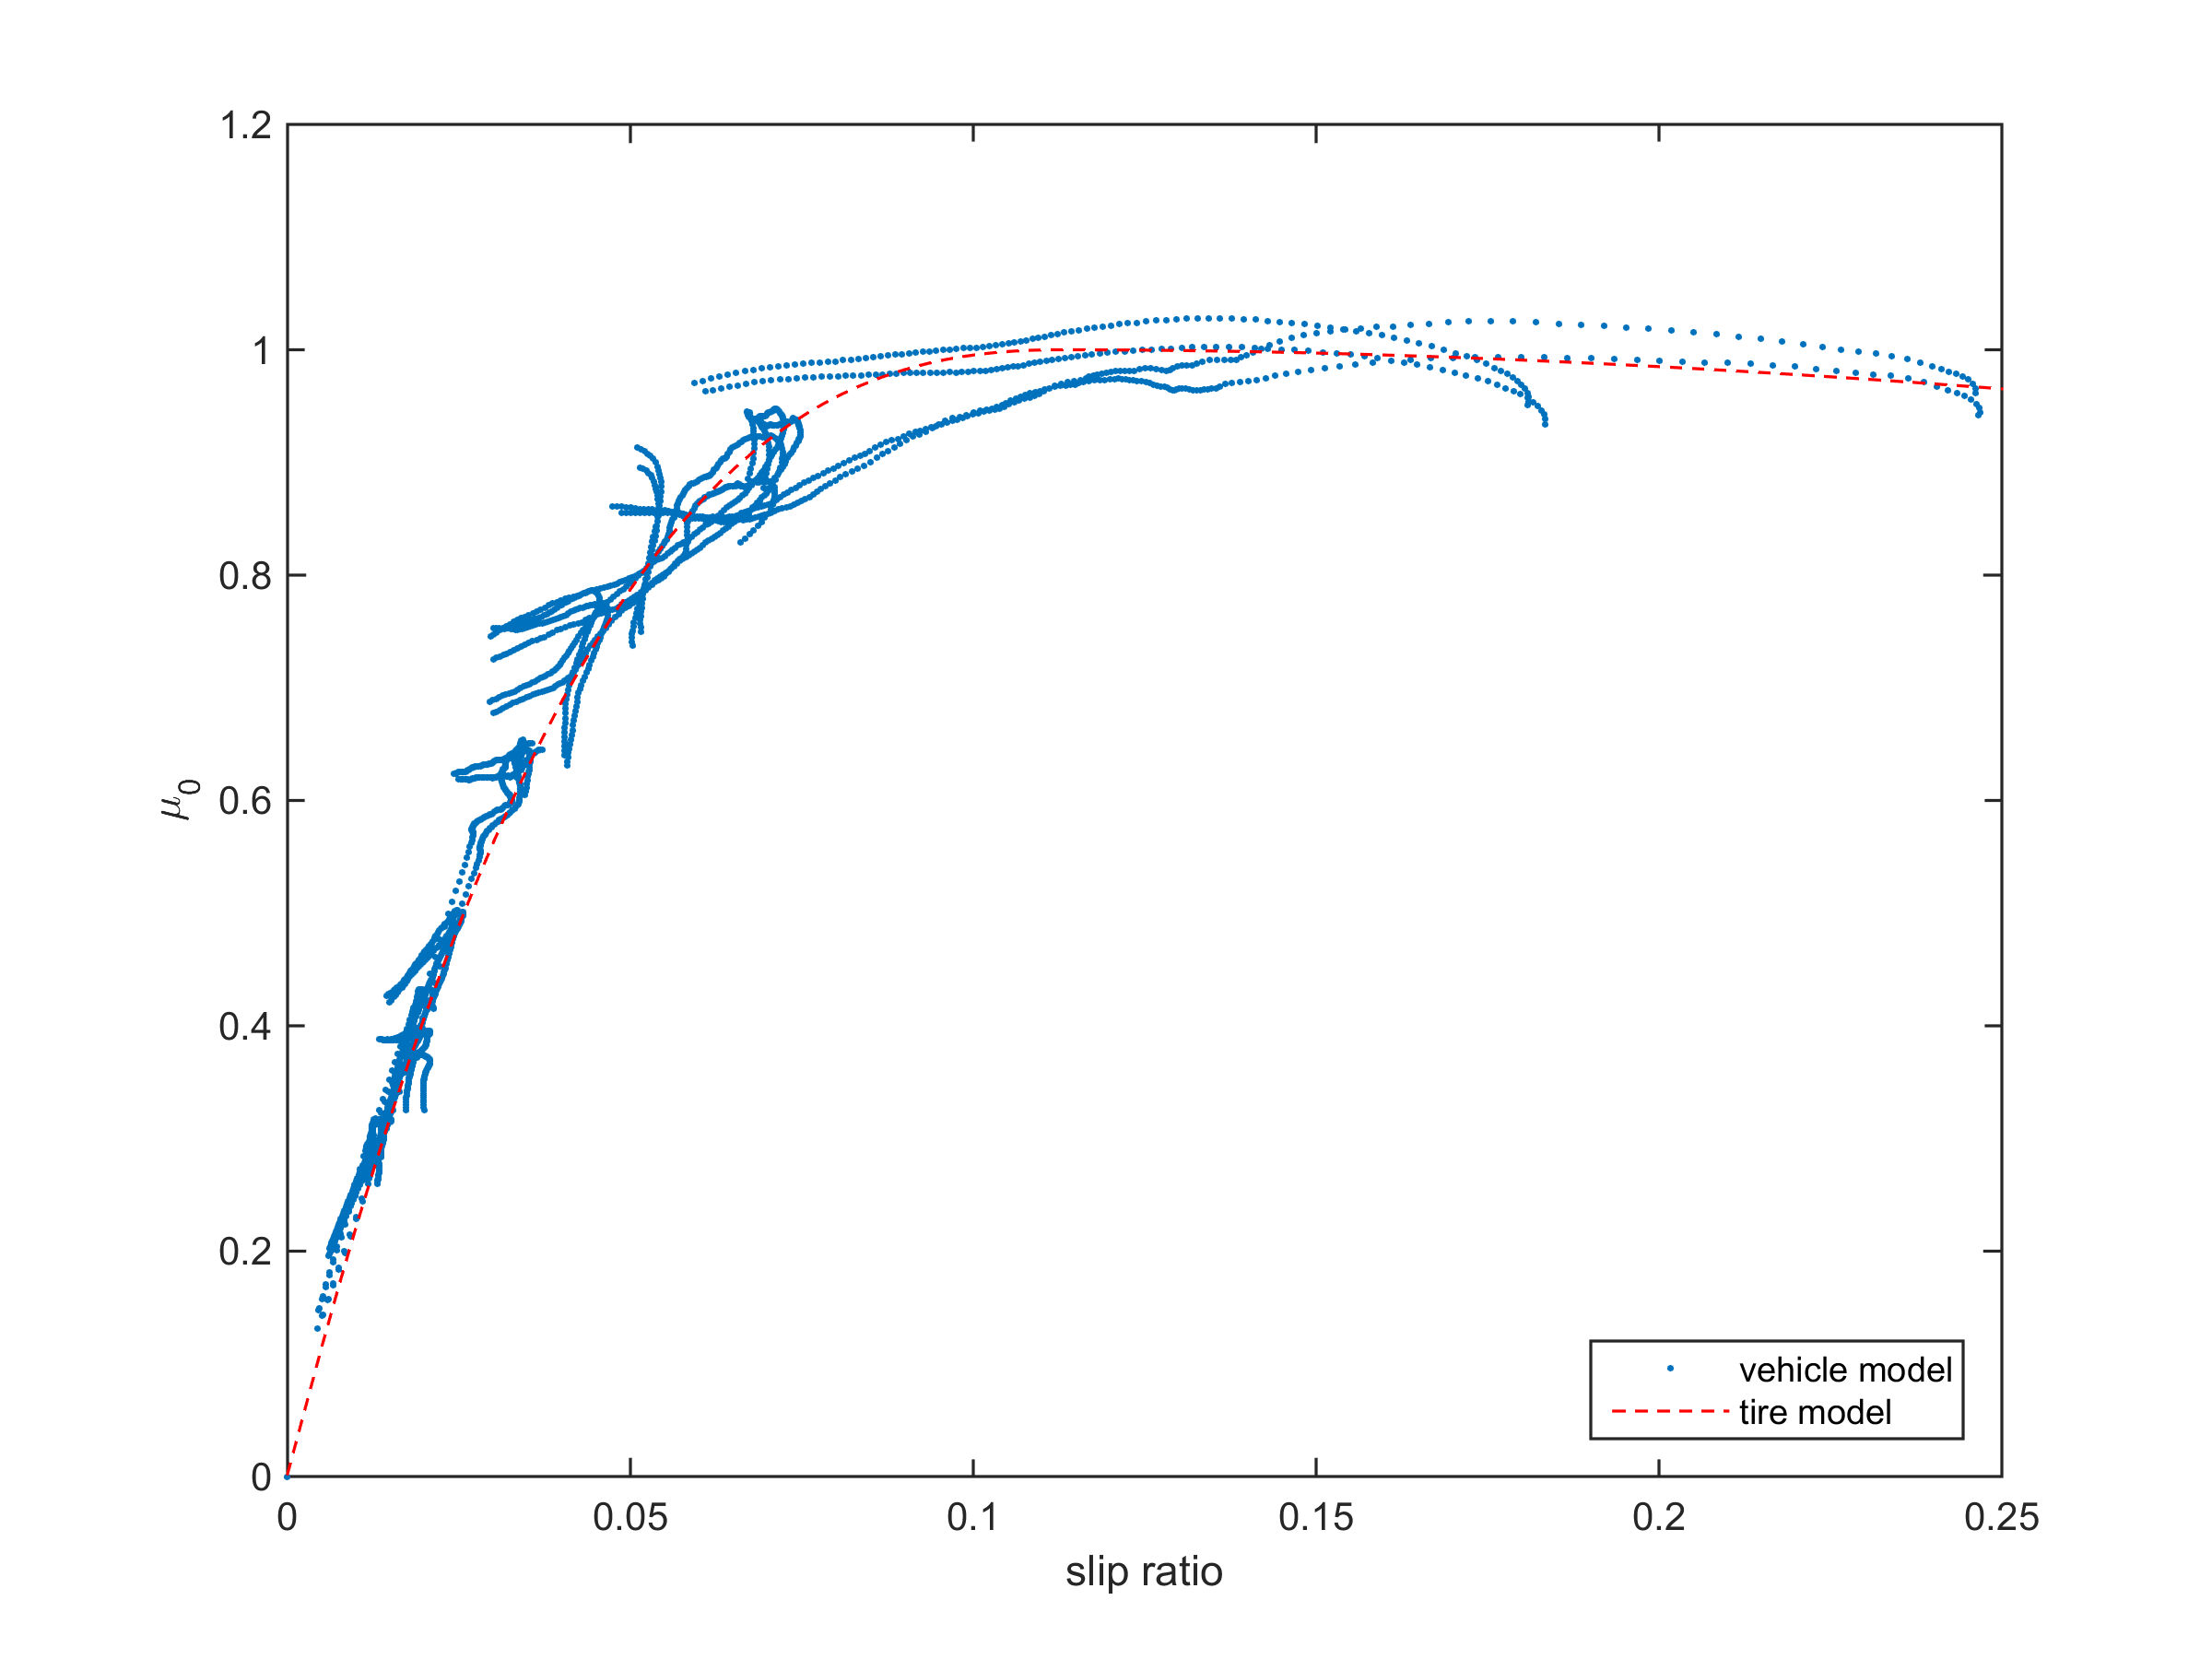
\includegraphics[width=0.8\textwidth]{Pictures/slip_kraft_ljungby}
	\caption {Normalized force per slip ratio for acceleration in a straight line with winter tires on asphalt.}
	\label{slip_kraft_ljungby}
\end{figure}

In figure \ref{slip_kraft_is} the force per slip can be seen during a driving sequence on ice/snow. This driving sequence was made on a track and not merely an acceleration in a straight line. The effect of this is more variance in the vehicle force calculation compared to the result in figure \ref{slip_kraft_ljungby}. The parameters for the fitted tire model and the friction coefficient for the ice driving sequence became:
\begin{equation}
\label{winter_ice}
\begin{split}
	C_{x} = 9.5 \\
	\xi = 0.9 \\
	\mu = 0.4 \\
\end{split}
\end{equation}

\begin{figure}[h]
	\centering                
	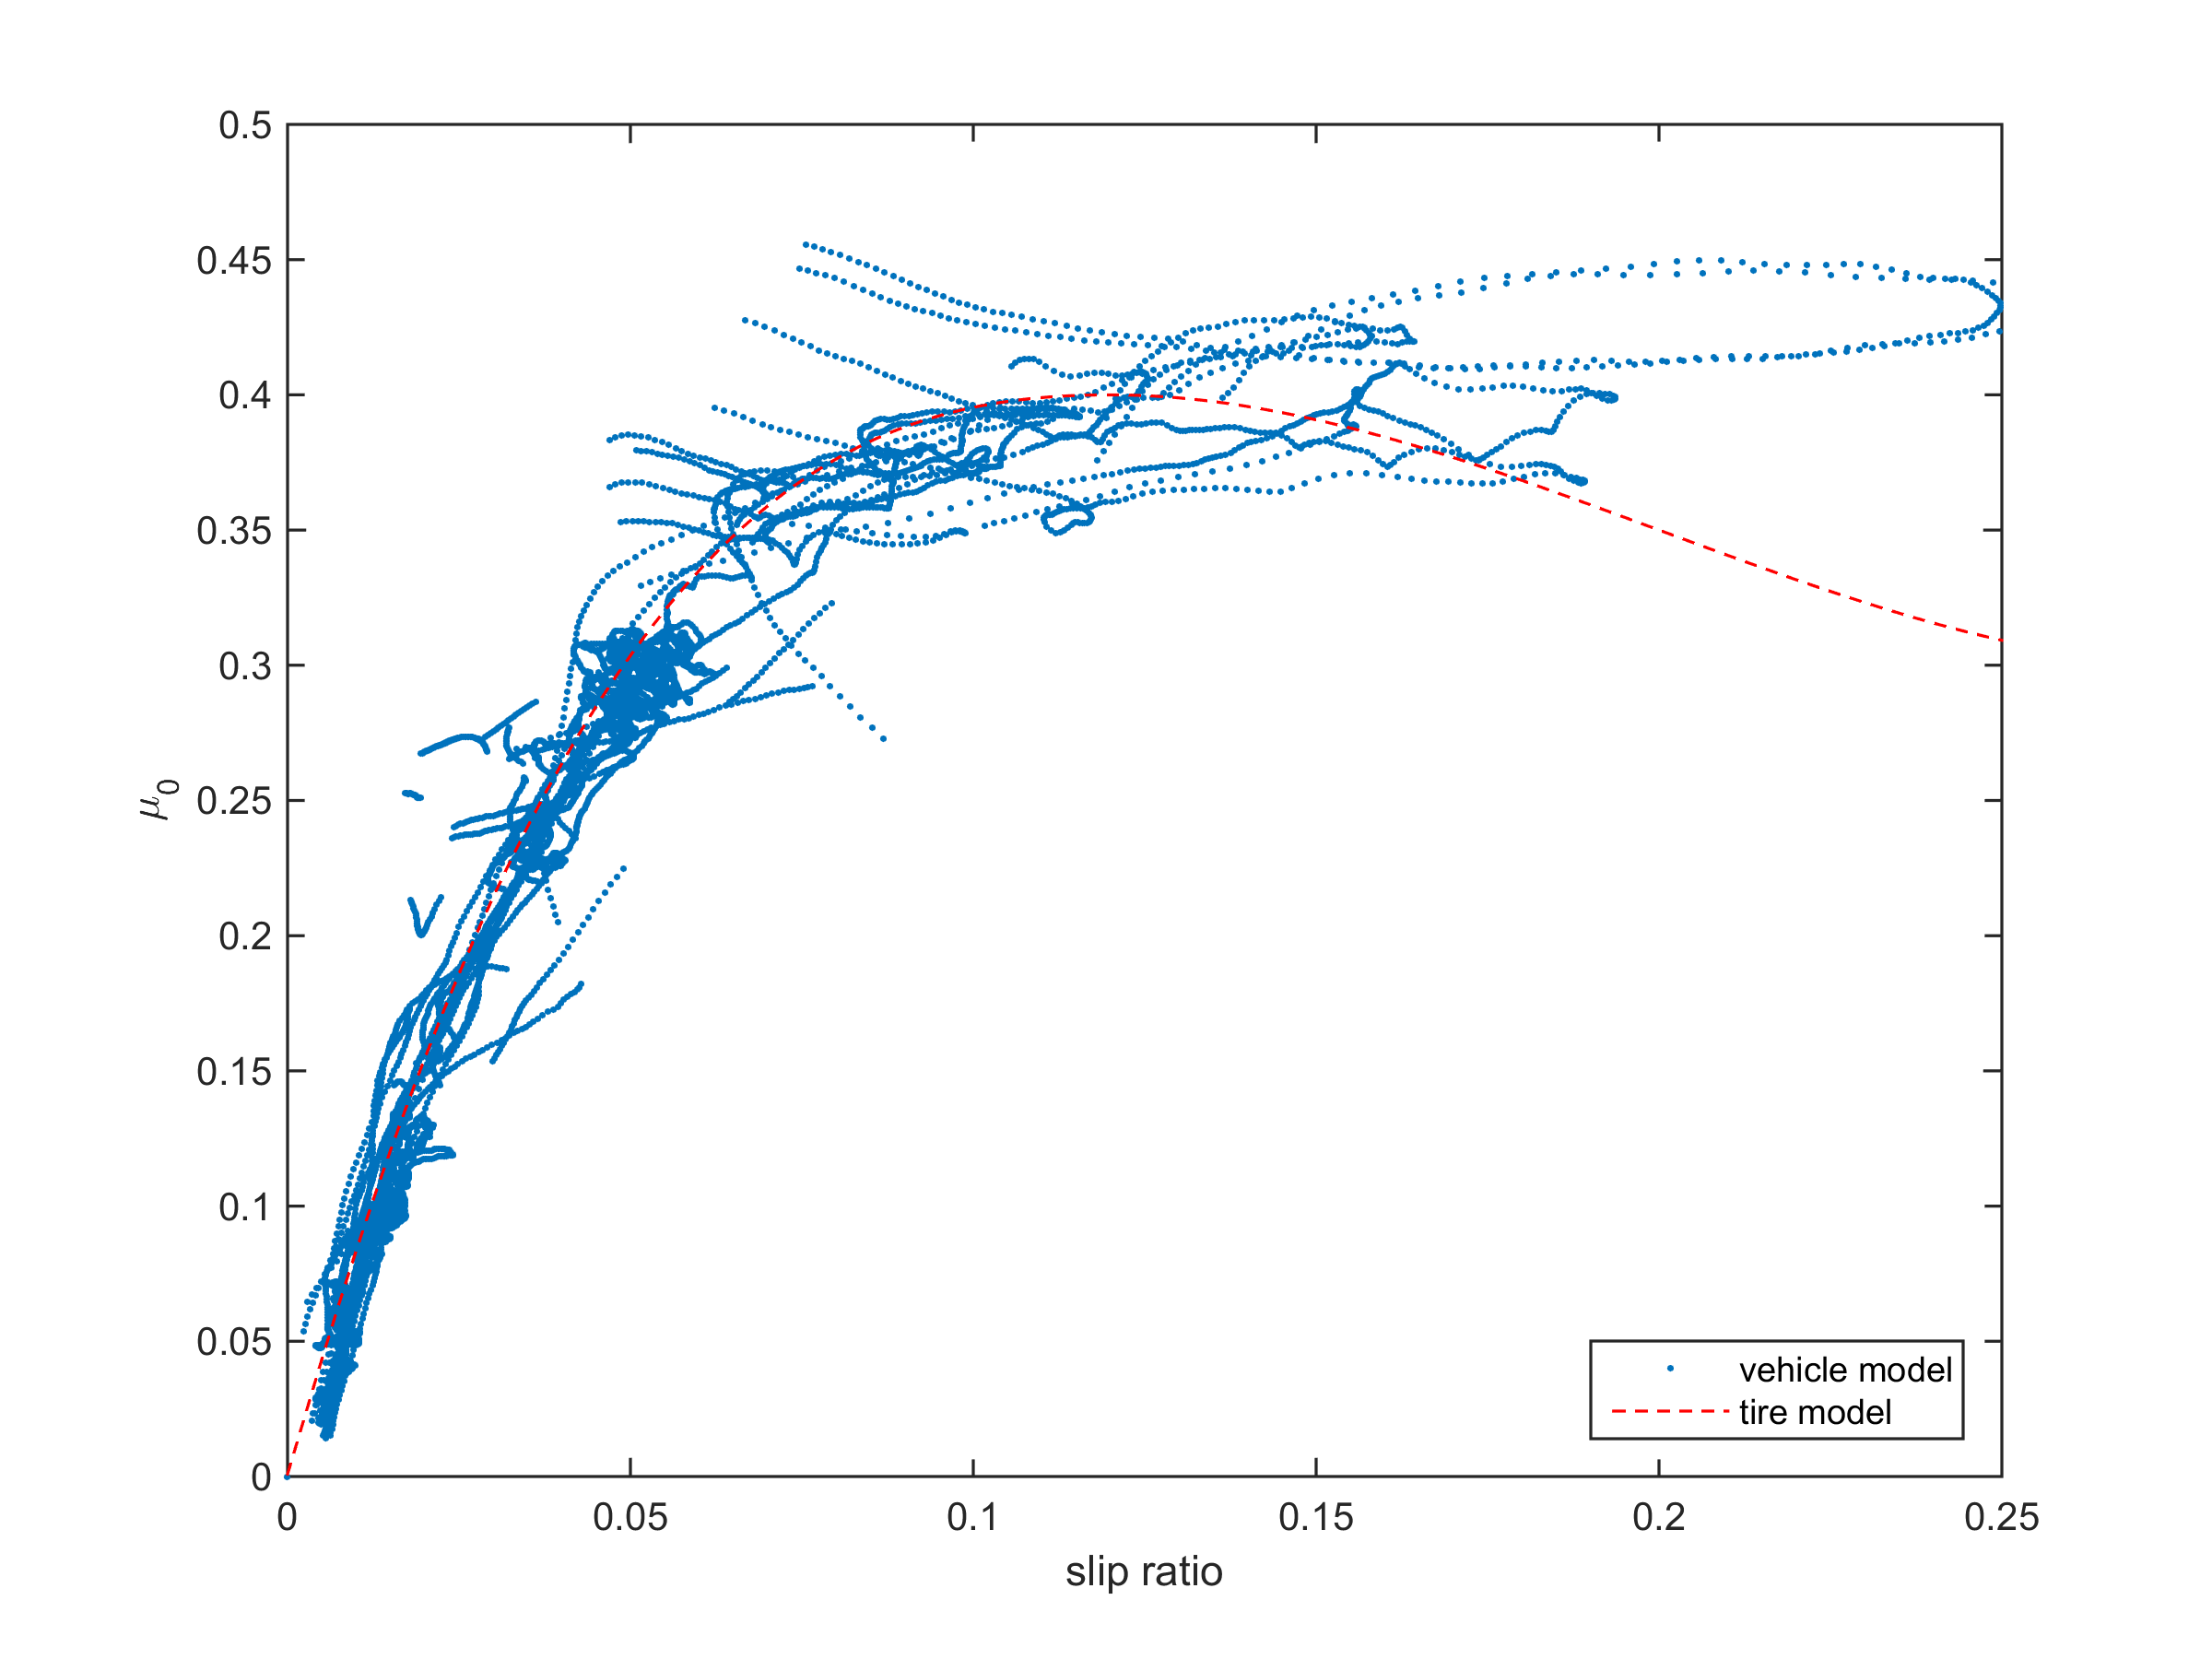
\includegraphics[width=0.8\textwidth]{Pictures/slip_kraft_is}
	\caption {Normalized force per slip ratio for a track run on ice/snow with winter tires.}
	\label{slip_kraft_is}
\end{figure}

To get the correct tire stiffness for different friction coefficient, a straight line was fitted between $ C_{x} $ and $ \mu $ in \ref{winter_asphalt} and \ref{winter_ice}. This first degree fitting results in:
\begin{equation}
	C_{x} = 25\mu - 1
\end{equation}

\subsection{Summer tires}
Test driving has also been made with a set of summer tires on asphalt. The tires used were low profile tires which generally means high stiffness, i.e. low slip ratio values are needed to acquire the same longitudinal force, which can be seen in figure \ref{slip_kraft_bb_torr}. The data acquired from this driving sequence does not include any slips above the force peak. Assuming that blah blah blah blah!
\begin{figure}[h]
	\centering                
	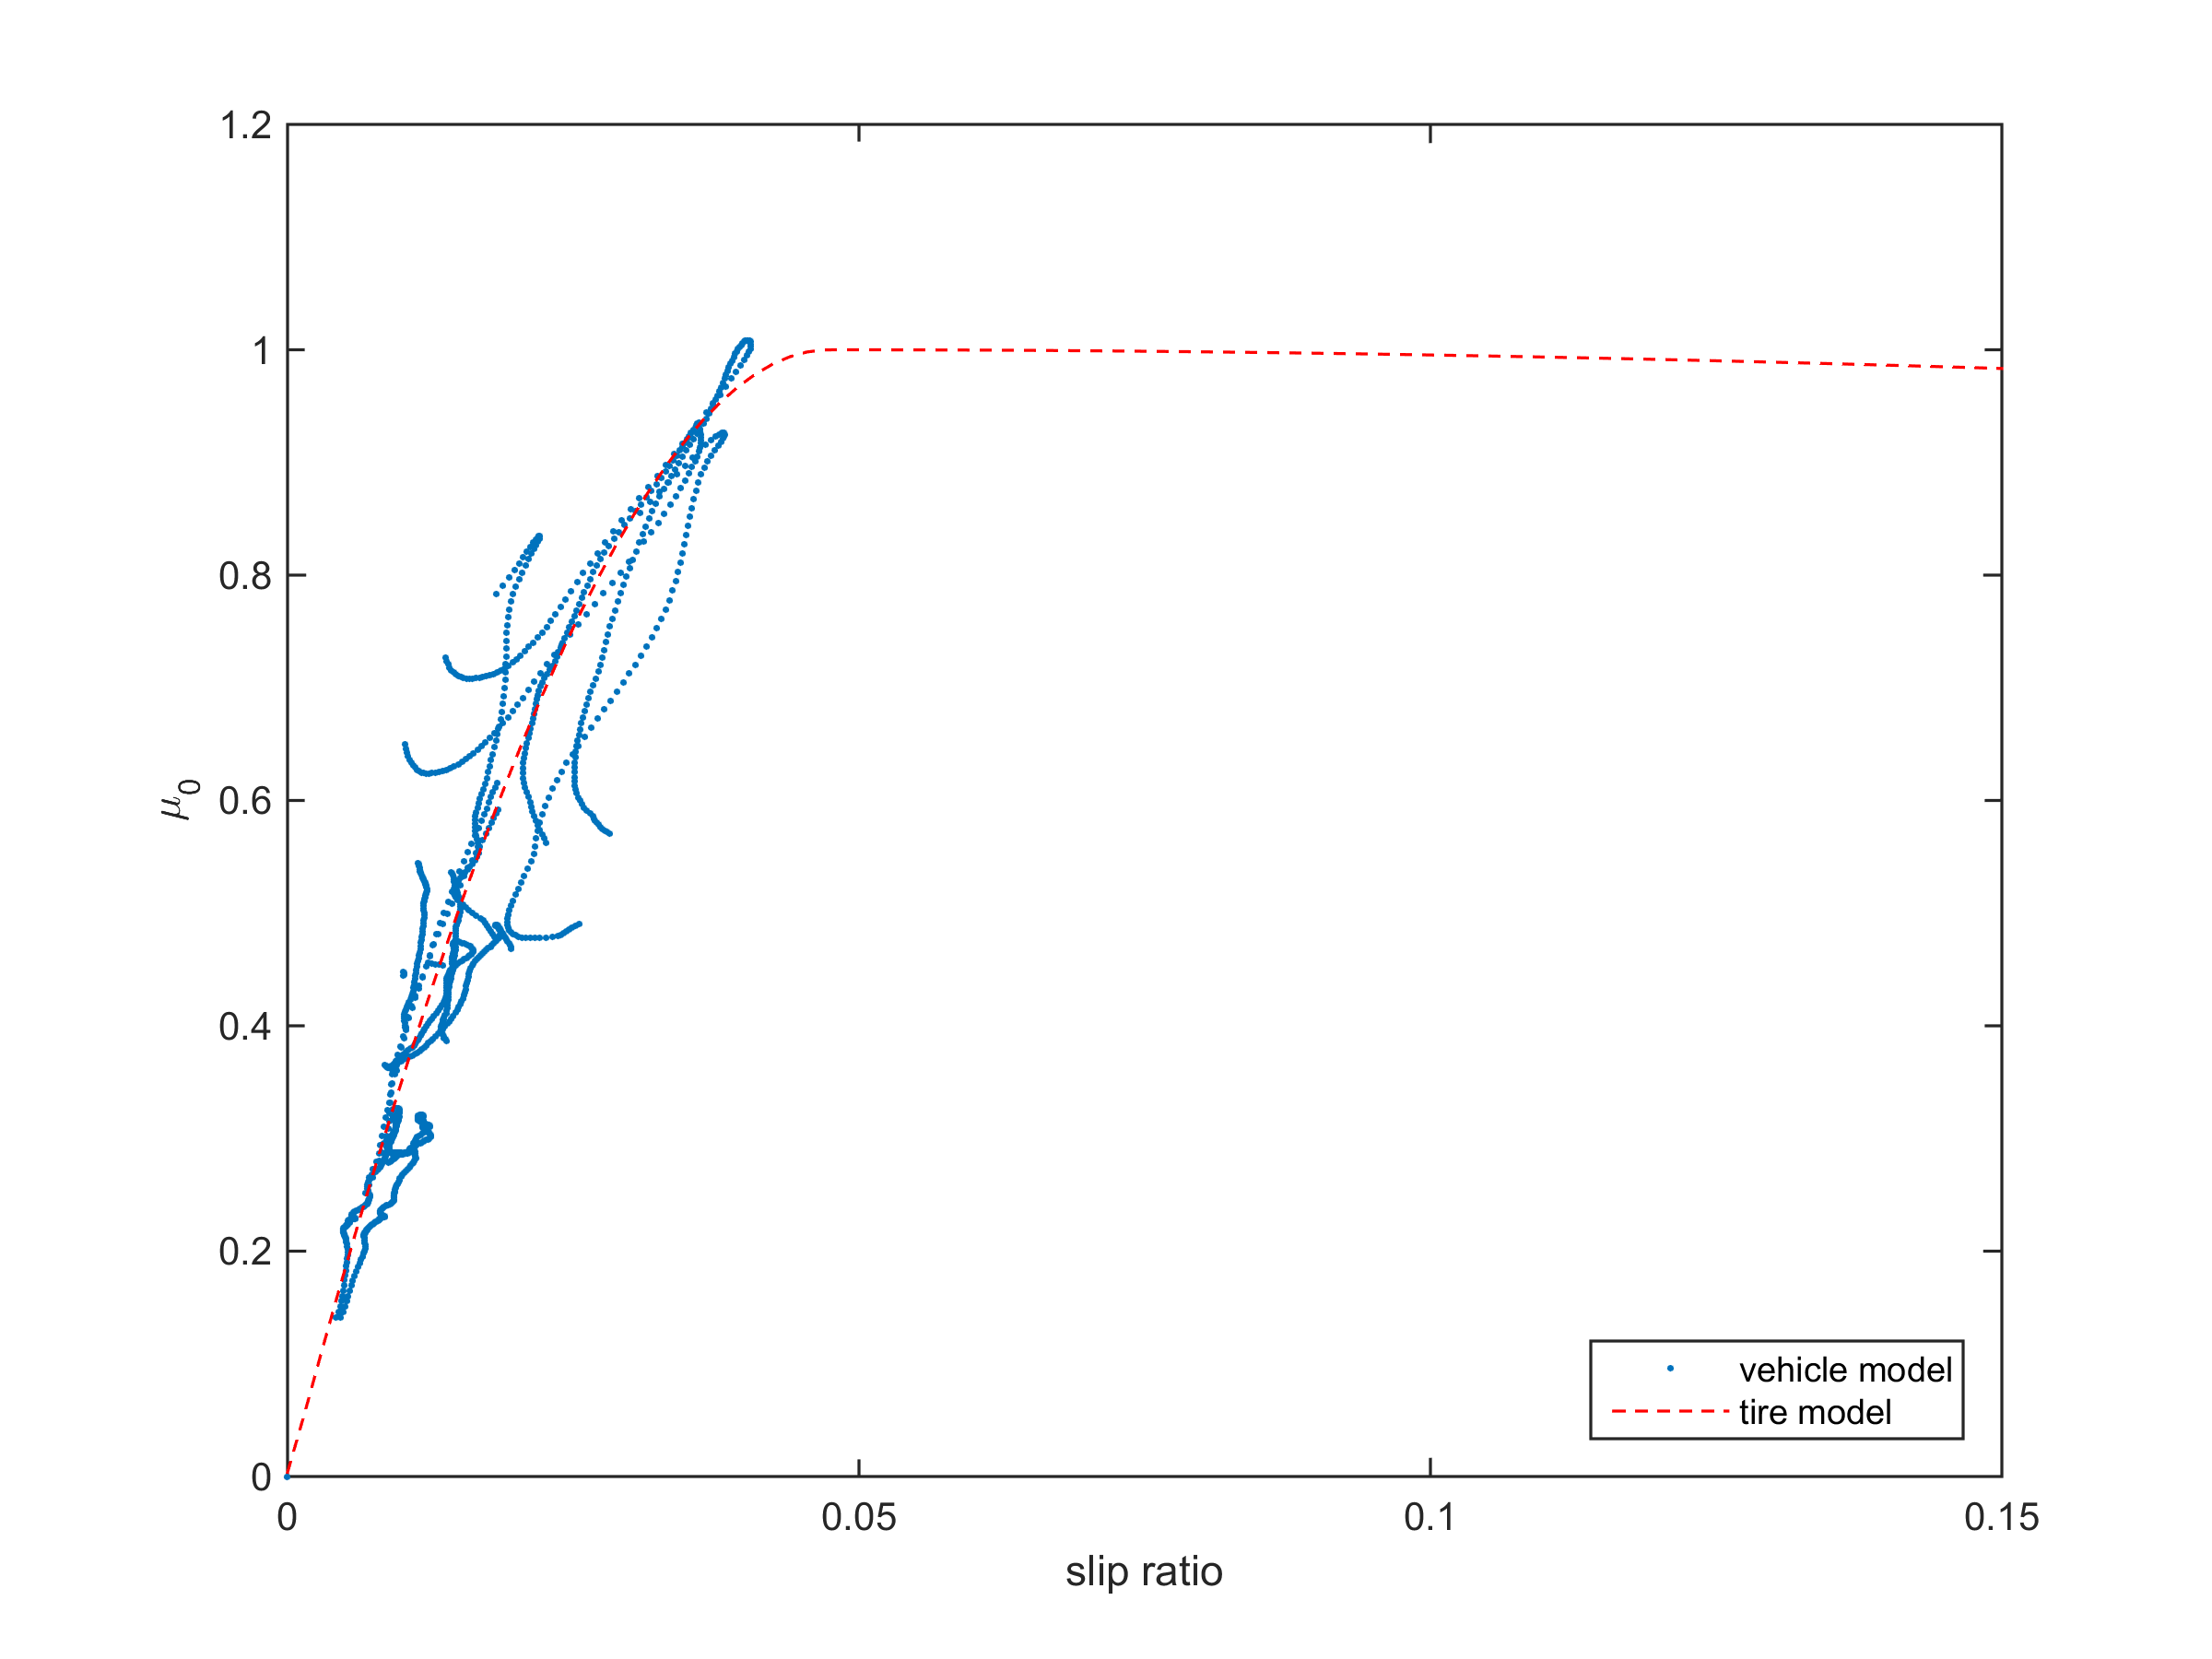
\includegraphics[width=0.8\textwidth]{Pictures/slip_kraft_bb_torr}
	\caption {Normalized force per slip ratio for acceleration in a straight line with summer tires on asphalt.}
	\label{slip_kraft_bb_torr}
\end{figure}

\subsection{Lateral acceleration compensation}
The force per slip curves seen in \ref{slip_kraft_ljungby} and \ref{slip_kraft_bb_torr}, where the tire model parameters are fitted, are derived from data acquired from merely accelerations done on a straight line. This means that no lateral forces are acting on the tires, which is very ideal conditions and unlikely during real driving sequences. When a vehicle is turning, it will also have a slip angle between the tires heading and pointing direction. When slip angle is present, the amount of longitudinal force actually generated per slip ratio will becomes less, see the curves for different slip angles in \ref{combined}. However, slip angle is a parameter which is hard to approximate, and assumed to be unknown in this report. A parameter that is correlated to slip angle is the lateral acceleration., which means that it is most likely that lateral acceleration is present when a slip angle is. 
 
An approximation for the new slip ratio that is to be used is derived by:
\begin{equation}
\label{slip_ratio_compensation}
\kappa_{a_{y} compensated} = \dfrac{\kappa}{1 + a_{y}\cdot \beta}
\end{equation}
Where $ \beta $ represent how much the lateral acceleration should be considered. In Figure \ref{latacc_compensated}, two different force per slip ratio curves can be seen for a driving sequence which include cornering at high speeds, meaning that slip angle as well as lateral acceleration is present. The data is taken from a driving sequence using the same winter tires as seen in Figure \ref{slip_kraft_ljungby}, and therefore also using its fitted tire model parameters from Equation \ref{winter_asphalt}. In the first subplot of Figure \ref{latacc_compensated}, no compensation for lateral acceleration is considered, while the data in the second subplot uses the new approximated slip ratio derived by Equation \ref{slip_ratio_compensation} using $ \beta = 0.15 $. 
\begin{figure}[h]
	\centering
	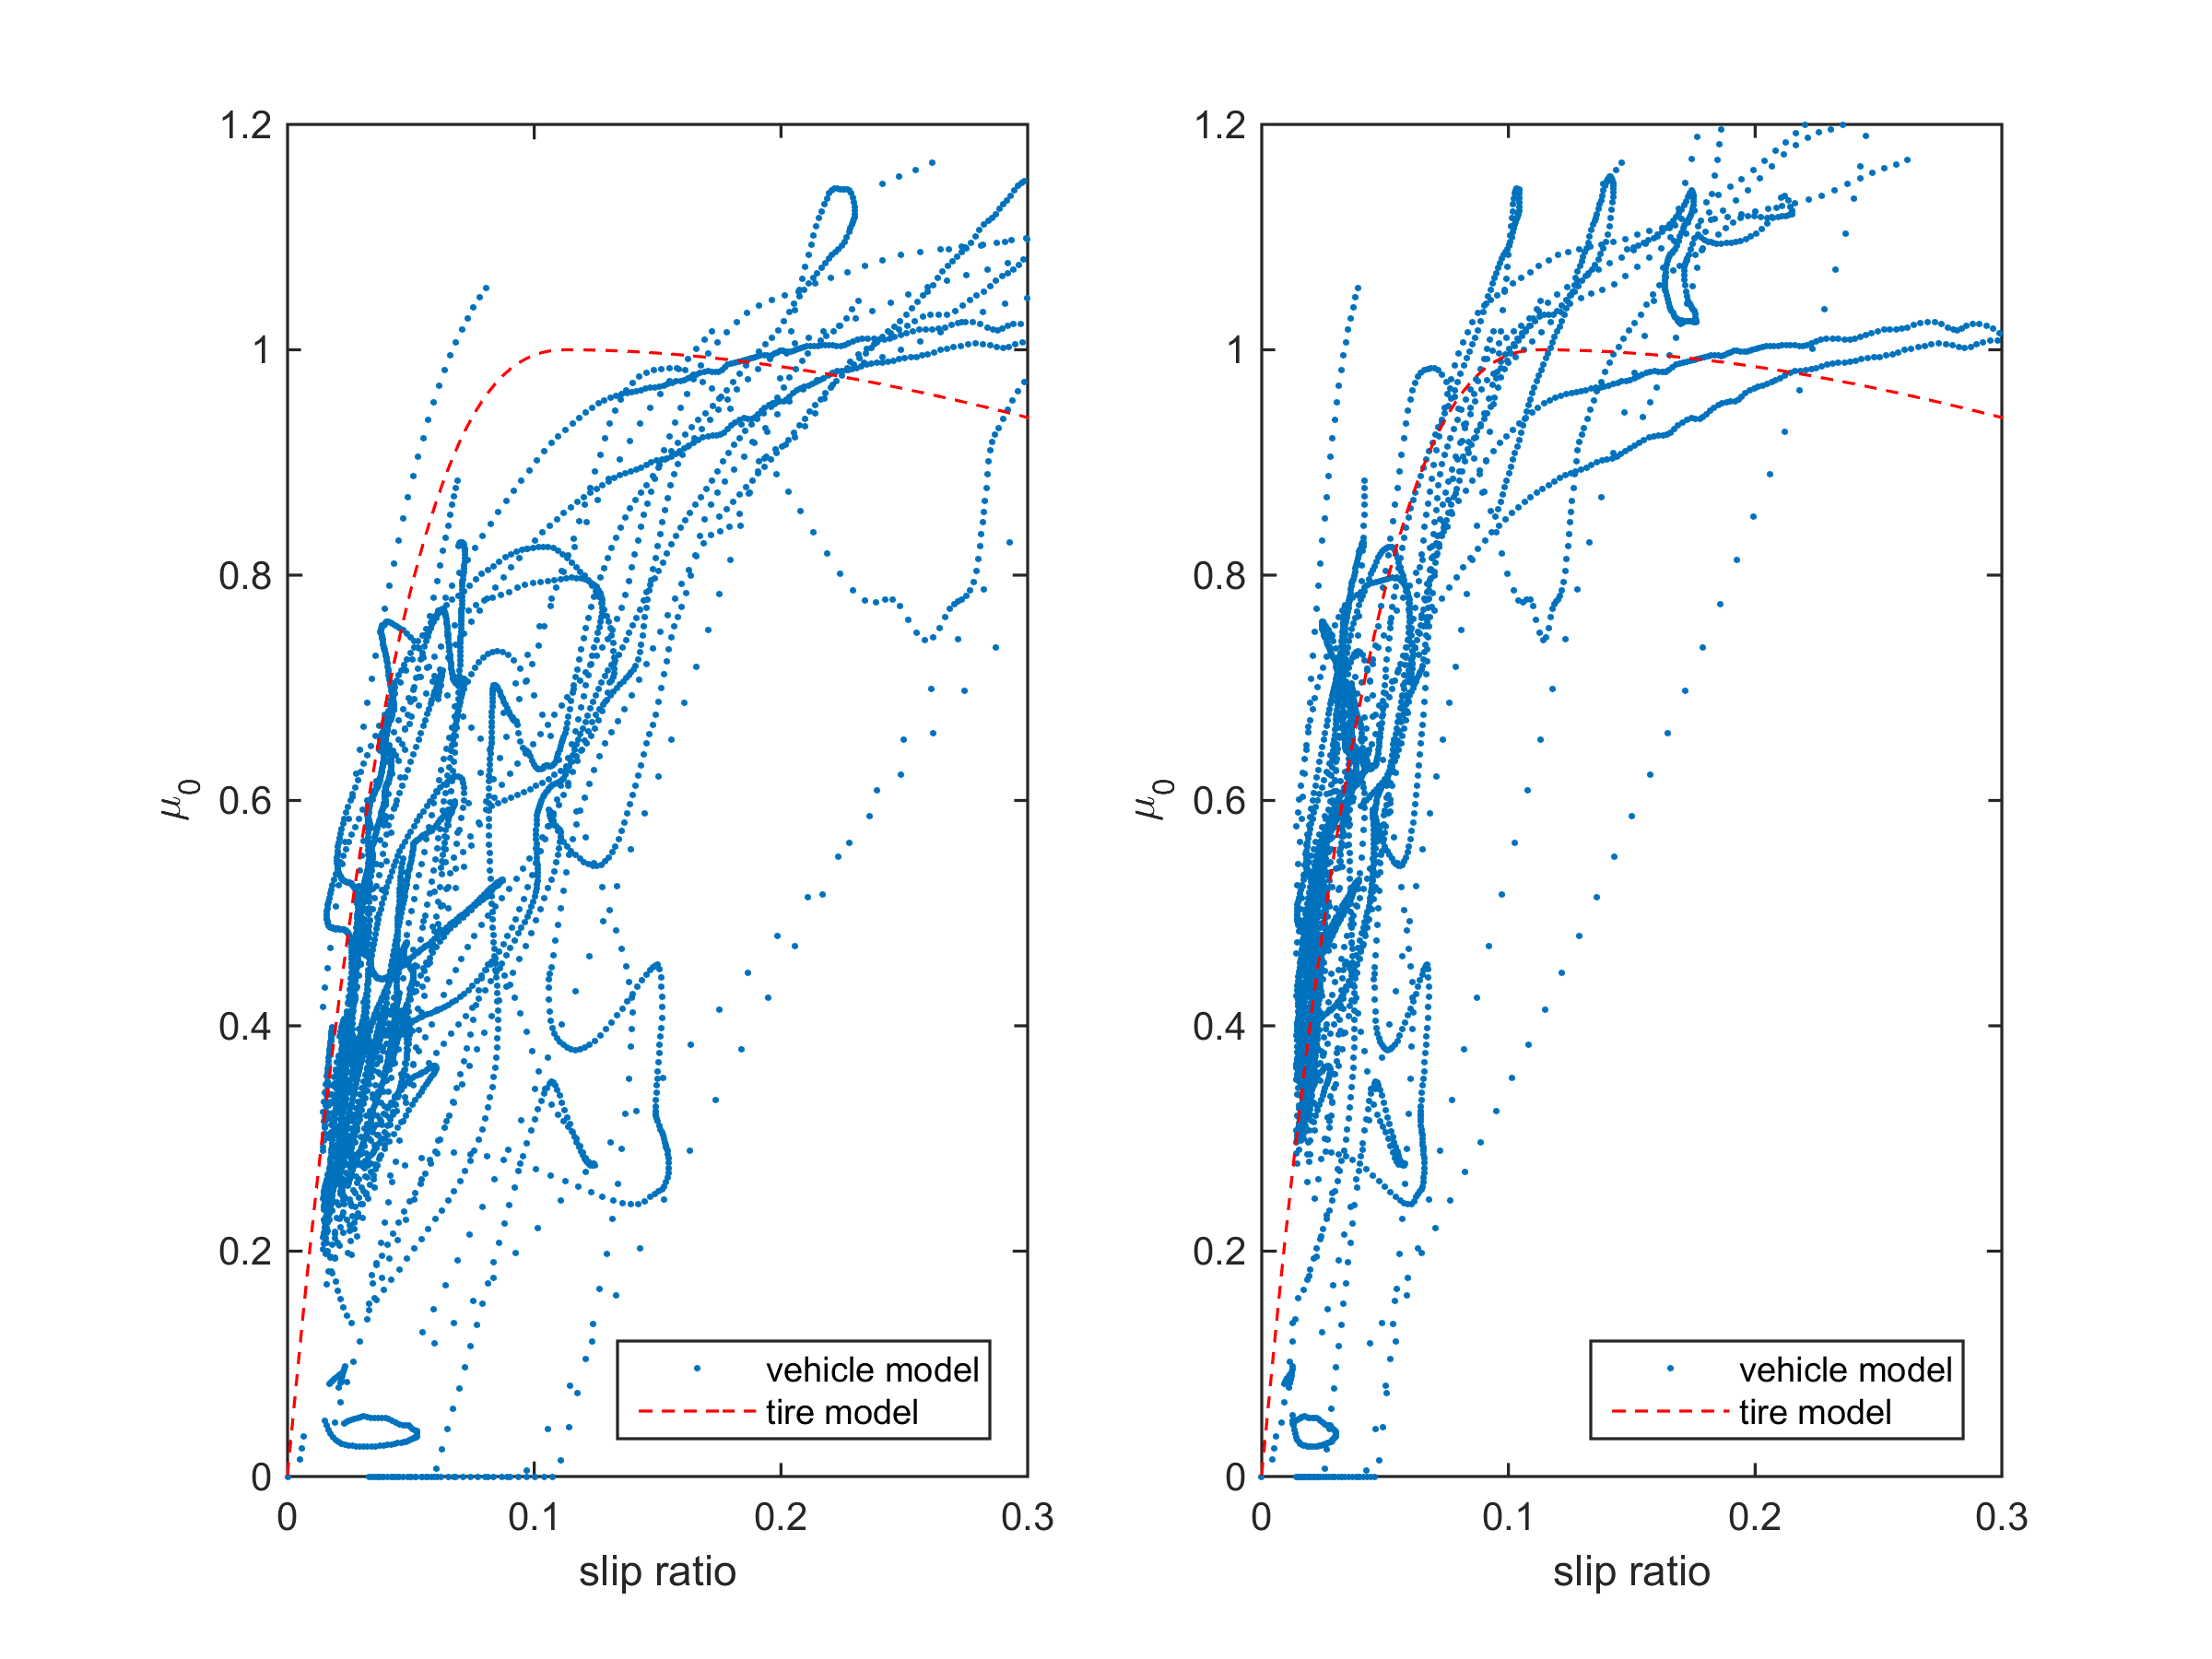
\includegraphics[width=1.0\textwidth]{Pictures/latacc_compensated}
	\caption {Normalized force per slip ratio when slip ratio is compensated due to lateral acceleration.}
	\label{latacc_compensated}
\end{figure}

\section{Estimating the friction coefficient}
The aim om the friction estimation is, as mentioned earlier, to choose the correct friction coefficient so that the forces from the two different models become alike. In other worlds, choose the $ \mu $ that enables:
\begin{equation}
	F_{vehicle} = F_{tire}
\end{equation}
This relation, and therefore also a friction coefficient, could theoretically be obtained at every instance when new CAN packages are available. This would lead to a rapid changing friction coefficient which wouldn't reflect the actual tire/road friction. Instead of approximating a new friction coefficient at every moment, a least square fitting method is used to find the friction coefficient. The goal of such a method is to find the friction coefficient that provides the smallest error between the two models over a certain amount of time. 

\subsection{Least square fitting}
The general idea of a least square fitting method is to minimize the sum of the squares between a theoretical model and observed data. 
\begin{equation} 
	y(k) = \phi(k)\cdot\theta + v
	\label{eq:least_square}
\end{equation}
Where $ y $ is the observed data, $ \phi(k)\cdot\theta $ the theoretical model and $ v $ the error. The cost function that should be minimized becomes the following:
\begin{equation}
	V(\hat{\theta}, k) = \dfrac{1}{2} \sum_{i=1}^{k} \lambda^{k-i}\Big(y(i) - \phi(i)\cdot\hat\theta \Big)^2
\end{equation}
Due to the fact that new data is acquired continuously, these least square approximations would need to be executed at every time step, creating unreasonable amount of computations. Hence, a modification of the least square fitting is used which recursively takes previous results into account.

\subsection{Recursive least square fitting}
The recursive least square (RLS) fitting method is defined as:
\begin{equation}
	L(k) =\dfrac{ P(k-1)\phi (k)}{\lambda + \phi (k) P(k-1)\phi(k)} 
\label{eq:RLS1}
\end{equation}
\begin{equation}
	P(k) = \Big( 1 - L(k)\phi (k) \Big) \dfrac{1}{\lambda} P(k-1)
\label{eq:RLS2}
\end{equation}
\begin{equation}
\hat \theta (k) = \hat \theta (k-1) + L(k) \cdot v(k)
\label{eq:RLS3}
\end{equation}
Where the error is:
\begin{equation}
	v(k) = y(k) - \phi (k) \hat \theta (k-1)
	\label{eq:RLS4}
\end{equation}
L and P define how much the next $ \theta $ update should rely on the error. A larger L takes the error into account more, while a smaller number makes the update rely on the old $ \theta $ value more. The forgetting factor, $ \lambda $, is defined by the user and basically describes how many previous values to consider when calculating a new $ \theta $.

However, this method can only be applied to linear system, and a tire force, $F=f(\kappa, Fz, \mu, C_{x})$, is not linear. To able to use the RLS, the function has to be linearized. To accomplish this, the derivative of the force as a function of $ \mu $ is defined as:
\begin{equation}
	\dfrac{\partial F}{\partial \mu} = \dfrac{\partial f(\kappa, Fz, \mu, C_{x})}{\partial \mu}
\end{equation}
Which describes how much the force will increase dependent on $ \mu $. The force in that linearized region thereafter becomes:
\begin{equation}
	F_{vehicle} = \dfrac{\partial F_{tire}}{\partial \mu} \cdot \mu
\end{equation}
This function now has the same form as \ref{eq:least_square}, which means that the RLS method in \ref{eq:RLS1}-\ref{eq:RLS4} can be used. The RLS with its proper parameters is:
\begin{equation}
	L(k) =\dfrac{ P(k-1) \dfrac{\partial F_{tire}(k)}{\partial \mu}}{\lambda + \dfrac{\partial F_{tire}(k)}{\partial \mu} P(k-1) \dfrac{\partial F_{tire}(k)}{\partial \mu}} 
\end{equation}
\begin{equation}
	P(k) = \Bigg( 1 - L(k) \dfrac{\partial F_{tire}(k)}{\partial \mu} \Bigg) \dfrac{1}{\lambda} P(k-1)
\end{equation}
\begin{equation}
	\mu (k) = \mu (k-1) + L(k) \Big( F_{vehicle} (k) - F_{tire} (k) \Big)
\end{equation}
The friction coefficient value is updated every step and depends on its own value, the error between the vehicle and tire model, and the number L describing how much to rely on the error. $ \dfrac{\partial F_{tire}}{\partial \mu} $ becomes larger for slips close to the peak force, which means that larger changes of $ \mu $ is possible at that point. The forgetting factor, $ \lambda $, is usually a value in the region $ [0.9, 1) $, where a larger forgetting factor means that older values are considered more, resulting in slower changes of $ \mu $.

\subsection{When to estimate the friction coefficient}
In a perfect world, it would be desired to be able to estimate the friction coefficient during every driving situation in order to capture any sudden change of grip between the tire and the road that can be present. Unfortunately there exist many challenges during most driving sequences that have to be considered. During some situations, either the vehicle or the tire model are shown to capture the occurrence far from its reality. These situations need to be identified so that the RLS fitting method does not update the estimated friction coefficient value at these period of times. This means that the friction coefficient value will no be continuously updated throughout every driving sequence and that sudden changes of the tire/road friction can be missed.

\subsubsection{Limitations due to slip ratio }
There are a couple of driving sequences that affect the slip ratio in such a way that the forces cannot be modeled correctly. When braking, the slip ratio should be close to zero assuming braking forces on all tires, meaning that tire forces cannot be modeled. During cornering, the front wheels will be turned creating a lateral force and a yaw rate. The rear, which doesn't have any positive cornering effect, will follow the front wheels but in a smaller radius, leading to a lower velocity. This difference in velocity between the front and rear wheels will result in a slip ratio that is non proportional to the amount of force generated at the tires. This phenomena will be larger when cornering at low speeds, due to the fact that a smaller lateral force is acting, and therefore not pushing the rear axle to a larger radius. This large slip ratio due to cornering can be seen in figure \ref{turning_slow_Vx}. At around $ 20 $ s and after $ 30 $ s, the vehicle is turning at a low speed. This results in a large slip ratio seen in the first subplot, which exists without adding a positive longitudinal force.

\begin{figure}[h]
	\centering
	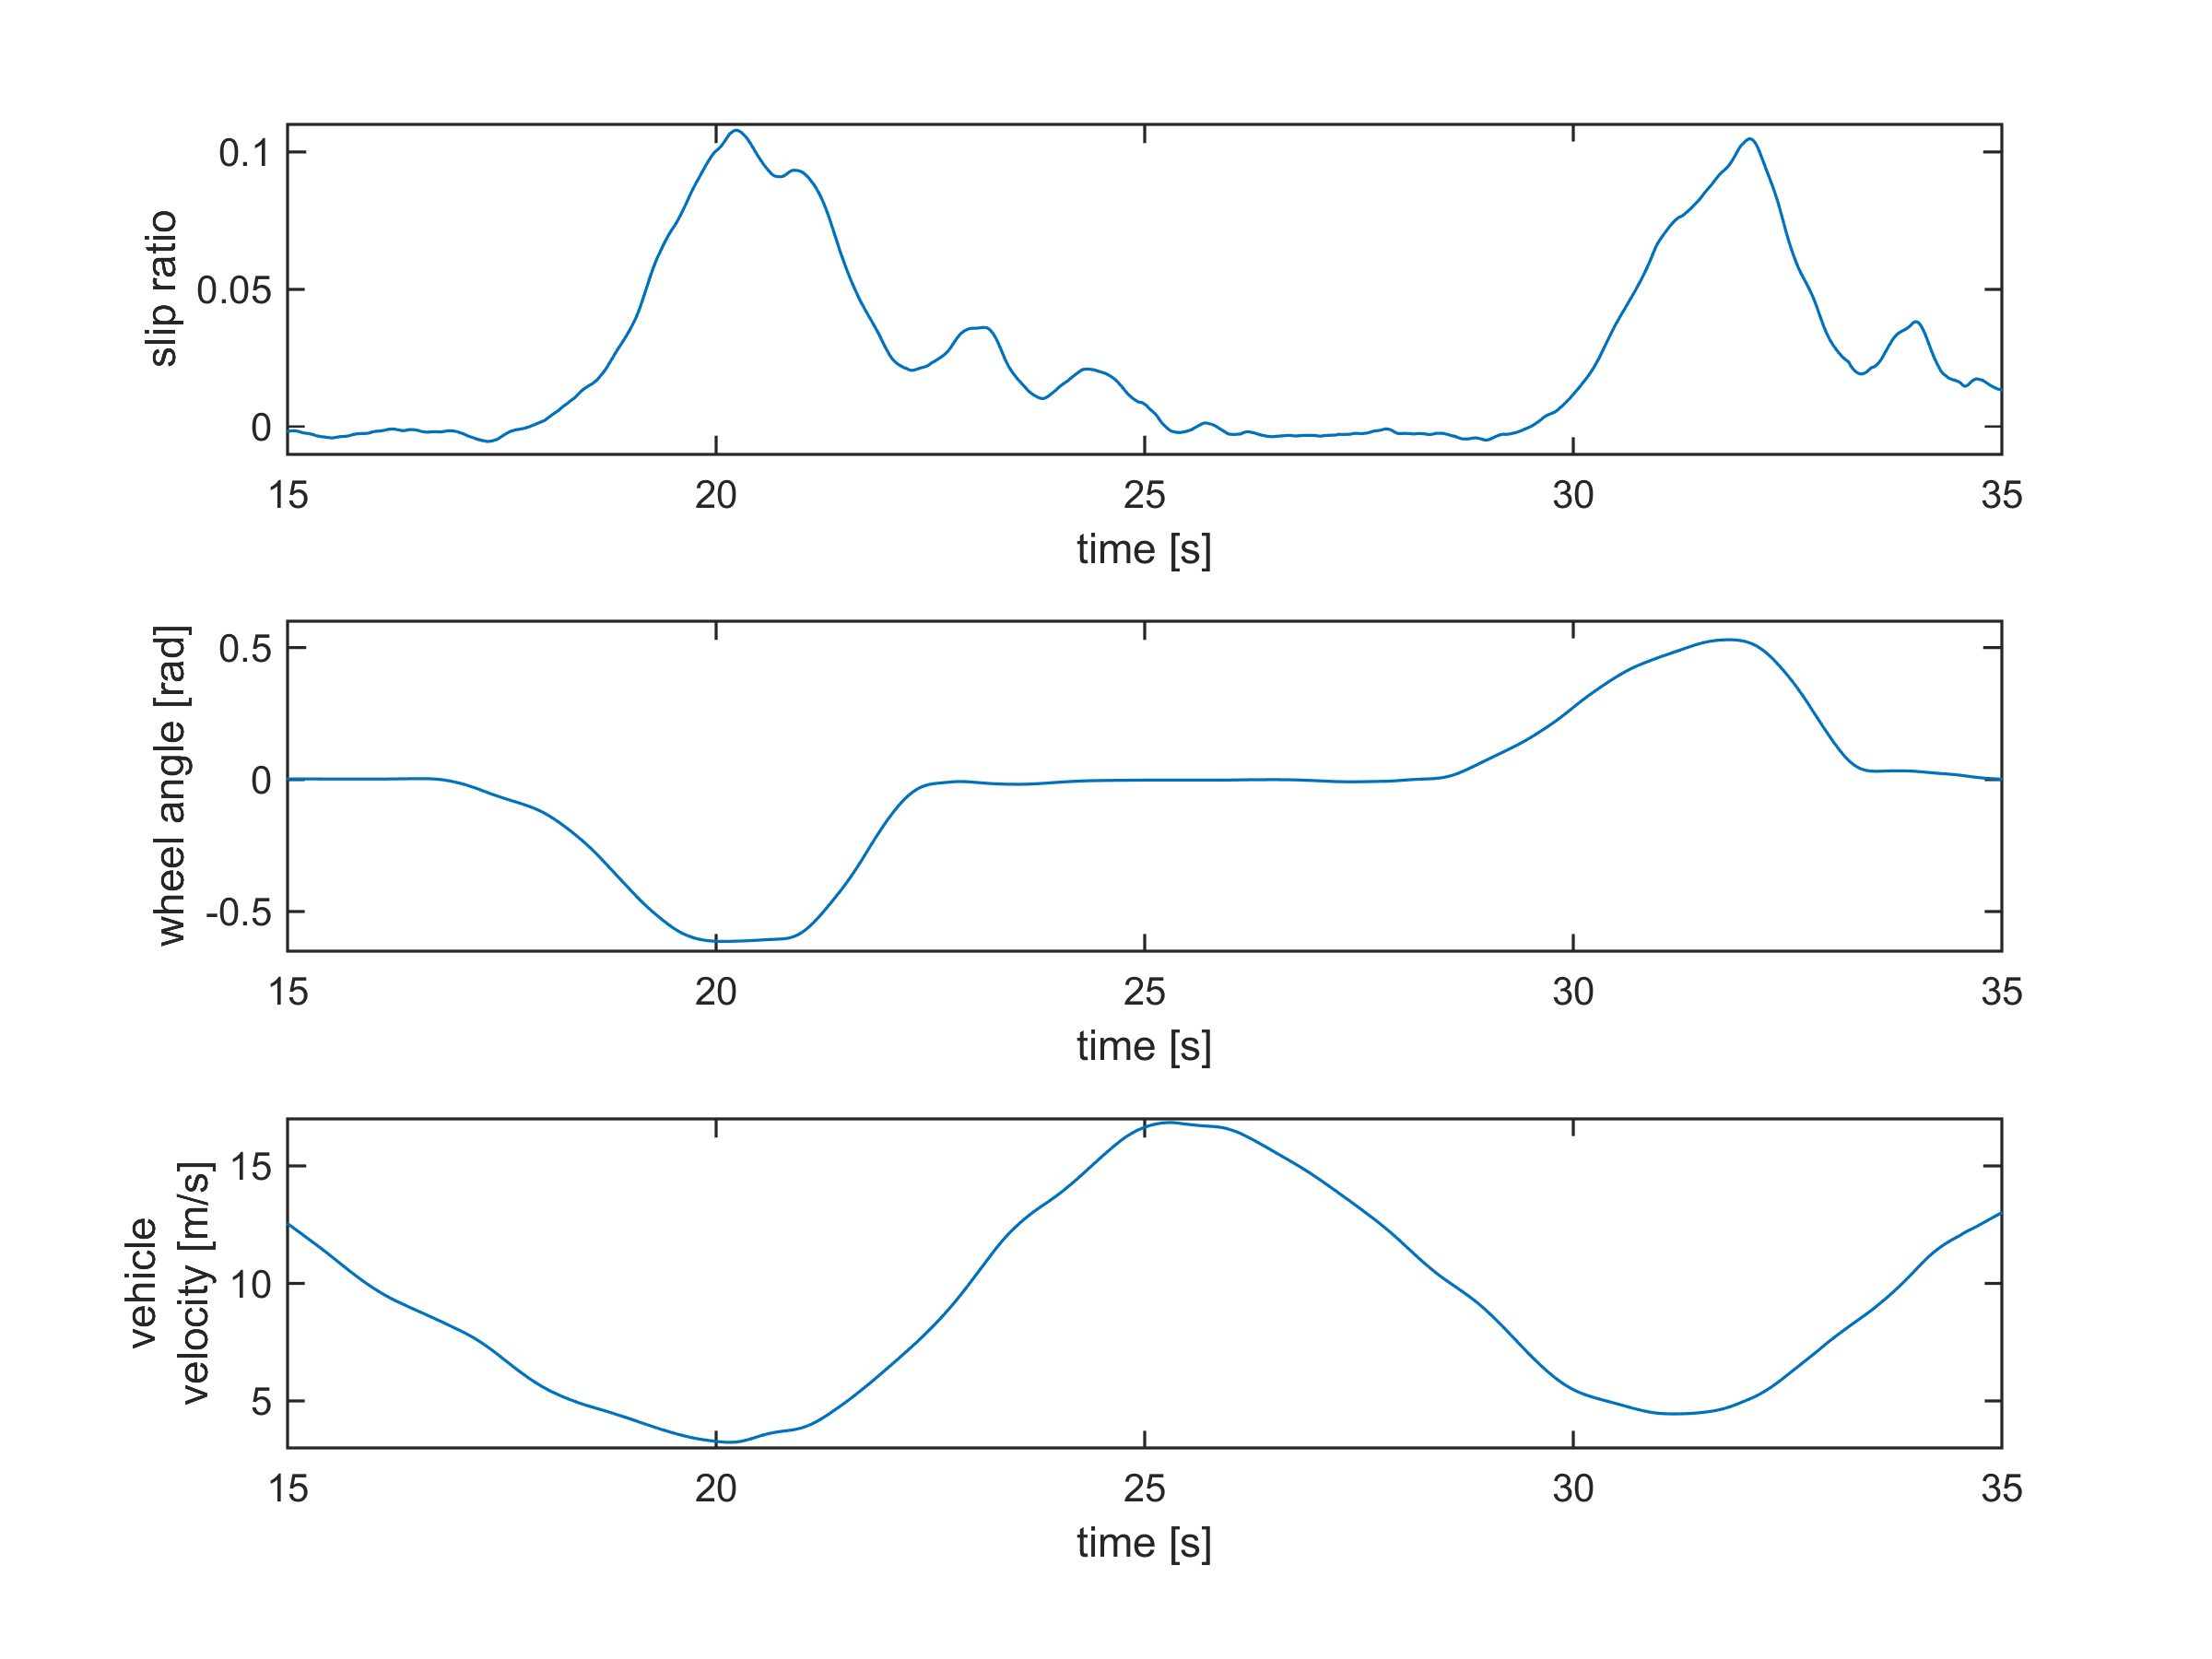
\includegraphics[width=1.0\textwidth]{Pictures/turning_slow_Vx}
	\caption {Large slip values are seen when cornering at a low velocity.}
	\label{turning_slow_Vx}
\end{figure}

Another driving scenario that creates a misleading slip ratio is during acceleration from standing still, which can be seen in figure \ref{slipratio_from_still}, at around $ 2 $ s and $ 24 $ s. When the accelerate begins, the front wheels will start to turn slightly ahead compared to the rear wheels. The percentage difference between the two wheels will become large due to the low velocity, leading to an unreasonable high slip ratio. The same phenomena can also be seen in figure \ref{slipratio_from_still} right before the vehicle comes to a stop, at around $ 22 $ s. 

\begin{figure}[h]
	\centering
	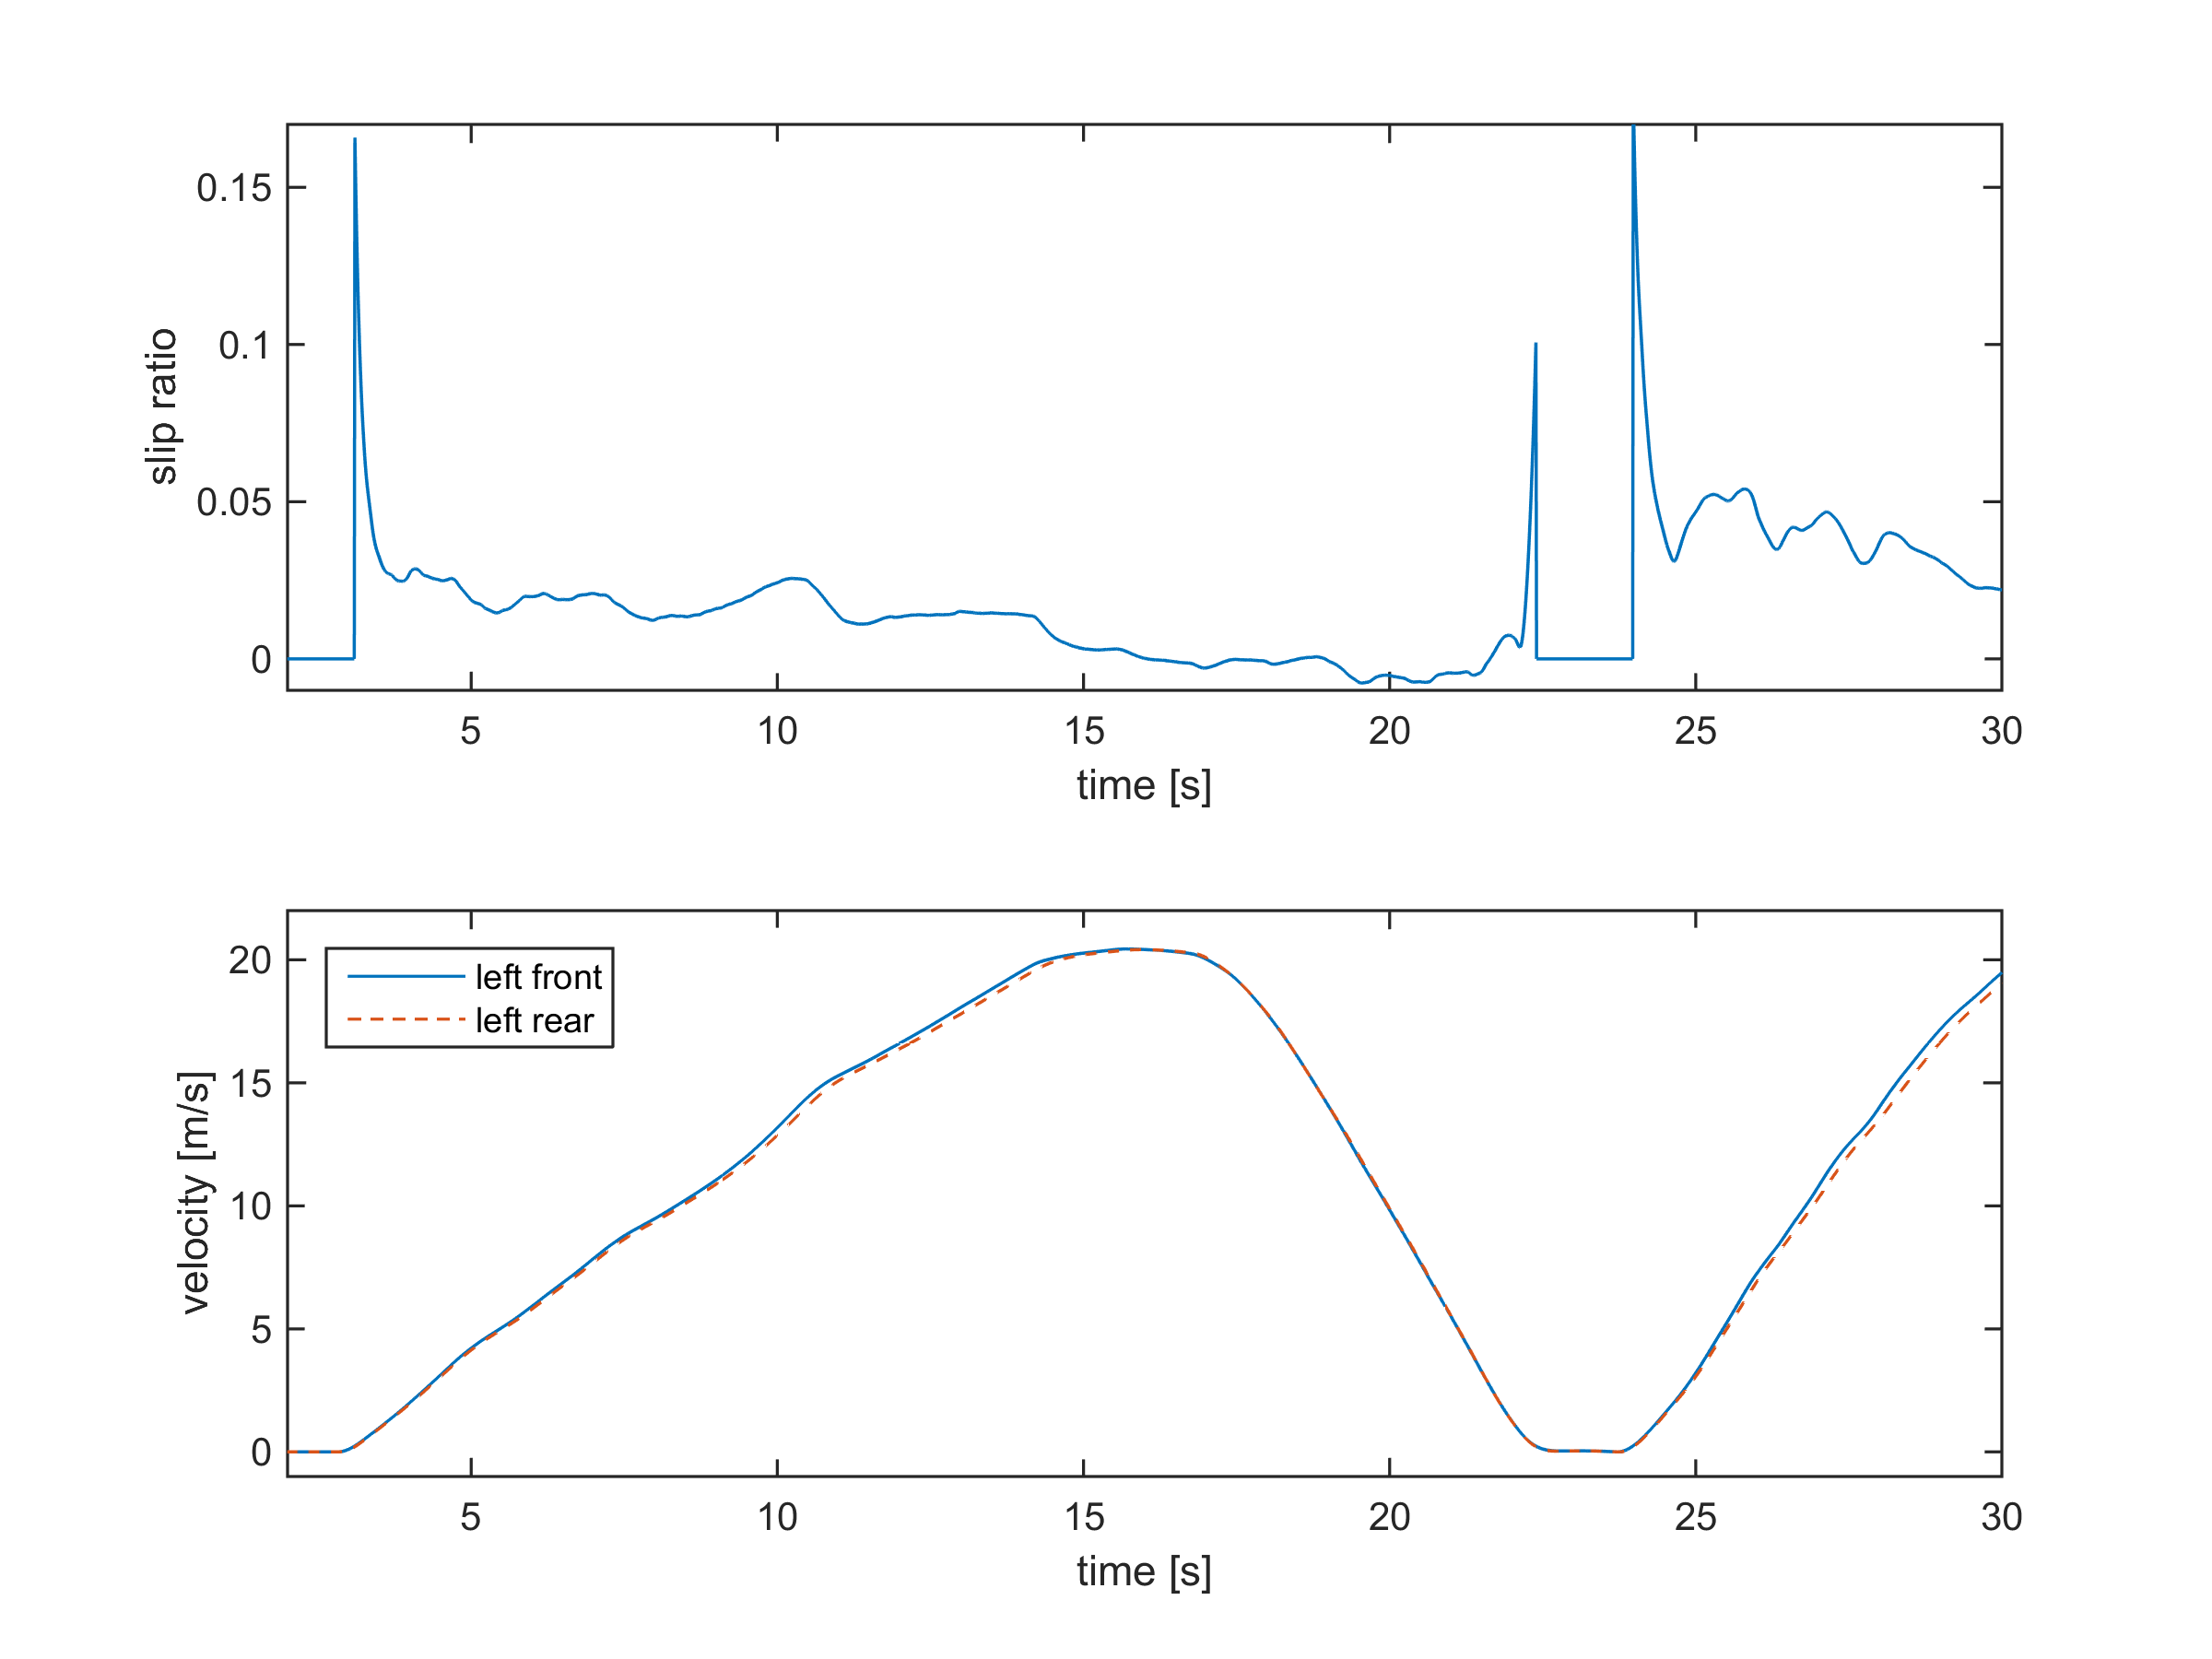
\includegraphics[width=1.0\textwidth]{Pictures/slipratio_from_still}
	\caption {Large slip values are seen when a vehicle begins an acceleration from standing still.}
	\label{slipratio_from_still}
\end{figure}

Limitations has to be set so that the RLS fitting method does not update the estimated friction coefficient at these presented scenarios when the calculated slip ratio gives an unreliable result.

\subsubsection{Limitations due to gear changes}
\label{sec:gearchange}
When a vehicle engages the clutch prior to a gear change, there will be no torque transfered from the engine out to the wheels. Due to filtering and differences between various signals, the force losses in the different models will be different. This can be seen in figure \ref{gear_change}, where gear changes appear at around $ 54.5 $ s and $ 57 $ s.

\begin{figure}[h]
	\centering
	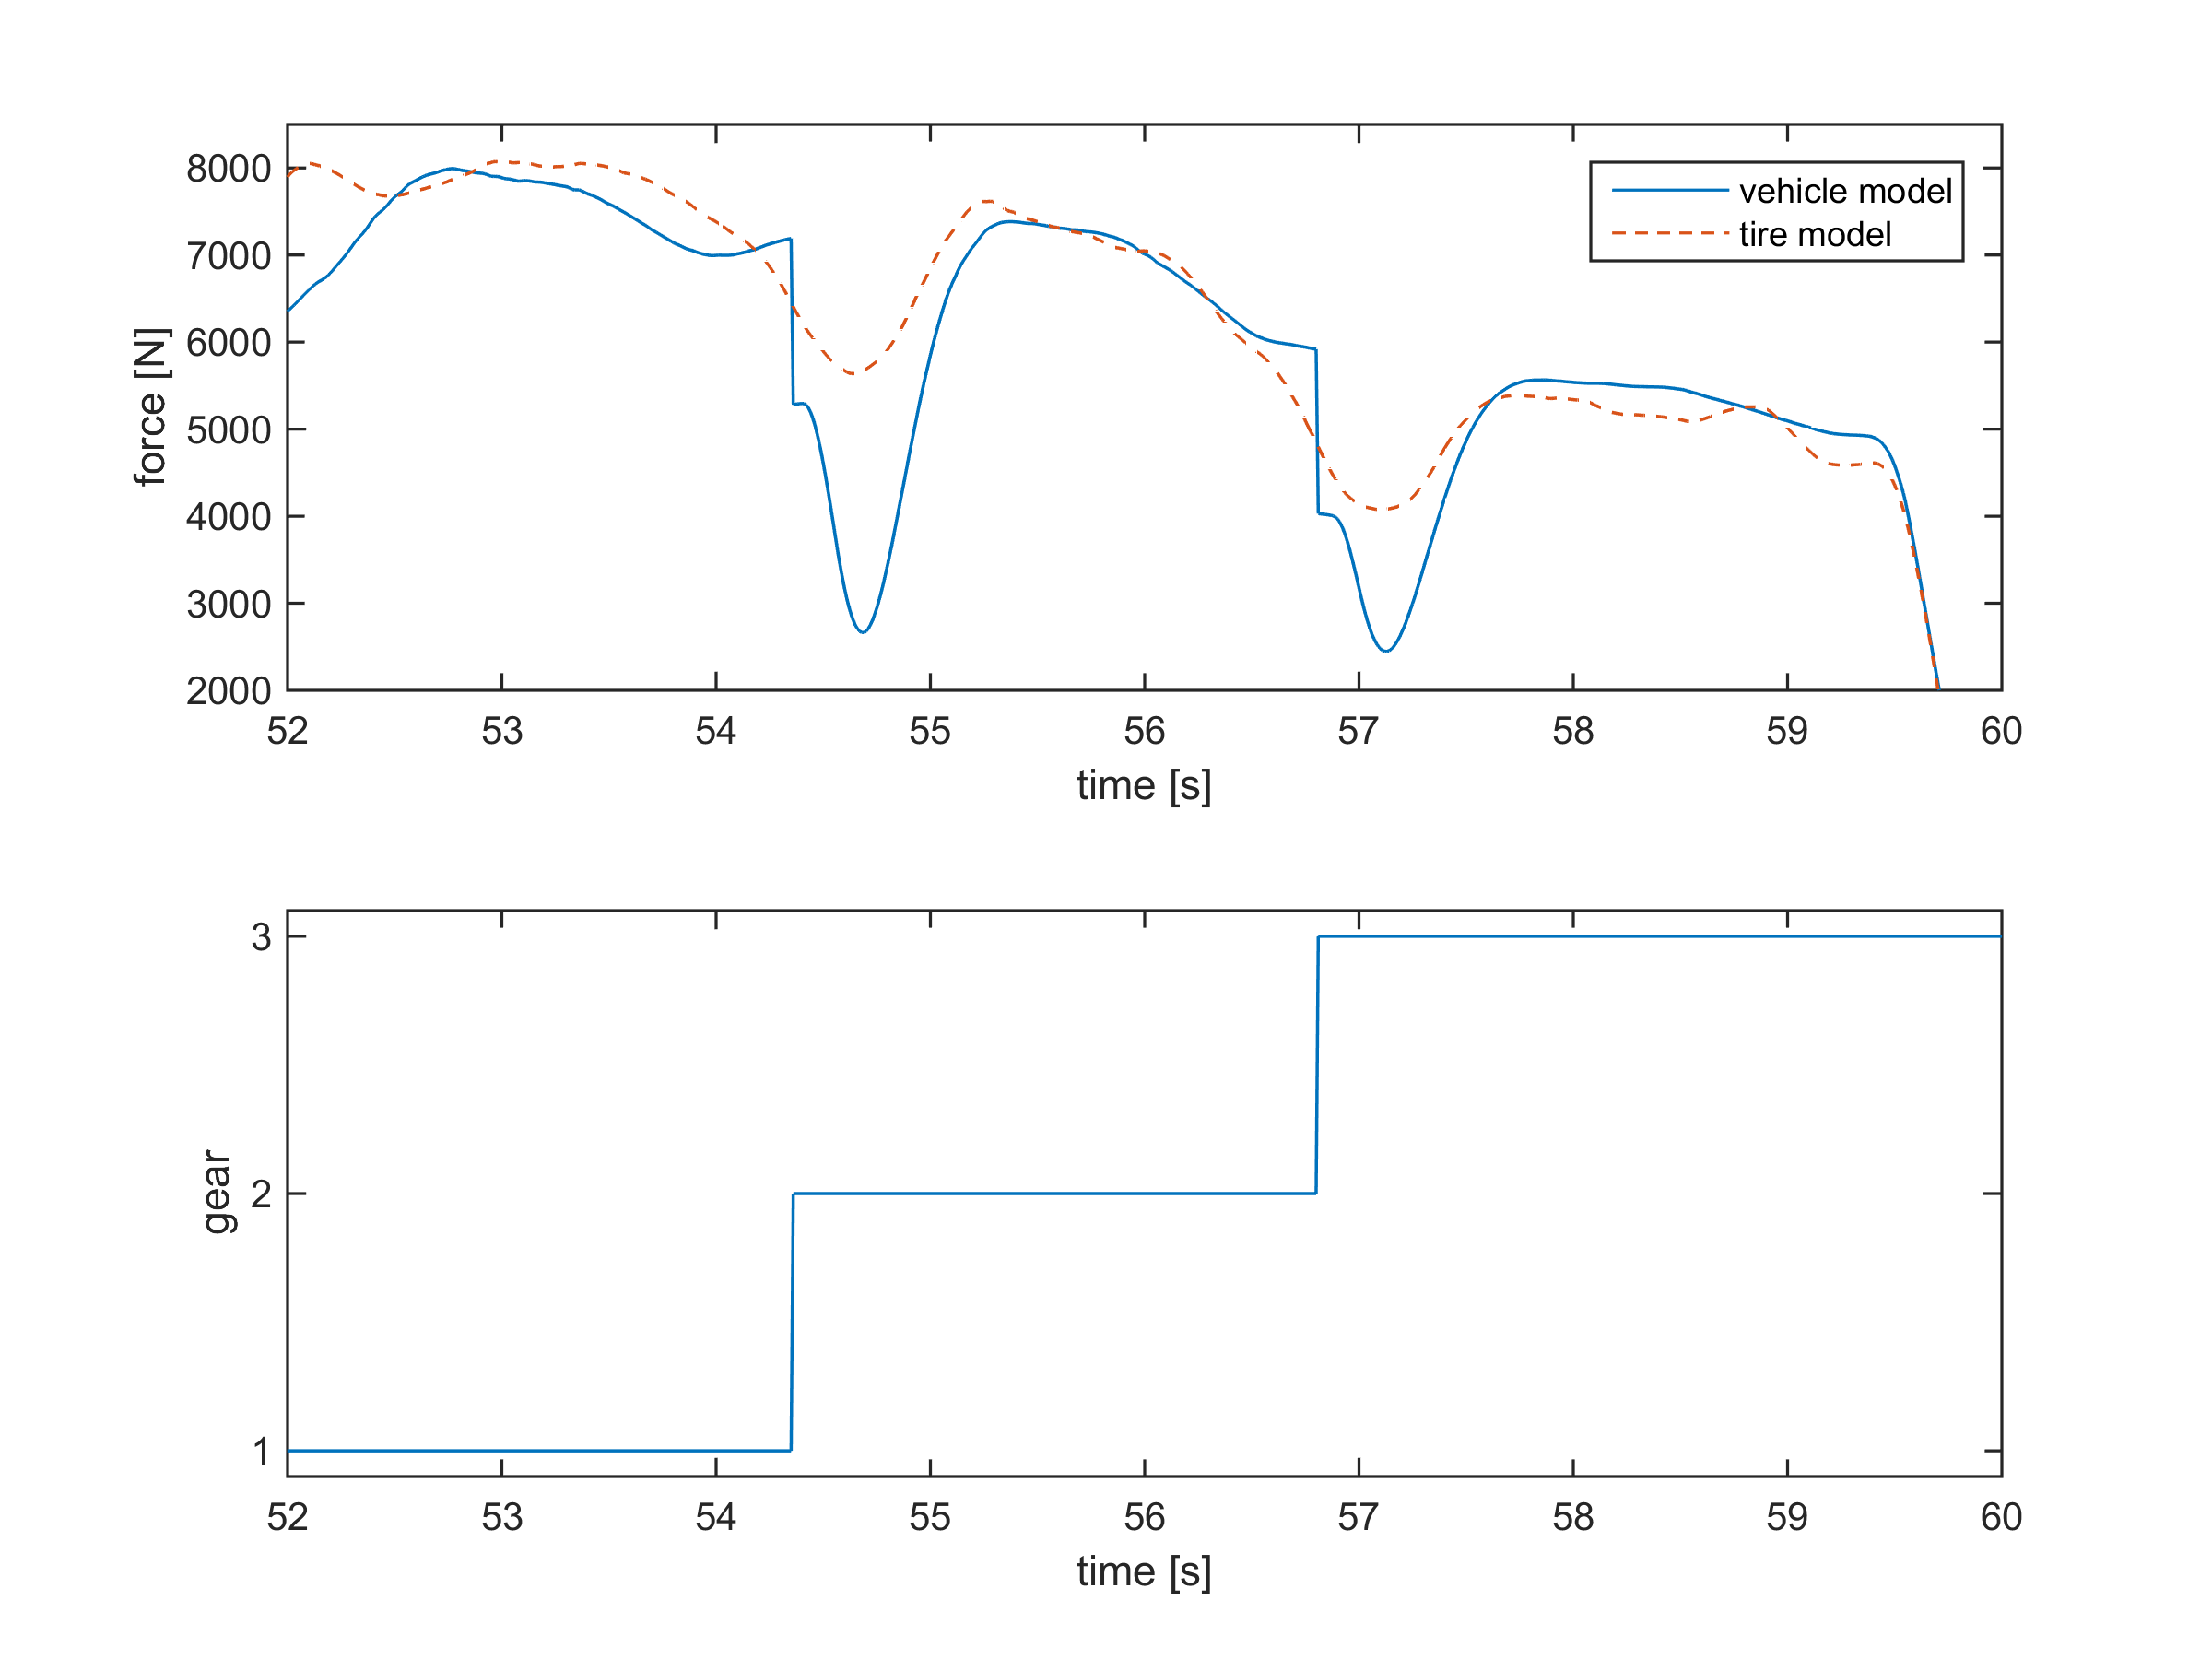
\includegraphics[width=1.0\textwidth]{Pictures/gear_change}
	\caption {Vehicle and tire forces when changing gear.}
	\label{gear_change}
\end{figure}

Due to this disturbance during the gear change, the RLS fitting method should not be updated during a certain amount of time after a gear change occurs. A new friction coefficient can therefore not be calculated during this period. 

\subsubsection{Limitations due to low forces}
Another limitation that adds to the restrictions when the friction coefficient shouldn't be updated is when the total forces acting on the vehicle is too low. During this period of time, when the normalized force is far from the friction coefficient limit, it is very hard to approximate the actual value of the friction coefficient. The reason to this is that the force from the tire model changes less when low forces acting. This can also be seen in figure \ref{different_mue} in section \ref{section_friction coefficient}. It can be seen that amount of force generated for a certain friction coefficient varies very little for the lower slip ratio values. Small errors between the forces from the models will therefore generate a larger change of the friction coefficient which is undesired. 

The RLS should, due to the reasoning above, not be updated when the normalized forces from both the vehicle and tire model is a certain amount below the friction coefficient. This means that the friction coefficient will be updated rarely during calmer driving sequences, which becomes a trade-off to getting a more stable friction coefficient estimator. 

\section{Other methods}

\subsection{Slip-slope friction model}

One friction model that is frequently used and referred to in research papers is the so called slip-slope friction model. The models general idea is that the maximum tire/road friction available can be decided due to its dependency on the slope from the slip-force curve in the linear region. This slip-force curve has the same characteristics as the slip-friction coefficient curve seen in Figure \ref{fric_slip}. 
\begin{equation}
\dfrac{F_{x}}{F_{z}} = k \cdot \kappa
\end{equation}
Where $ F_{x} $ and $ F_{z} $ is the estimated longitudinal and normal force acting on a tire depending on input values. The slip-slope can be estimated with for example recursive least square fitting.
